% --------------------------------------------------------------------------------
%                     __   __        _      _    _
%                     \ \ / /_ _ _ _(_)__ _| |__| |___ ___
%                      \ V / _` | '_| / _` | '_ \ / -_|_-<
%                       \_/\__,_|_| |_\__,_|_.__/_\___/__/
%
% --------------------------------------------------------------------------------
\newcommand{\classname}{extbook}
\newcommand{\innermargin}{3.9cm}
\newcommand{\outermargin}{5.3cm}
\newcommand{\bodyfont}{Equity A}
\newcommand{\headingfont}{Heliotrope 6 Caps}
\newcommand{\sansfont}{Heliotrope 3}
\newcommand{\scfont}{Equity A Caps}
\newcommand{\monospacefont}{Triplicate A}
\newcommand{\Footheadfont}{Heliotrope 4 Caps}
\newcommand{\footheadfont}{Heliotrope 4}
\newcommand{\titlepagename}{compl-titlepage}
\newcommand{\spacingvalue}{1.30}
\newcommand{\headsepvalue}{30pt}
\newcommand{\footskipvalue}{40pt}
\newcommand{\marginparsepvalue}{20pt}
\newcommand{\marginparwidthvalue}{90pt}


% --------------------------------------------------------------------------------
%                          _  _             _
%                         | || |___ __ _ __| |___ _ _
%                         | __ / -_) _` / _` / -_) '_|
%                         |_||_\___\__,_\__,_\___|_|
%
% --------------------------------------------------------------------------------
\documentclass[10pt]{\classname}
\usepackage[T1]{fontenc}
\usepackage[utf8]{inputenc}
\usepackage[italian]{babel}
%\usepackage[document]{ragged2e}
\usepackage{fontspec}
\usepackage{amsmath,amssymb,amsfonts}
\usepackage{amsthm}
\usepackage{mlmodern}
\usepackage[all]{nowidow}
\usepackage{graphicx}
\usepackage{svg}
\usepackage[pdfa]{hyperref}
\usepackage{color}
\usepackage{makecell}
\usepackage{setspace}
\usepackage{parskip}
\usepackage[a4paper, inner=3.8cm, outer=5.4cm]{geometry}
\usepackage{listings}
\definecolor{dkgreen}{rgb}{0.1,0.5,0.1}
\definecolor{greengray}{rgb}{0.517,0.761,0.404}
\definecolor{orange}{rgb}{0.717,0.274,0.105}
\definecolor{blue}{rgb}{0.164,0.317,0.600}
\definecolor{background}{rgb}{0.990,0.990,0.990}
\lstset {
	frame=lrtb,
	language=java,
	aboveskip=0.7cm,
	belowskip=0.2cm,
	showstringspaces=false,
	columns=flexible,
	basicstyle={\small\ttfamily},
	numbers=none,
	backgroundcolor=\color{background},
	numberstyle=\tiny\color{dkgreen},
	keywordstyle=\color{blue},
	commentstyle=\color{greengray},
	stringstyle=\color{orange},
	breaklines=true,
	breakatwhitespace=true,
	tabsize=3
}

\font \bodyfontfs = "\bodyfont"
\font \sansfontfs = "\sansfont"
\font \scfontfs = "\scfont"
\font \monofontfs = "\monospacefont"
\font \Footheadfontfs = "\Footheadfont"
\font \footheadfontfs = "\footheadfont"

\usepackage{fancyhdr}
\pagestyle{fancy}
\fancyhf{}
\fancyhead[LE,RO]{\Footheadfontfs \nouppercase \leftmark}
\fancyfoot[CE,CO]{\footheadfontfs \thepage}
\renewcommand{\headrulewidth}{1.0pt}
\renewcommand{\footrulewidth}{1.0pt}
\renewcommand{\chaptermark}[1]{\markboth{#1}{}}

%\theoremstyle{theorem}
\newtheorem{thm}{Teorema}
\setlength{\tabcolsep}{0.5em} % for the horizontal padding
{\renewcommand{\arraystretch}{1.35}% for the vertical padding

\theoremstyle{definition}
\newtheorem{definizione}{Definizione}[section]
\setlength{\tabcolsep}{0.5em} % for the horizontal padding
{\renewcommand{\arraystretch}{1.35}% for the vertical padding


\theoremstyle{definition}
\newtheorem{identita}{Identità}[section]
\setlength{\tabcolsep}{0.5em} % for the horizontal padding
{\renewcommand{\arraystretch}{1.35}% for the vertical padding

\begin{document}
\setmainfont{\bodyfont}
\setsansfont{\sansfont}
\setmonofont{\monospacefont}

\include{\titlepagename}
%\title{Title}
%\author{Author}
%\maketitle

\setstretch{\spacingvalue}
\setlength{\emergencystretch}{0pt}
\pretolerance=150
\tolerance=250
\hbadness=150
\hfuzz=0pt
\setlength{\headsep}{\headsepvalue}
\setlength{\footskip}{\footskipvalue}
\setlength{\marginparsep}{\marginparsepvalue}
\setlength{\marginparwidth}{\marginparwidthvalue}

\tableofcontents

\let\oldtextsc\textsc
\renewcommand{\textsc}[1]{\oldtextsc{\scfontfs #1}}
\let\oldpart\part
\renewcommand{\part}[1]{\setmainfont{\headingfont}\oldpart{#1}\setmainfont{\bodyfont}}
\let\oldchapter\chapter
\renewcommand{\chapter}[1]{\setmainfont{\headingfont}\oldchapter{#1}\setmainfont{\bodyfont}}
\let\oldsection\section
\renewcommand{\section}[1]{\setmainfont{\headingfont}\oldsection{#1}\setmainfont{\bodyfont}}
\let\oldsubsection\subsection
\renewcommand{\subsection}[1]{\setmainfont{\headingfont}\oldsubsection{#1}\setmainfont{\bodyfont}}
\let\oldsubsubsection\subsubsection
\renewcommand{\subsubsection}[1]{\setmainfont{\headingfont}\oldsubsubsection{#1}\setmainfont{\bodyfont}}


% --------------------------------------------------------------------------------
%                     ___                             _
%                    |   \ ___  __ _  _ _ __  ___ _ _| |_
%                    | |) / _ \/ _| || | '  \/ -_) ' \  _|
%                    |___/\___/\__|\_,_|_|_|_\___|_||_\__|
%
% --------------------------------------------------------------------------------


\chapter{La macchina di Turing}
\section{Descrizione della macchina}

Una \textbf{macchina di Turing} è una \textsc{macchina} che è descritta da un insieme di
\emph{simboli} $\Gamma = \{\alpha, \beta, \gamma, \delta, \dots\}$ \emph{finito} e da
un insieme di \emph{stati} $\mathcal{Q} = \{q_1, q_2, \dots, q_n\}$ anch'esso
\emph{finito}. La macchina di Turing dispone di un nastro di memoria
\emph{potenzialmente illimitato} a destra e a sinistra, avente delle celle
contenenti i simboli; essa identifica il simbolo nella posizione dove la
\emph{testina} della macchina è collocata sul nastro. Ad ogni iterazione della
macchina di Turing viene letto il simbolo, e a seconda dello stato $q_i$, viene
intrapresa un'azione fra le $3$ seguenti:
\begin{itemize}
    \item spostamento della testina a destra;
    \item spostamento della testina a sinistra;
    \item riscrittura del simbolo sotto la testina con uno qualsiasi
        appartenente all'alfabeto di simboli.
\end{itemize}

Nello specifico, una macchina di Turing è univocamente identificata dalla sua
\emph{matrice di transizione} $\delta  : \mathcal Q \times \Gamma \rightarrow
\mathcal Q \times (\Gamma \cup \{L,R\})$\footnote{In talune circostanze, è
possibile trovare una definizione differente, cioè $$\delta  : \mathcal Q \times
\Gamma \rightarrow \mathcal Q \times \Gamma \times \{L,R\};$$ in altre parole, è
una macchina che \emph{si muove sempre sul nastro,} poiché per ogni stato è
sempre definito un movimento. Per questo tipo di macchina, sono necessarie
diverse regole d'ingaggio, e i programmi in essa costruiti saranno radicalmente
differenti. La differenza fra i due modelli rappresenta un'evidenza della
versatilità della macchina di Turing, e della possibilità di introdurla con
varie definizioni, dove ciascuna delle quali possiede le proprie peculiarità.},
dove i simboli $L$ ed $R$ sono rappresentativi dell'azione di spostarsi,
rispettivamente, a sinistra e a destra del nastro di memoria. La matrice di
transizione lega, dunque, ciascuno stato al simbolo collocato immediatamente
sotto alla testina nel nastro di memoria, stabilendo in maniera univoca
l'azione da intraprendere. Si può dire dunque che la matrice di transizione
fornisce alla macchina di Turing l'elenco delle possibili azioni da
intraprendere, alla lettura di un simbolo sulla cella corrente, a seconda dello
stato in cui si trova. L'insieme delle azioni che la macchina di Turing compie
è quindi la realizzazione del programma stesso, quello che nei termini del
modello RAM si sarebbe detto essere la sequenza di istruzioni elementari. In
parole povere, non si scrive un vero e proprio programma come nel caso della
macchina a modello RAM, bensì si specifica il passo da compiere alla lettura di
un determinato simbolo sul nastro. I passi sono riportati in questa tabella, la
matrice di transizione, e lì si descrive il meccanismo della macchina.

Una macchina di Turing può anche essere accompagnata da un alfabeto
\emph{ausiliario}, ovverosia da un alfabeto $\mathcal V$ comprendente simboli
simili a quelli di $\Gamma$, ma che vengono utilizzati qualora la macchina di
Turing avesse \emph{già processato} la cella in questione (i simboli ausiliari
sono ``simili'' a quelli dell'alfabeto tradizionale, ma hanno una differenza
che ne permette la distinzione). Tipicamente, l'utilizzo dell'alfabeto
ausiliario è importante nel caso specifico in cui si adoperino procedure per le
quali è utile ricordare se una cella sia già stata in precedenza processata
dalla macchina di Turing, oppure no --- in ogni caso, l'alfabeto ausiliario è
meramente un sussidio che permette una semplificazione della procedura o aiuta
ad interpretare il comportamento della macchina, non è in nessun modo un
qualsivoglia tipo di estensione della macchina di Turing. Come sarà mostrato in
seguito, ciascuna altra possibile definizione di macchina di Turing è, dal
punto di vista della potenza computazione, del tutto equivalente alla
definizione già data sopra. In parole povere, ci facciamo aiutare dall'alfabeto
ausiliario per ``ricordarci'' su quali celle siamo già passati.


\begin{table}[ht]
\centering
\begin{tabular}{c|cccc}
    & $q_1$ & $q_2$ & $\cdots$ & $q_n$ \\
    \hline
$\alpha$ & $\beta/q_2$ & $\gamma/q_2$ & $\cdots$ & \\
$\beta$ & $L/q_1$ & $\gamma/q_3$ & $\cdots$ & \\
$\gamma$ & $\gamma/q_3$ & $R/q_2$ & $\cdots$ & \\
$\vdots$ & $\vdots$ & $\vdots$ & $\ddots$ &    
\end{tabular}
\caption{Possibile matrice di transizione per una macchina di Turing. Le righe
corrispondono ai simboli dell'alfabeto $\Gamma$, mentre le colonne sono
corrispondenti ai singoli stati dell'insieme $\mathcal
Q$. Ogni elemento della tabella indica il simbolo da scrivere/stato in cui la
macchina dovrà trovarsi al passo successivo,}\label{tab:matriceTransizione}
\end{table}
\bigskip


Diversamente dal modello RAM, la quantità di memoria destinata ad ogni cella è
\emph{limitata}, poiché vi può essere collocato soltanto un numero finito di
simboli, quelli appunto dell'insieme $\Gamma$. Qua non si possono più inserire
numeri grandissimi, bensì bisogna accontentarsi dei simboli che abbiamo inserito
nel nostro alfabeto, un numero finito di essi. Ciononostante, la macchina di
Turing ha dei vantaggi, ad esempio si presta meglio alla trattazione di
stringhe, poiché i simboli possono rappresentare qualsivoglia tipologia di
entità astratta, mentre per il modello RAM si avrebbe necessità di una codifica
fra numeri reali e simboli da trattare. Non vi è più dunque la limitazione
imposta dal fatto che all'interno di una cella possa risiedere esclusivamente
un numero naturale, non importa quanto grande sia; nella macchina di Turing le
celle possono contenere simboli di qualsiasi natura essi siano. Lo
``svantaggio'', tuttavia, è che all'interno di ogni cella non può essere
contenuta una quantità \emph{arbitraria} di informazione, come invece avveniva
per il modello RAM, che faceva uso dei numeri naturali. In ogni caso, le due
macchine sono equivalenti, quindi possiamo in qualche modo ``scavalcare''
questa limitazione che solo in apparenza è limitante.

Tipicamente, assieme all'alfabeto che definisce una macchina di Turing viene definito
un sottoinsieme sigma di \emph{simboli di input}, $\Sigma \subset \Gamma$, in
concomitanza al quale viene definito un simbolo vuoto, \emph{blank}, $b \in
\Gamma - \Sigma$. Il simbolo $b$ incarna dunque l'idea di \emph{cella
vuota} --- si pensi infatti al valore che una cella di memoria primaria
qualsiasi di un computer reale avrebbe, al momento immediatamente successivo
all'accensione: essa risulterebbe posta allo zero logico, di fatto non
conterrebbe alcun valore d'interesse, dato che essa non è ancora stata
``toccata'' dall'esecuzione di alcun programma. Il simbolo \emph{blank} sta a
significare proprio questo, ed è l'equivalente del valore `zero' del modello
RAM, dove all'avvio del programma ogni cella di memoria fuorché quelle
contenenti i valori di ingresso contiene il numero reale $0$. 

Ricapitolando, ogni macchina di Turing viene univocamente definita da:
\begin{itemize}
    \item un insieme finito di simboli $\Gamma$ --- essi comprendono sia i
        simboli di input $\Sigma$ che il simbolo \emph{blank} $b$;
    \item un insieme finito di stati $\mathcal Q$;
    \item una funzione (matrice) di transizione $\delta  : \mathcal Q \times
        \Gamma \rightarrow \mathcal Q \times (\Gamma \cup \{L,R\})$.
\end{itemize}

Una diversa maniera per definire una macchina di Turing è tramite la
\emph{quaterna} o \emph{quadrupla} $q_i, s_j, \alpha, q_k$, dove $q_i$ è lo
\emph{stato in cui si trova la macchina}, $s_j$ è il \emph{simbolo letto dalla
testina}, $\alpha$ è il \emph{simbolo scritto nella matrice di transizione} e
$q_k$ è lo \emph{stato successivo} in cui la macchina di Turing si troverà al
termine dell'esecuzione di $\alpha$. In particolare, l'operazione che la
macchina di Turing effettua dipende dal simbolo $\alpha$ scritto nella matrice
di transizione:
\begin{itemize}
    \item se $\alpha = s_i$, sostituisci il simbolo $s_j$ con $s_i$;
    \item se $\alpha = R$, muovi la testina a destra;
    \item se $\alpha = L$, muovi la testina a sinistra.
\end{itemize}

L'insieme di tutte queste quaterne descrive l'insieme dei possibili
comportamenti della macchina di Turing, dunque questo elenco è del tutto
equivalente ad una matrice di transizione per come la abbiamo definita in
precedenza.

In parole povere, anche così definita una macchina di Turing può sovrascrivere
un simbolo presente sulla cella con un altro presente nel suo alfabeto,
$\Gamma$, può spostare la testina di un'unità a destra, e può fare altrettanto
a sinistra.

Resta da scogliere il nodo relativo alla terminazione della macchina di Turing.
Nel modello RAM, la terminazione avveniva qualora le istruzioni si fossero
esaurite, o più precisamente qualora l'indice dell'istruzione successiva fosse
quello di un'istruzione assente nella sequenza che definisce la procedura. In
assenza del concetto di ``istruzione'', secondo quale regole dovrebbe terminare
una macchina di Turing? 

Lo \emph{stop} della computazione di una macchina di Turing avviene qualora la
coppia $q_i, s_j$ \textbf{non} sia presente nella matrice di transizione. Nel
caso di una coppia simbolo---stato non presente nella matrice di transizione,
la macchina di Turing avrà terminazione, e vi sarà il riconoscimento del valore
finale di computazione, espresso similmente al caso del modello RAM con una
convenzione che permetta di identificare il valore finale del risultato della
computazione. Dunque, una macchina di Turing si ferma quando non sa più che fare.

Se lo stop della computazione è stato chiarito, ora resta da definire il metodo
con cui andremo a recuperare il valore finale della computazione. Se per una
macchina modello RAM potevamo recuperare il valore alla cella 0, con una
macchina di Turing ciò non è più possibile (come possiamo, infatti,
immagazzinare in una singola cella un numero arbitrariamente grande? È evidente
che con questa limitazione già citata nei paragrafi precedenti dobbiamo
escogitare un nuovo stratagemma per ovviare al problema).
Convenzionalmente, l'esito di una macchina di Turing è una particolare
configurazione di memoria dello stato finale. Si è infatti scelto che
il risultato $f(x)$ sia da leggersi come il numero totale di occorrenze di simboli $1$
(meno un'occorrenza) sul nastro nella configurazione iniziale, se la computazione è
andata a convergenza, mentre il risultato sarà da considerarsi indefinito
altrimenti. La sequenza di occorrenze del simbolo $1$ verrà delimitata dal
carattere \emph{blank}. Quindi vi saranno $f(x) + 1$ simboli
\textquotesingle1\textquotesingle, e pertanto sarà da contare un simbolo
\textquotesingle1\textquotesingle\ in meno (lo
\textquotesingle0\textquotesingle\   sarà indicato con la presenza di un
singolo simbolo \textquotesingle1\textquotesingle, per il risultato
\textquotesingle1\textquotesingle\ saranno necessari invece 2 simboli
\textquotesingle1\textquotesingle di fila, e così via). Per quanto invece
riguarda i risultati di tipo \emph{vettoriale}, cioè del tipo
$f(x_1,x_2,\dots,x_n)$, ebbene sarà sufficiente costruire $n$ ``quadrati'' in
cui racchiudere gli $x+1$ simboli $1$, ciascuno delimitato dal simbolo
\emph{b}. In altre parole, la situazione è quella descritta dalla
Figura~\ref{fig:mdtRisultato}.

Per farla breve, preleveremo il risultato $x$ secondo la formula $$x = \# \mbox{ di simboli } 1 \mbox{ delimitato da due caratteri blank, sottratto uno}.$$

\begin{figure}[b]
    \centering
    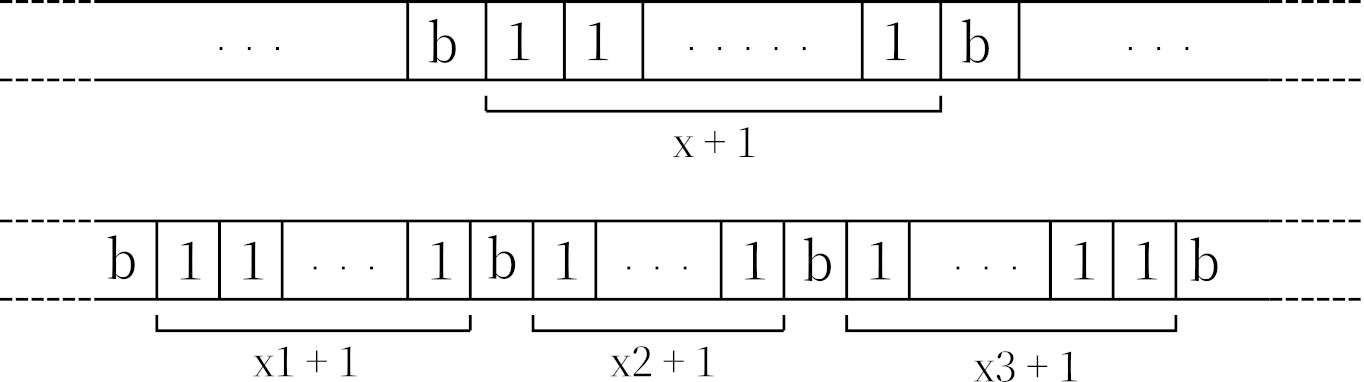
\includegraphics[ width=1.0\linewidth, height=\textheight, keepaspectratio]{./pics/mdtRisultato.jpg}
    \caption{Risultato singolo (sopra) e \emph{vettoriale} (sotto) di una macchina di Turing.}
    \label{fig:mdtRisultato}
\end{figure}



Un difetto evidente della macchina di Turing è la sua difficoltà di trattazione. 
Per via dell'utilizzo tramite la matrice di transizione è particolarmente
difficile scrivere programmi per una macchina di Turing~--~questo è principalmente
dovuto al fatto che la macchina di Turing è una macchina `a stati', dove non vi è
un insieme di istruzioni da applicare direttamente, ma è necessario determinare
prima di tutto la matrice di transizione relativa a ciò che bisogna calcolare,
stato per stato e simbolo per simbolo. Il programma non è più esprimibile come
una successione di passi ``dall'alto verso il basso'', ma va scritto sotto
forma di una criptica matrice di transizione dove i passi da definire sono
quelli compiuti da una macchina di Turing a fronte di un determinato simbolo.

Una macchina di Turing, non importa come sia stata definita, può essere
adoperata sostanzialmente per compiere $3$ operazioni:
\begin{enumerate}
    \item per il \emph{calcolo} di una funzione --- in questo caso la macchina di Turing è
        intesa come \emph{calcolatore}, e lo scopo è quello banalmente di calcolare una
        funzione $f: \mathbb{N}^n \rightarrow \mathbb{N}$. In questo caso, la
        macchina di Turing risulta essere meno efficiente del modello RAM, per
        via dell'assenza del comodo sistema di istruzioni presente in quest
        ultimo. Cionondimeno, essa può compiere ugualmente il calcolo con la medesima capacità;
    \item per il \emph{riconoscimento} di una stringa --- la macchina di
        Turing è intesa come \emph{accettore}. In questo contesto la macchina di Turing è
        di gran lunga più efficiente del modello RAM, poiché non è richiesta la
        codifica da numeri naturali a simboli, necessaria invece se si ha a che fare esclusivamente con numeri naturali;
    \item per la \emph{decisione} di un predicato --- la macchina di Turing è
        intesa come \emph{decisore}.
\end{enumerate}

\subsection{Equivalenza fra macchina di Turing e $\mathcal R$}

Un importante primo teorema definisce l'equivalenza della macchina di Turing (avente
insieme delle funzioni computabili $\mathcal{TC}$ all'insieme delle funzioni
parziali ricorsive $\mathcal R$, e lo lega indissolubilmente all'insieme delle
funzioni computabili dal modello RAM $\mathcal C$.

%\begin{center}\vspace*{0.6cm}\rule{1.0\textwidth}{1.2pt}\vspace*{0.4cm}\end{center}

\begin{thm}[dell'equivalenza della macchina di Turing all'insieme $\mathcal R$ delle funzioni parziali ricorsive]

    Per esso vale che
    $$\mathcal R \equiv \mathcal {TC} \equiv \mathcal C,$$ ovverosia gli
    insiemi delle funzioni Turing--computabili $\mathcal{TC}$, delle funzioni
    parziali ricorsive $\mathcal R$ e delle funzioni computabili dal modello
    RAM $\mathcal C$ sono \emph{equivalenti}.
\end{thm}

\textsc{Dimostrazione} --- Un possibile spunto di dimostrazione di $\mathcal {TC} \subseteq \mathcal R$ si
ha grazie al fatto che la configurazione e lo stato della MdT durante la
computazione possono essere codificati da un numero naturale; le operazioni
sulla macchina sono rappresentate da funzioni ricorsive su questi numeri. Il
viceversa è invece mostrabile tenendo conto che si può verificare che
$\mathcal{TC}$ contiene le funzioni di base ed è chiusa rispetto a sostituzione,
ricorsione e minimazione illimitata.

\begin{flushright}
$\blacksquare$
\end{flushright}

%\begin{center}\vspace*{0.6cm}\rule{1.0\textwidth}{1.2pt}\vspace*{0.4cm}\end{center}


\subsection{Macchina di Turing per il calcolo della somma}

Supponiamo di voler fare la somma fra due numeri interi naturali, $x$ ed $y$.
In questo caso, la macchina di Turing dovrebbe calcolare la funzione $f(x,y) =
x + y$. Per fare ciò, costruiremo gli elementi fondamentali della macchina di
Turing. In particolare, avremo che l'alfabeto di simboli $\Gamma = \{0, 1,
b\}$, cioè avremo bisogno esclusivamente di $2$ simboli eccezion fatta per il
simbolo \emph{blank}, mentre invece faremo uso di $3$ stati $\mathcal Q =
\{q_1, q_2, q_3\}$. Lo stato iniziale è lo stato $q_1$, mentre lo stato finale
è $q_3$. Resta ora da definire la matrice di transizione. Uno fra i tanti modi
di definirla è il seguente (faremo uso delle quadruple),


\begin{table}[ht]
\centering
\begin{tabular}{cccc}
    $q_1$ & $1$ & $b$ & $q_1$\\
    $q_1$ & $b$ & $R$ & $q_2$\\
    $q_2$ & $1$ & $b$ & $q_3$\\
    $q_2$ & $b$ & $R$ & $q_2$

\end{tabular}
\caption{Matrice di transizione per la macchina di Turing che calcola $f(x,y) =
x + y$, espressa a quadruple.}\label{tab:mdtSomma}
\end{table}
\bigskip

L'idea è quella di togliere due simboli $1$, di modo che gli $1$ rimanenti
corrispondano al valore del risultato finale. Infatti, provando a calcolare
$f(2, 1) = 3$ avremo che

\begin{table}[ht]
\centering
\begin{tabular}{cccccccc}
   $q_1$&     &     &     &     &     &     &     \\
    $1$ & $1$ & $1$ & $b$ & $1$ & $1$ & $b$ & $b$ \\
   $q_1$&     &     &     &     &     &     &     \\
    $b$ & $1$ & $1$ & $b$ & $1$ & $1$ & $b$ & $b$ \\
        &$q_2$&     &     &     &     &     &     \\
    $b$ & $1$ & $1$ & $b$ & $1$ & $1$ & $b$ & $b$ \\
        &     &$q_3$&     &     &     &     &     \\
    $b$ & $b$ & $1$ & $b$ & $1$ & $1$ & $b$ & $b$
\end{tabular}
\end{table}
\bigskip

ed il numero finale di simboli $1$ corrisponde proprio al valore della somma,
$2 + 1 = 3$.

Possiamo anche costruire un grafo della macchina di cui sopra, mostrato in
Figura~\ref{fig:mdtSomma}.


\begin{figure}[b]
    \centering
    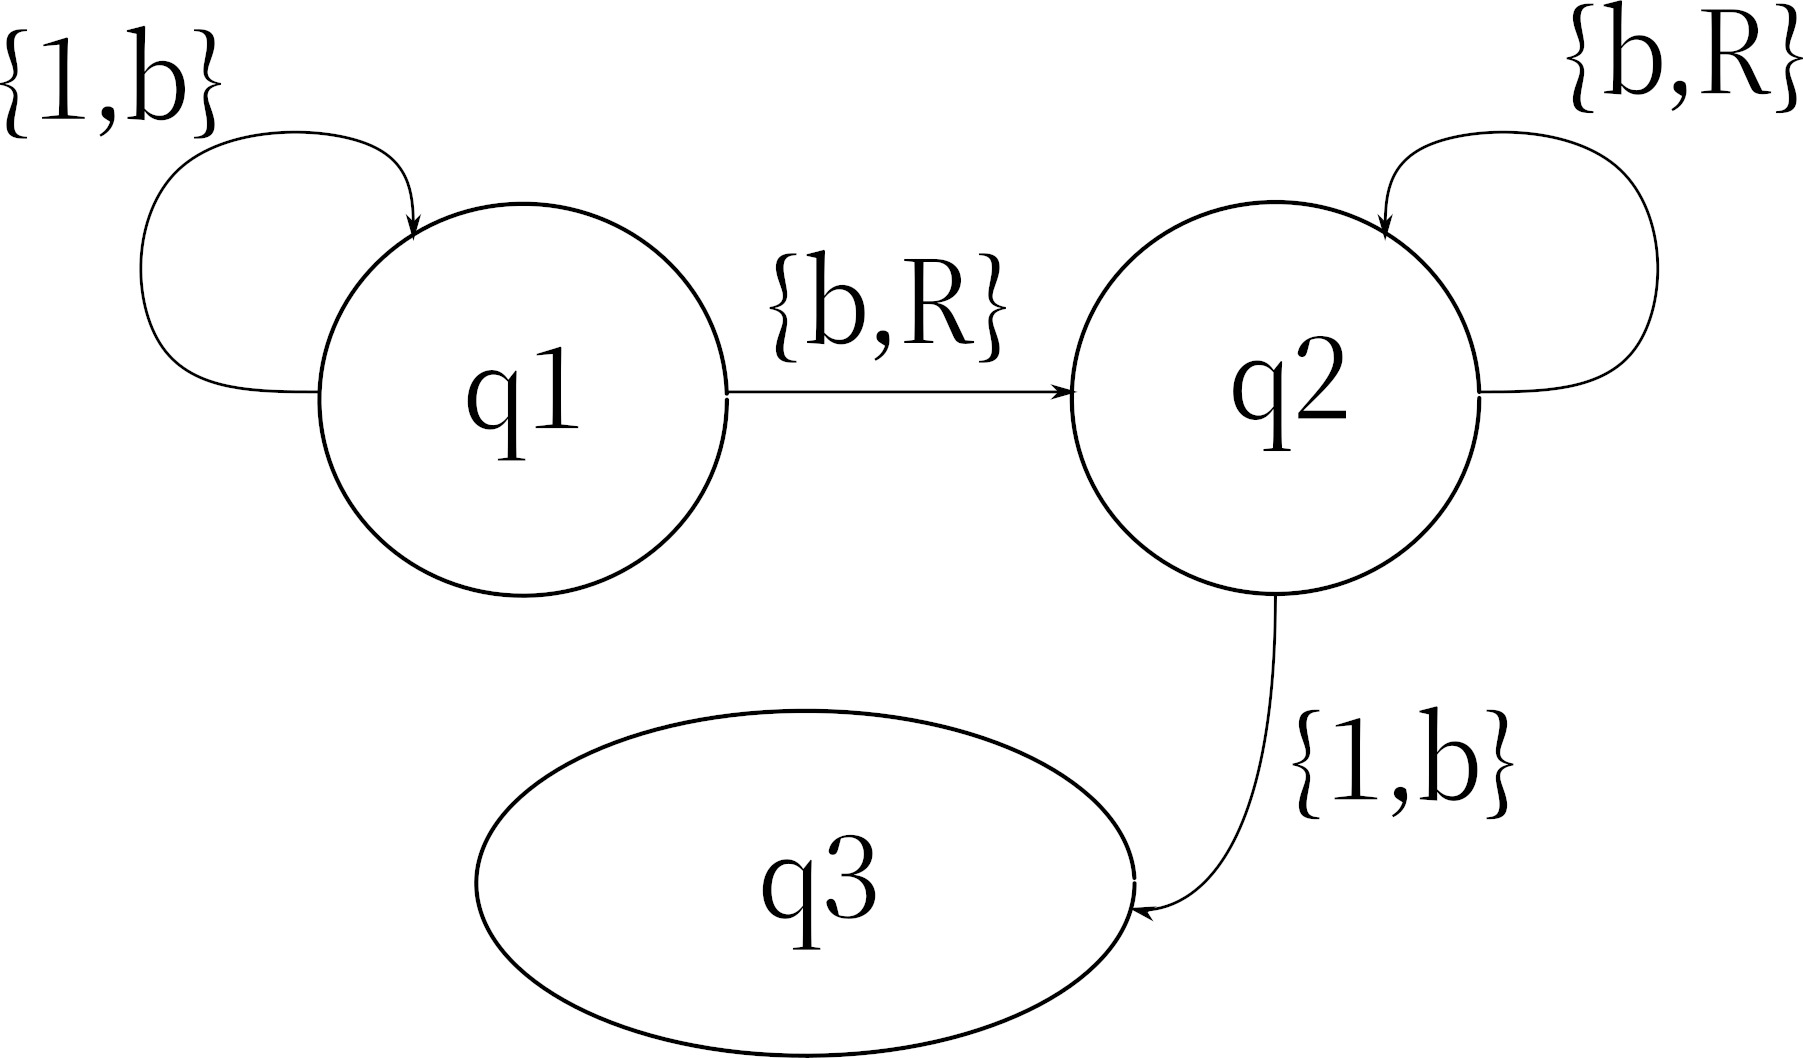
\includegraphics[ width=0.6\linewidth, height=\textheight, keepaspectratio]{./pics/mdtSomma.jpg}
    \caption{Grafo della macchina di Turing per le somme.}
    \label{fig:mdtSomma}
\end{figure}




\section{Altre versioni della macchina di Turing}

\subsection{Estensioni e menomazioni}

Una macchina di Turing può essere apparentemente potenziata mediante
l'estensione di essa tramite l'uso di \emph{nastri multitraccia}. In altre
parole, anziché adoperare un singolo nastro, si adoperano più nastri
simultaneamente. La macchina di Turing viene dunque espansa tramite l'aggiunta
di uno \emph{stato della memoria suppletiva}, che ci indica semplicemente il
numero del nastro dove la macchina di Turing sta agendo in quel momento.
Dunque, ci possiamo immaginare una macchina di Turing con tanti nastri e tante
testine che lavorano contemporaneamente, come illustrato in
Figura~\ref{fig:macchina-turing-multinastro}.

\begin{figure}[b]
    \centering
    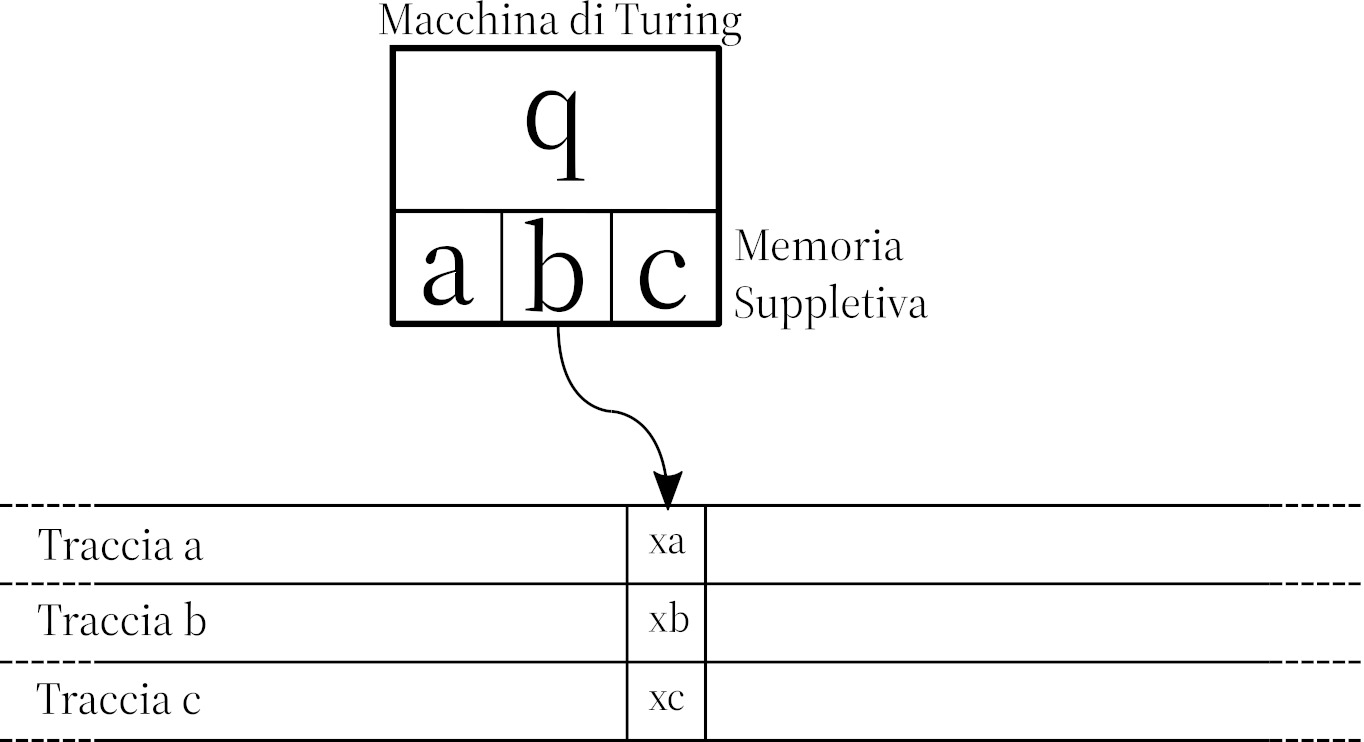
\includegraphics[ width=.8\linewidth, height=\textheight, keepaspectratio]{./pics/macchina-turing-multinastro.jpg}
    \caption{Macchina di Turing avente memoria con nastro multitraccia. La
    testina può collocarsi, una alla volta, su ciascuna delle nastre. La
memoria suppletiva rende possibile tenere traccia di quale nastro si sta
adoperando per l'esecuzione delle operazioni.}
    \label{fig:macchina-turing-multinastro}
\end{figure}

La domanda ora è se l'introduzione della multitraccia consenta di generare una
nuova macchina, con capacità di calcolo superiori a quelle della macchina di
Turing. La risposta è negativa: dal punto di vista della capacità computazione,
una macchina di Turing multinastro non aumenta né diminuisce le capacità. Una
macchina di Turing multinastro può essere implementata con un \emph{sistema
multitraccia} --- in altre parole, vengono adoperate \emph{tante testine quante
sono i nastri}. Ci si può facilmente ricondurre alla macchina di Turing
convenzionale semplicemente eliminando l'appena introdotto sistema multitraccia
e facendo agire la macchina su un nastro alla volta, o per meglio dire, una
macchina di Turing multitraccia può essere \textbf{simulata} da una macchina di
Turing convenzionale: essa dunque, non produce alcun tipo di miglioramento dal
punto di vista della computazione, cioè le due macchine hanno \textbf{la
stessa} potenza computazionale (Figura~\ref{fig:mdt-equivalenza-multitraccia}).
In parole povere, una macchina di Turing capace di agire su $N$ nastri
contemporaneamente può essere simulata (e quindi il suo funzionamento sarà lo
stesso) da $N$ macchine di Turing, ciascuna che agisce per conto proprio su uno
degli $N$ nastri.

Tale rappresentazione, tuttavia, può avere il vantaggio di presentare una
maggiore somiglianza con il tipo di computazione svolto all'interno di un
computer moderno. Si pensi infatti alla memoria RAM, alla memoria cache, al
disco rigido e così via; una macchina multinastro può ricalcare le varie memorie di un computer moderno. una macchina di Turing può dunque ``simulare''
qualsiasi computer moderno\footnote{Un computer può a sua volta simulare da una
macchina di Turing, dal momento che possono essere applicati potenzialmente
infiniti banchi di memoria al computer --- nella pratica, tuttavia, sappiamo
che ciò non è possibile, e i banchi di memoria non saranno mai del tutto
\emph{illmitati}. Sarebbe bello altrimenti!} semplicemente introducendo tanti nastri e tante tracce quante
sono quelle dei dispositivi fisici adoperati dal calcolatore moderno. Nella
fattispecie, si avrà un nastro ed una traccia per la memoria RAM, un altro
nastro ed un'altra traccia per la memoria a disco rigido, e così via. In
realtà, si tratta esclusivamente di un artificio che ci consente di tracciare
un collegamento fra il calcolatore moderno e la macchina di Turing, poiché una
macchina multinastro, sia essa multitraccia, può essere \emph{emulata} da una
macchina di Turing a nastro singolo. Quindi, anche se una macchina a nastro
singolo è più che sufficiente per calcolare qualsiasi funzione che è anche
calcolabile da un nostro computer moderno, possiamo adoperare l'astrazione del
multinastro per facilitarci nella comprensione e rendere il tutto più simile ad
un computer. Anche se poi la macchina di Turing lo surclassa comunque, essendo
dotata di \emph{memoria infinita} (mentre i nostri computer, no).

Il medesimo discorso si applica anche al primo tentativo di \emph{menomare} la
macchina di Turing (una sorta di sabotaggio), nel senso che potremmo pensare di
rendere il nastro semi-infinito, cioè illimitato solo a destra o solo a
sinistra. Ebbene, nonostante il sabotaggio venga messo in atto,
la macchina di Turing menomata avrà di fatto la medesima capacità
computazionale di quella ``standard'', perché possiamo sempre avere a
disposizione una quantità illimitata di memoria da un lato (un po' come per il
modello RAM), o far uso di trucchi come quello dell'alfabeto ausiliario
$\mathcal V$ che comunque faciliterebbero (di molto) le computazioni in una situazione
simile. Comunque la si veda, una macchina di Turing non si può né potenziare né
depotenziare, a meno di non effettuare operazioni che \emph{sconvolgano} il suo
funzionamento minandone le fondamenta, oppure rimuovendo l'ipotesi della
memoria illimitata da entrambi i lati (in quel caso si che si incapperebbe in
una limitazione pesante).

\begin{figure}[b]
    \centering
    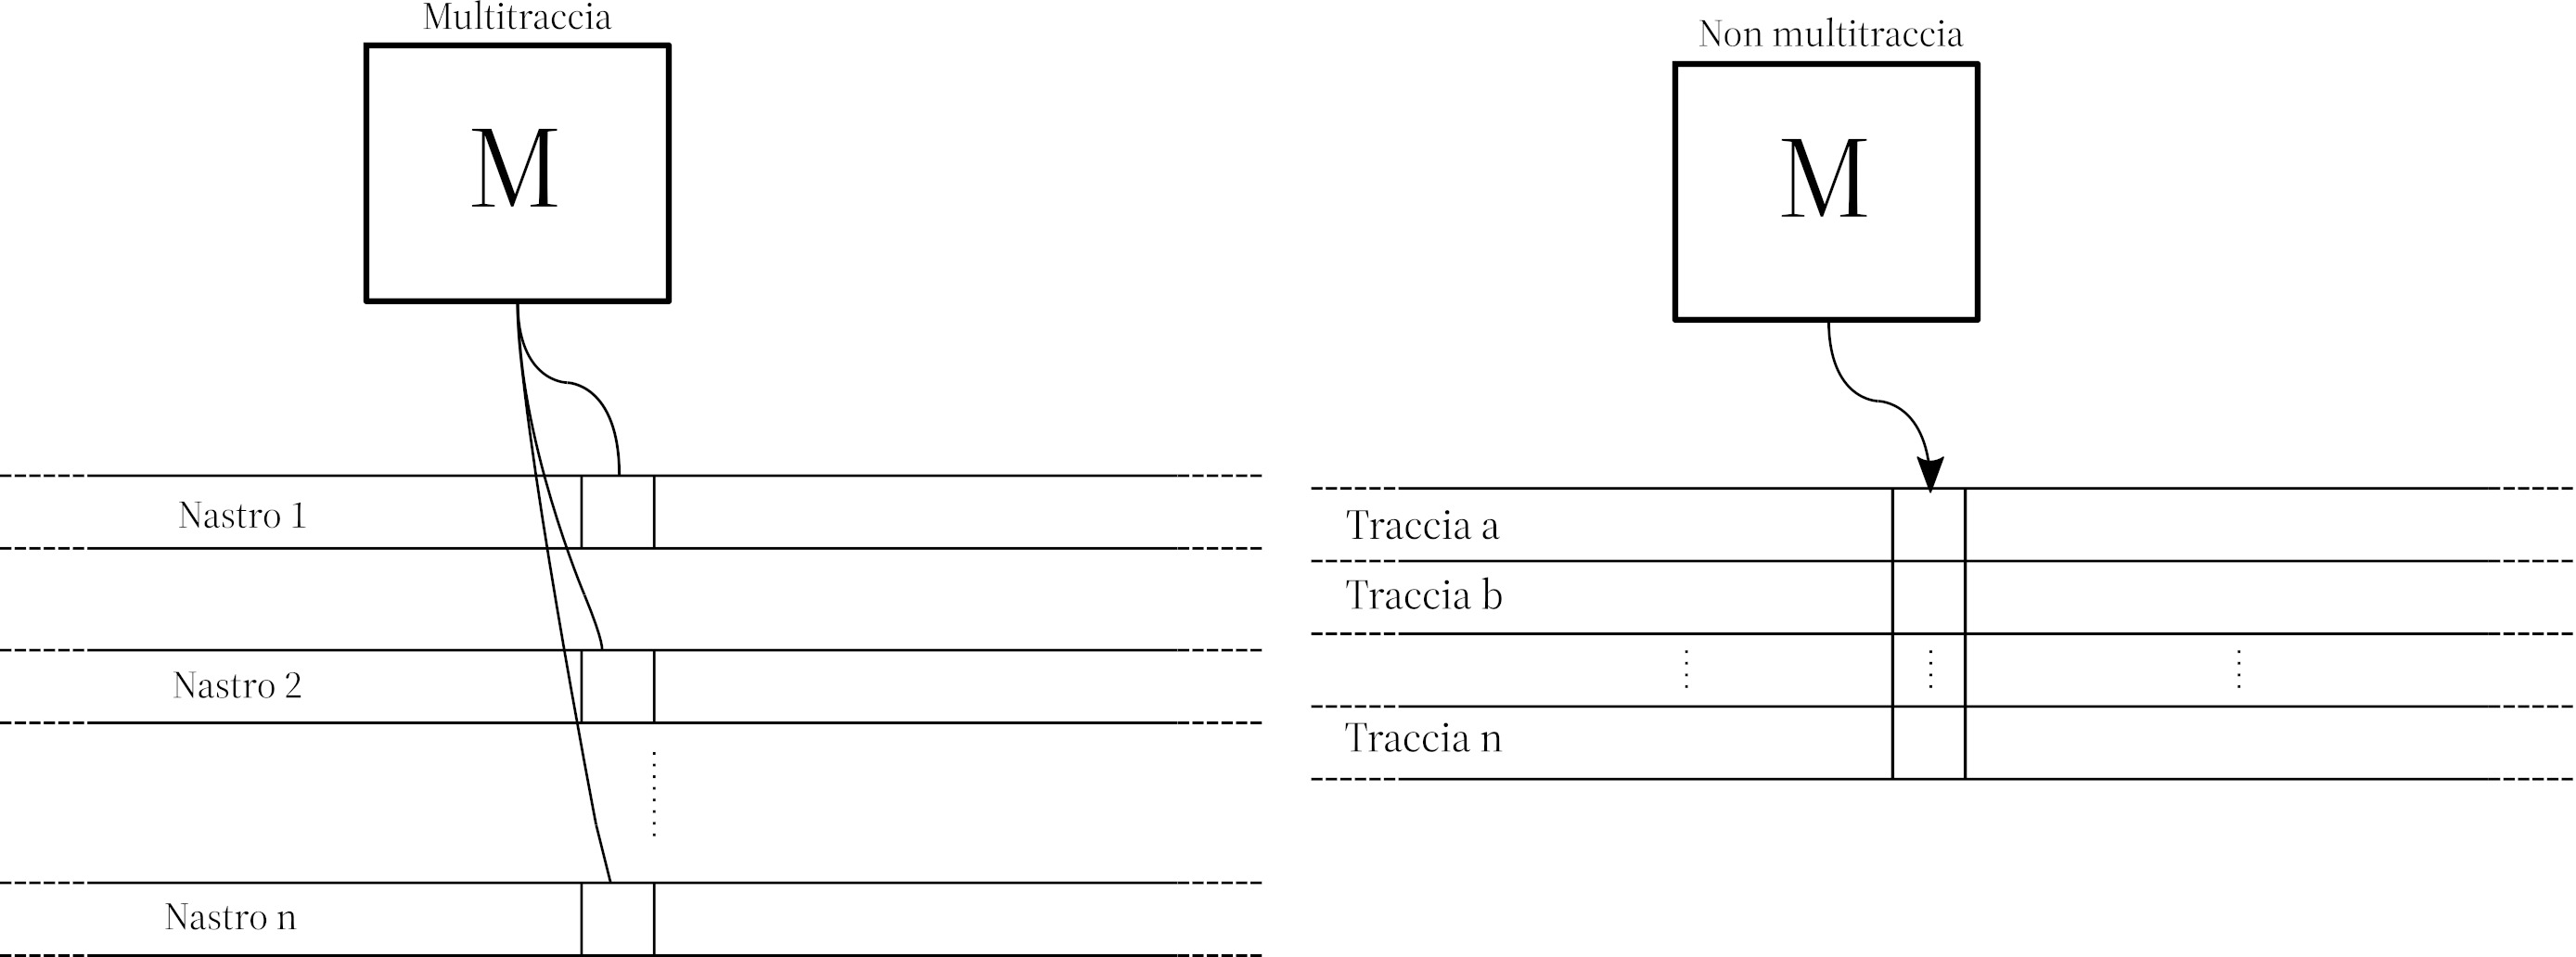
\includegraphics[ width=1.2\linewidth, height=\textheight, keepaspectratio]{./pics/mdt-equivalenza-multitraccia.jpg}
    \caption{Equivalenza fra una macchina di Turing a multitraccia e una
    macchina di Turing a singola testina. Non importa il numero di testine: la
macchina a singola testina potrà sempre percorrere (pazientemente) un nastro dopo l'altro,
simulando la macchina multitraccia.}
    \label{fig:mdt-equivalenza-multitraccia}
\end{figure}

\clearpage


\subsection{Macchina RAM per \emph{accettare} stringhe}

Uno dei possibili utilizzi per una macchina di Turing (o più in generale, per
una macchina Turing-equivalente) è quello di \emph{accettore} di stringhe: la
macchina riceve in ingresso un simbolo, una \emph{stringa}; essa si dirà
\emph{accettata} qualora la computazione risultante terminasse nello stato di
\textsc{Accettazione}, altrimenti si dirà \emph{rifiutata} qualora la
computazione terminasse invece in uno stato di \textsc{Rifiuto}. Per farla breve, essa ha come ``input''
(stato iniziale) una stringa, e l'evoluzione di questo input potrà portare o ad
uno stato in cui la stringa è considerata accettata, o in uno stato opposto in
cui essa è rifiutata. Si osservi che, in ogni caso, non c'è garanzia che una
macchina di Turing non possa ciclare all'infinito; in quel caso saremmo di
fronte ad una divergenza.

Nel modello RAM, per accettare una stringa è necessario operare una codifica.
In particolare, la stringa viene codificata in un numero naturale e la macchina
risponde con ``1'' o ``0'' a seconda che la stringa venga o meno accettata. In questo caso la codifica avviene sia per i valori di input, da stringa a numeri naturali, che per i valori finali della computazione, da numeri naturali ad accettato--rifiutato. Con
la macchina di Turing, invece, si può far intervenire direttamente uno
\emph{stato di accettazione} \textsc{Accettazione
} $q_Y$ o uno \emph{stato di
rifiuto} \textsc{Rifiuto } $q_N$. La
computazione terminerà qualora uno fra
questi due stati venisse raggiunto dalla macchina --- con conseguente
accettazione o rifiuto della stringa a seconda dello stato finale. Un'altra
possibilità è quella di accontentarci di \emph{semi-decidere} riguardo
l'accettazione di una stringa, cioè di dotarsi di una macchina in grado di
riconoscere sì la stringa in questione, ma di \emph{non poterla rifiutare},
poiché in tal caso vi sarebbe un'infinita computazione, una divergenza.

Lo stato iniziale viene di solito denotato con $q_0$, e potrebbero esserci degli
stati ulteriori ``intermedi'' fra quello iniziale e quelli terminanti. Un
esempio di accettazione è dato dalla macchina illustrata in
Figura~\ref{fig:mdtAccettazione1}. La macchina riconosce il linguaggio dato
dalle stringhe con due ``zeri'' nelle ultime due posizioni a destra, in
particolare essa riconosce tutte le stringhe che terminano con ``00''.

\begin{figure}[b]
    \centering
    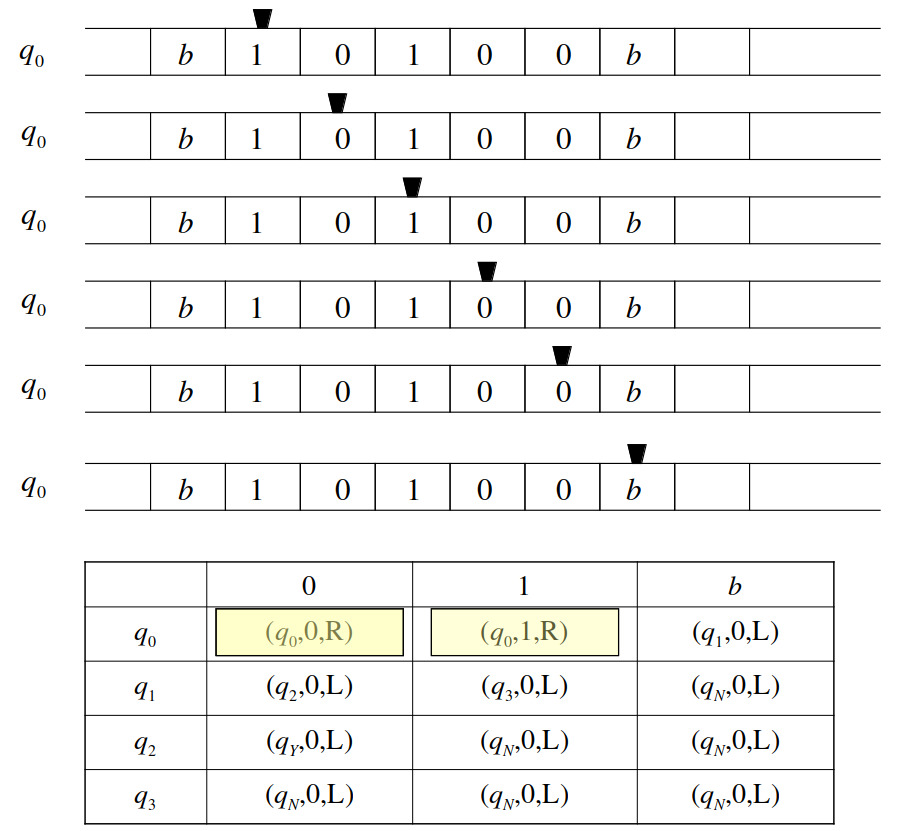
\includegraphics[ width=1.0\linewidth, height=\textheight, keepaspectratio]{./pics/mdtAccettazione1.jpg}
    \caption{Macchina che riconosce il linguaggio dato dalle stringhe con due $0$
nelle ultime due posizioni a destra, e suo funzionamento.}
    \label{fig:mdtAccettazione1}
\end{figure}

\clearpage

\subsection{Macchina di Turing definita a grafo}

Una macchina di Turing può anche essere ``definita a grafo''. In questo modello
di definizione, la macchina di Turing,
\begin{itemize}
    \item ha un \emph{nastro semi-illimitato} a destra, diviso in celle;
    \item ha un alfabeto $\Sigma$ accoppiato da un alfabeto \emph{ausiliario} $\mathcal V$;
    \item ha un simbolo di spaziatura $\Delta$, equivalente al simbolo
        \emph{blank} $b$;
    \item un puntatore, del tutto equivalente alla testina;
    \item un \emph{programma}, definito come \textbf{grafo finito orientato},
        con i vertici definiti come \emph{stato}. Vi è uno stato di inizio,
        indicato con \textsc{Inizio}, e un sottoinsieme eventualmente vuoto di
        stati di arresto, indicati con \textsc{Accettazione}. I nodi del grafo
        sono collegati da \emph{archi}.
\end{itemize}

Ciascun arco è della forma
\begin{figure}[h]
    \centering
    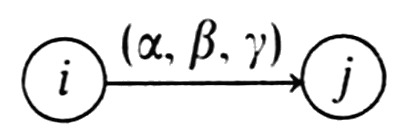
\includegraphics[ width=.4\linewidth, height=\textheight, keepaspectratio]{./pics/mdtGrafo.jpg}
    \label{fig:mdtGrago}
\end{figure}


dove $$\alpha \in \Sigma \cup \mathcal V \cup \{\Delta\}, \beta \in \Sigma \cup
\mathcal V \cup \{\Delta\} \mbox{ e } \gamma \in \{L, R\}.$$ Dunque, siamo
nello stato $i$; la macchina legge $\alpha$, scrive $\beta$ al posto di
$\alpha$, e infine va a destra oppure a sinistra a seconda che il simbolo
$\gamma$ sia pari ad $R$ o ad $L$. Una proprietà importante è che tutti gli
archi che partono da un medesimo vertice devono avere $\alpha$ diversi. Questo
perché la macchina non può tollerare delle ambiguità: leggendo un simbolo, può
compiere univocamente una sola azione, descritta dal grafo.

\begin{figure}[h]
    \centering
    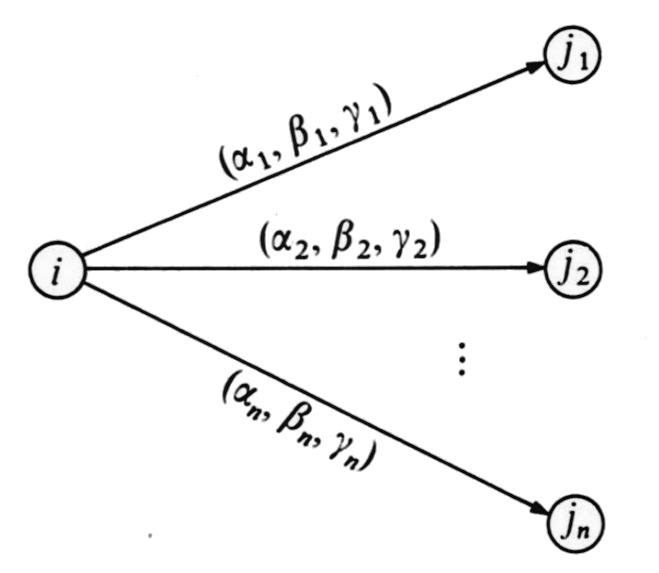
\includegraphics[ width=.4\linewidth, height=\textheight, keepaspectratio]{./pics/mdtArchiDiversi.jpg}
    \label{fig:mdtArchiDiversi}
\end{figure}

Se così non fosse, si avrebbero più cammini possibili per uno stesso
simbolo~--~un'ipotesi che come vedremo in seguito sarà violata assumendo che
una macchina di Turing possa non essere di tipo \emph{deterministico}.

\begin{figure}[b]
    \centering
    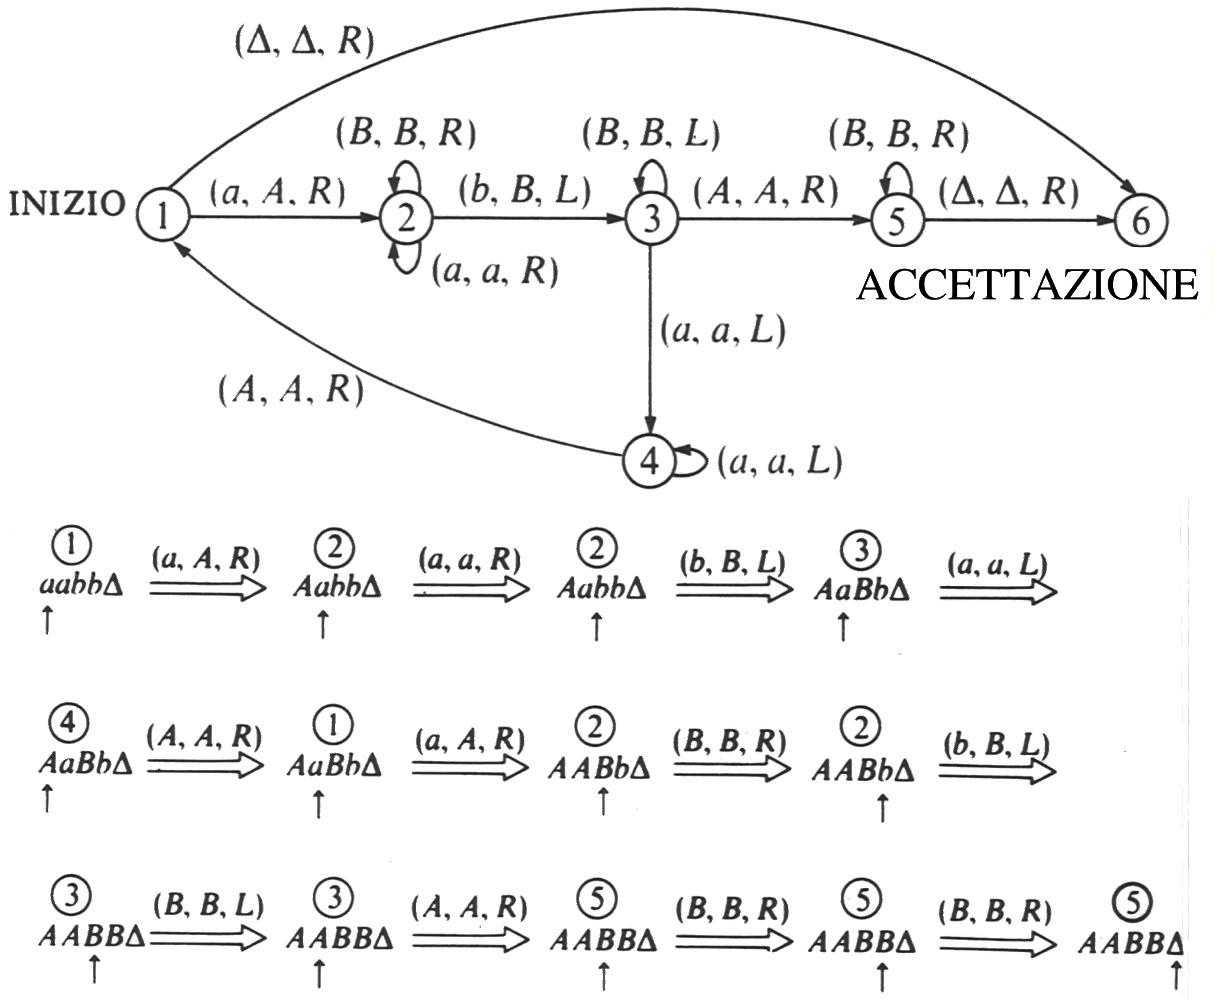
\includegraphics[ width=1.0\linewidth, height=\textheight, keepaspectratio]{./pics/mdtLetturaStringaSpeciale.jpg}
    \caption{Macchina di Turing in grado di riconoscere una stringa della forma
    $a^nb^n | n\geq 0$.}
    \label{fig:mdtLetturaStringaSpeciale}
\end{figure}

Si possono disegnare le macchine di Turing direttamente con i grafi, per poi
all'occorrenza convertirle nella forma a matrici di transizione. Il problema
espresso in Figura~\ref{fig:mdtLetturaStringaSpeciale} è il problema del
riconoscimento di una stringa avente forma $a^nb^n | n\geq 0$, ed è molto noto
nella teoria della computabilità, poiché è un tipico esempio di problema che è
risolubile da una macchina di Turing, ma \textbf{non risolubile} mediante una
\emph{macchina a stati finiti}. Tali macchine, infatti, non presentano alcun
tipo di \emph{memoria}, e dunque per questa particolare mancanza non sono in
grado di risolvere il problema del riconoscimento. La macchina di Turing,
invece, è in grado di risolverlo in virtù della sua superiore potenza di
computazione (e di memoria).

Un ulteriore esempio dell'applicazione della macchina di Turing a grafo è
mostrato in Figura~\ref{fig:mdtConcatenazioneStringhe}, dove la macchina in
questione è in grado di concatenare due stringhe a due lettere $a$ e $b$.

\begin{figure}[b]
    \centering
    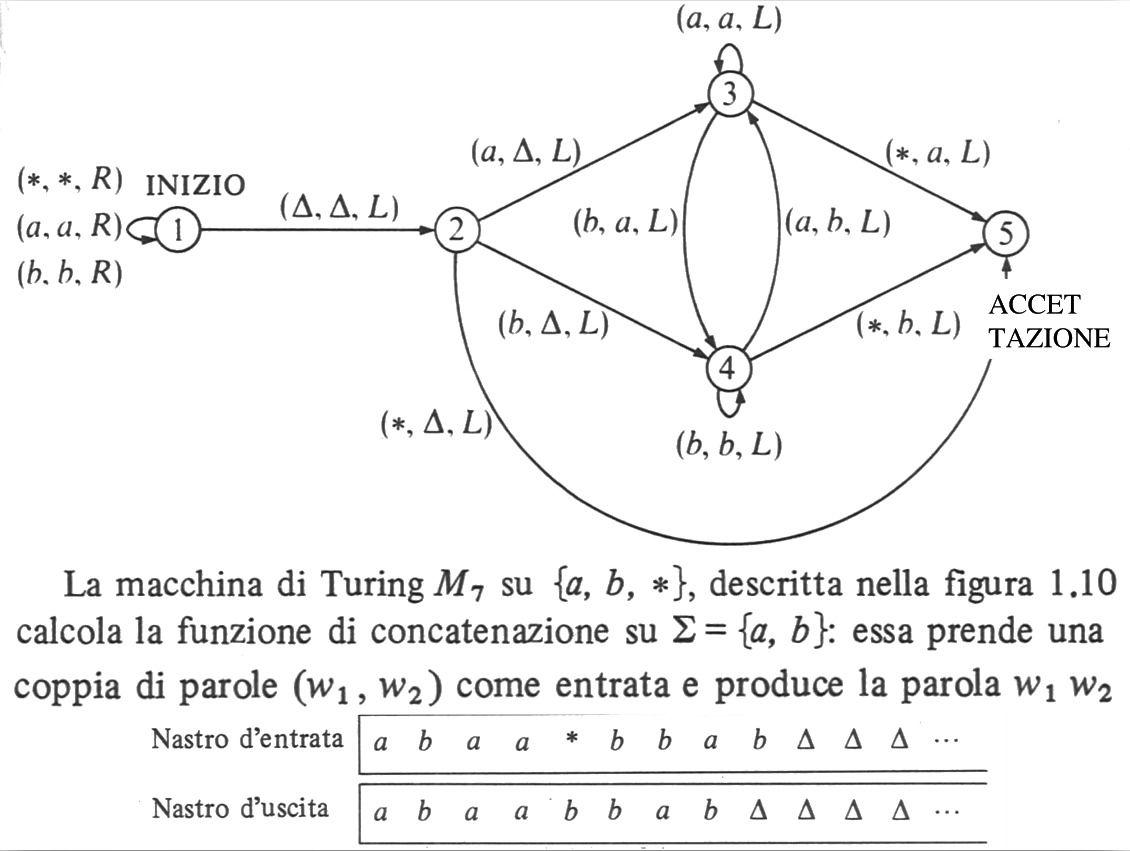
\includegraphics[ width=1.0\linewidth, height=\textheight, keepaspectratio]{./pics/mdtConcatenazioneStringhe.jpg}
    \caption{Macchina di Turing in grado di concatenare due stringhe $w_1$ e $w_2$.}
    \label{fig:mdtConcatenazioneStringhe}
\end{figure}



\chapter{Le macchine non deterministiche}

\section{Gerarchie delle potenze di calcolo}

Oltre alla macchina di Turing nelle sue varie versioni, sono possibili altre
tipologie di macchine, con vari livelli di gerarchia fra potenze di calcolo che
ne determinano le possibilità. Il seguente elenco ne illustra alcune, da minor
capacità di memoria a maggiore:

\begin{description}
    \item[macchine a \emph{stati finiti}] in questo caso, hanno $0$
        \emph{memorie push-down} --- le macchine a stati finiti sono le meno
        potenti in assoluto dal punto di vista computazionale, e non sono in
        grado di risolvere il problema del riconoscimento di stringhe $a^n
        b^n$, espresso in Figura~\ref{fig:mdtLetturaStringaSpeciale};
    \item[macchine a \emph{1 memoria push-down}] dotate di una memoria
        push-down che implementa una pila FIFO (\emph{first in----first out}),
        hanno una maggiore potenza di calcolo rispetto alla macchina a stati
        finiti;
    \item[macchine a \emph{2 memorie push-down}] dotate di $2$ memorie
        push-down, esse sono equivalenti alla macchina di Turing.
    \item[macchine \emph{di Post}] sono uno speciale tipo di macchine a memorie
        push-down, aventi una memoria di tipo LIFO (\emph{last in----first
        out}). Esse sono equivalenti alle macchine a $2$ memorie push-down e
        alle macchine di Turing;
    \item[macchine con 3 o più pile push-down] non forniscono vantaggi dal
        livello della potenza computazionale, e sono tutte Turing-equivalenti
        --- il vantaggio è, semmai, nella semplificazione di calcoli fornita
        dall'introduzione della pila aggiuntiva.
\end{description}


Perciò, la gerarchia delle potenze di calcolo è la seguente, dall'alto verso il basso:
\begin{enumerate}
    \item Macchine non deterministiche di Turing, con due memorie
        push-down~---~Macchine di Turing, Modello RAM, Macchine di Post,
        macchine finite con due memorie push-down (sono in grado di accettare
        $\{a^n b^n a^n| n \geq 0\}$). Si potrebbe dimostrare che le macchine di
        Turing deterministiche e non deterministiche hanno la medesima potenza
        di calcolo; 
    \item Macchine finite non deterministiche con una memoria push-down, sono
        in grado di riconoscere $\{w w^R | w\in\{a,b\}^*\}$\footnote{Il
        \emph{nodo di decisione} che introduce il non determinismo serve per
    gestire la situazione data dall'incapacità di riconoscere il punto di
rottura $ww^R$, cioè il punto in cui finisce $w$ ed inizia $w^R$. Con il non
determinismo, ogni qualvolta si arriva al nodo di decisione si tengono valide
entrambe le possibilità --- dunque, per questa ragione essa è più potente della
macchina ad una memoria push-down deterministica.};
    \item Macchine finite con una memoria push-down, riconoscono $\{a^n
        b^n|n\geq 0\}$;
    \item Macchine finite non deterministiche senza memorie push-down ---
        macchine finite senza memorie push-down --- automi finiti.
\end{enumerate}


\subsection{Alcune definizioni sulle stringhe}

Sia dato l'alfabeto $\Sigma^*$. Faremo uso di tre fondamentali funzioni
definite su $\Sigma^*$:
\begin{itemize}
    \item l'operazione \texttt{testa(x)}, che fornisce la ``testa'' di una stringa,
        ovverosia la lettera di estrema sinistra della parola $x$;
    \item l'operazione \texttt{coda(x)}, la quale invece fornisce la ``coda'' di una
        stringa, o la stringa privata della sua testa $x$;
    \item l'operazione $\sigma \cdot x$, che \emph{concatena} la lettera
        $\sigma$ e la parola $x$, per formare un'unica parola nuova.
\end{itemize}

Per esempio, se $\Sigma = \{a, b\}$, allora \texttt{testa(abb) = a}, \texttt{coda(abb) = bb} e inoltre $a \cdot bb = abb$.


\section{La macchina di Turing non deterministica}

La macchina di Turing effettiva è di tipo \emph{deterministico}. Nella
fattispecie, una macchina deterministica definita a grafo vede ciascun arco che
parte dallo stesso vertice avere \emph{simboli diversi}. Se ciò non fosse vero,
leggendo un unico simbolo $\alpha_i$ e trovandosi nello stato $q_j$ la macchina
di Turing non potrebbe ``scegliere'' il percorso, poiché ne esisterebbe più di
uno. Viceversa, una macchina \emph{non deterministica} rompe questa assunzione,
e permette alla macchina di compiere una scelta, sia essa arbitraria o del
tutto casuale, riguardo quale percorso seguire fra i vari disponibili. 

Il \emph{non determinismo} viene introdotto per due ragioni:
\begin{itemize}
    \item si desidera osservare se una macchina di Turing non deterministica
        sia più \emph{potente} oppure no di una macchina di Turing deterministica;
    \item si cerca di valutare se possano esistere differenti paradigmi di
        computazione (ad esempio, la computazione parallela è possibile?).
\end{itemize}

Una \emph{macchina di Turing non deterministica} può avere nel suo diagramma di
flusso dei \emph{nodi di decisione} dove a fronte di un medesimo simbolo vi
sono \emph{più archi possibili} --- il non determinismo viene dunque introdotto
da questo fenomeno: una macchina di Turing non deterministica può scegliere il
suo percorso con una legge non deterministica, ma semmai dettata dal caso o da
una \emph{scelta arbitraria}. È un po' come se la nostra macchina di Turing
fosse in grado di percorrere \emph{simultaneamente} tutti i percorsi possibili
descritti da un certo simbolo $\alpha_q$, poiché essa indiscriminatamente
accetta più archi alla lettura del medesimo simbolo $\alpha_q$, e può perciò
muoversi verso più nodi simultaneamente.

Una macchina non deterministica accetta l'idea che vi siano più possibilità di
sviluppo di una computazione a fronte di un medesimo simbolo identificato sul
nastro e associato ad un determinato stato; sono dunque possibili diversi
percorsi di computazione. Questo tipo di macchina, ad esempio, potrebbe
percorrere \emph{tutti i percorsi simultaneamente}, concependo il
\textbf{parallelismo} nella computazione, nel senso che più possibilità e
percorsi nel calcolo sono possibili. 

Questa nuova potenzialità, apparentemente di
gran lunga migliorativa, \textbf{non aumenta} la potenza di calcolo della
macchina di Turing. Questo perché una macchina di Turing deterministica è in grado, in linea di principio, di
simulare una macchina non deterministica. Per convincersi di ciò è sufficiente
compiere una ricerca per ogni diramazione dell'albero dei nodi, con un aumento
esponenziale\footnote{L'aumento esponenziale è dovuto al fatto che, ad ogni
diramazione effettuata da una macchina di Turing non deterministica, la
relativa macchina deterministica dovrà (almeno) sdoppiarsi su $2$ percorsi.}
del numero di operazioni da effettuare, ma pur sempre un'operazione
realizzabile e computabile da una macchina di Turing. In altre parole, armata
di una certa pazienza, la macchina di Turing deterministica può percorrere uno
alla volta ciascuno dei sentieri che la sua controparte non deterministica
avrebbe percorso tutti contemporaneamente. Una macchina non deterministica ha
dunque il potenziale vantaggio di poter risolvere problemi in \emph{tempo
lineare} che dalla macchina deterministica sarebbero invece risolti in in tempo
esponenziale. Una grandissima spinta della velocità di calcolo, ma che non
garantisce di calcolare nulla di più di quanto si potrebbe fare con una
macchina di Turing deterministica. Resta da domandarsi se ciò renda in qualche
modo possibile rendere più efficienti i nostri computer. Ebbene, una macchina
di Turing non deterministica può essere vista come una macchina di Turing
deterministica ove, ad ogni diramazione, \emph{lancia la computazione di nuove
macchine di Turing}. Se una macchina di Turing deterministica deve seguire 3
nuovi percorsi a partire da un certo nodo, essa è come se accendesse 3 nuove
macchine di Turing, ciascuna su uno dei 3 percorsi e che calcola per conto
proprio. È chiaro che questo procedimento di lancio di nuove macchine può
essere, nella nostra immaginazione, arbitrariamente effettuato senza poter
incappare in qualche limitazione, accendendo di volta in volta sempre nuove macchine senza mai porre un limite al loro numero. Nella realtà materiale (purtroppo) ciò
equivarrebbe a lanciare \emph{un nuovo computer} ad ogni diramazione. Questo è
realizzabile fino ad un certo punto (ammesso di disporre di tanti computer), ma
è chiaro che il procedimento non può essere arbitrariamente replicato. Siccome
i nostri computer sono dotati di core, possono raggiungere (da soli) buone
capacità di parallelizzazione, ma infinitamente inferiori a quelle richieste
per una vera parallelizzazione e per simulare il non determinismo dal punto di
vista della velocità di calcolo (gli infiniti core non esistono). Se ciò fosse
invece possibile nel mondo materiale, potremmo effettivamente risolvere
problemi difficilmente trattabili in tempo polinomiale, rendendoli di fatto
trattabili.

Il parallelismo è insito nella macchina non deterministica;
supponendo di voler risolvere un problema di accettazione, la stringa si
considera \emph{accettata} qualora uno qualunque fra i percorsi possibili
incappasse nello stato di \textsc{Accettazione}. Più nello specifico, una parola $w \in \Sigma^*$ si
dice \emph{accettata} da una macchina di Turing non deterministica se esiste
una computazione della macchina $M$ che cominci con entrata $x=w$, e che
termini ad un arresto con lo stato di \textsc{Accettazione}. Se $w$ non viene
accettata e lo stato di arresto è quello del \textsc{Rifiuto}, allora si dice
che $w$ è \emph{rifiutata}. In alternativa, siamo di fronte ad un ciclo
infinito $w \in ciclo(M)$, cioè dinanzi ad una divergenza.

\begin{figure}[ht]
    \centering
    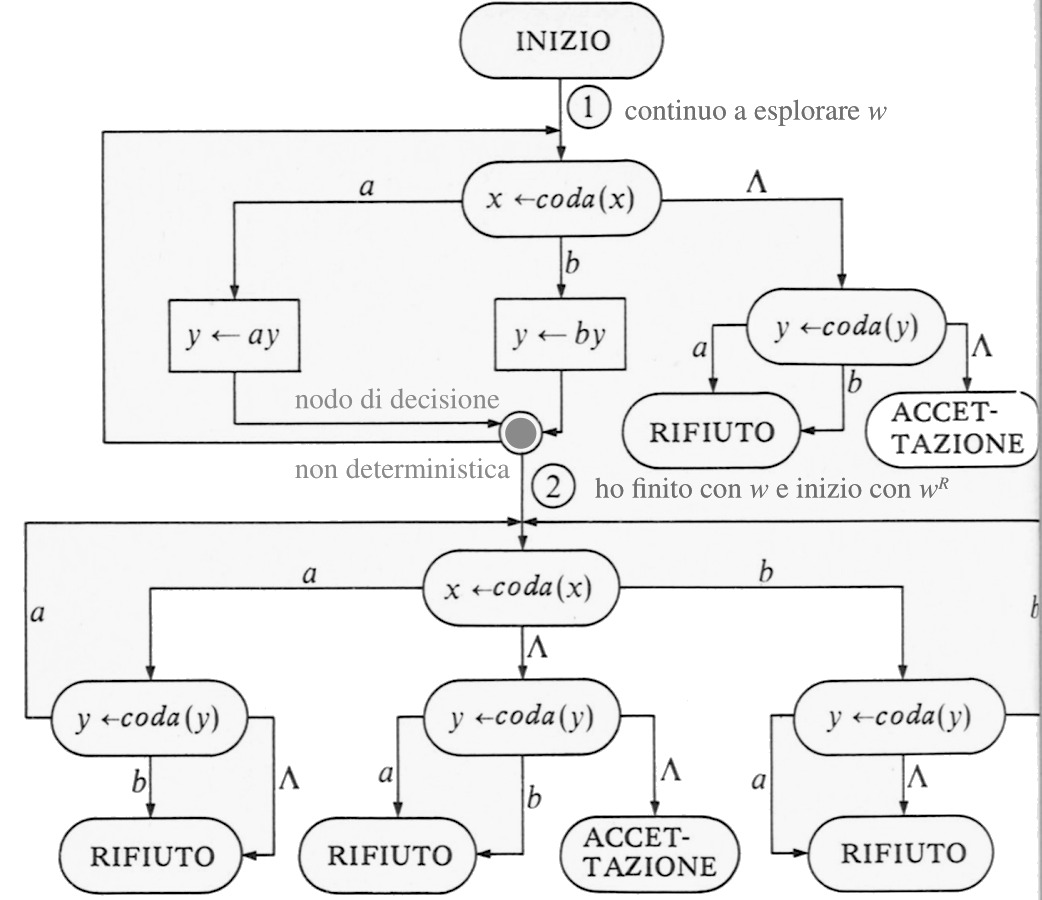
\includegraphics[ width=1.0\linewidth, height=\textheight, keepaspectratio]{./pics/accettoreWWR.jpg}
    \caption{Macchina finita non deterministica che accetta le stringhe del
    tipo $\{w w^R | w\in\{a,b\}^*\}$. Questa macchina accetta tutte le stringhe
di quel tipo, e rifiuta tutte le altre $\Sigma^* - \mbox{accettazione}(M_6)$.
Esempi di stringhe accettate sono la stringa vuota $\Delta$, $aa$, $babbab$,
$bbbabbabbb$ e così via.}
    \label{fig:accettoreWWR}
\end{figure}



Possiamo quindi pensare ad una macchina di Turing non deterministica
come ad una macchina avente per ogni cella, nella matrice di transizione, un
\emph{insieme} $\delta(q,s)$ di triple $q_i, s_i, \alpha_i$, dove $\alpha_i \in
\{L,R\}$ e ad ogni elemento dell'insieme corrisponde una possibile scelta da
compiere arbitrariamente o casualmente; dunque da lì è ottenuto il non
determinismo della macchina. Ogni possibile scelta genererà un diverso ramo
nell'albero della computazione; per l'accettazione di un simbolo è
sufficiente che uno \emph{qualsiasi} fra i rami di computazione termini nello
stato di \textsc{Accettazione}. Dunque, benché una macchina di Turing non
deterministica non \textbf{aumenti} la potenza di calcolo intrinseca della
macchina, essa consente la \textbf{parallelizzazione} dei possibili percorsi
della computazione, rendendo di fatto possibile risolvere in tempo lineare
problemi che sarebbero risolubili comunque, ma in tempo esponenziale, per una
macchina deterministica.

\subsection{Equivalenza fra macchine non deterministiche e macchine multinastro}

\begin{thm}
    Ogni macchina di Turing non deterministica ha un equivalente macchina di
    Turing deterministica multinastro.
\end{thm}

\textsc{Dimostrazione} --- Una traccia della dimostrazione è una ricerca
nell'albero di computazione. Con almeno due nastri, si simula con uno la
macchina non deterministica mentre con l'altro si collezionano tutti i
possibili $k$ ``prossimi passi'' della tabella di transizione. La macchina di
Turing deterministica allora controllerà tutte le configurazioni
stato--simbolo, livello per livello, dell'albero di computazione. Lo stato
finale di \textsc{Accettazione } terminerà la computazione complessiva.

\begin{flushright}
$\blacksquare$
\end{flushright}

L'idea è quella, dunque, di \emph{simulare} il non determinismo compiendo un
numero crescente in modo esponenziale di passi, uno per ogni ramo dell'albero
non deterministico di computazione.

\begin{thm}
    Ogni macchina di Turing non deterministica $T_M(n)$ ha un equivalente
    macchina di Turing deterministica con ordine $2^{O(T_M(n))}$.
\end{thm}

\textsc{Dimostrazione} --- Una traccia può essere che il numero massimo di
foglie è $O(b^{T_M(n)})$, dove $b$ è il numero di figli. Il tempo per viaggiare
dalla radice lungo ogni ramo è, per una macchina multinastro,
$$O(T_M(n)b^{T_M(n)}) = 2^{O(T_M(n))},$$ mentre per una macchina a nastro
singolo $$(2^{O(T_M(n))})^2 = 2^{O(2T_M(n))} = 2^{O(T_M(n))},$$ dunque l'ordine
è lo stesso.
\begin{flushright}
$\blacksquare$
\end{flushright}


\begin{figure}[h]
    \centering
    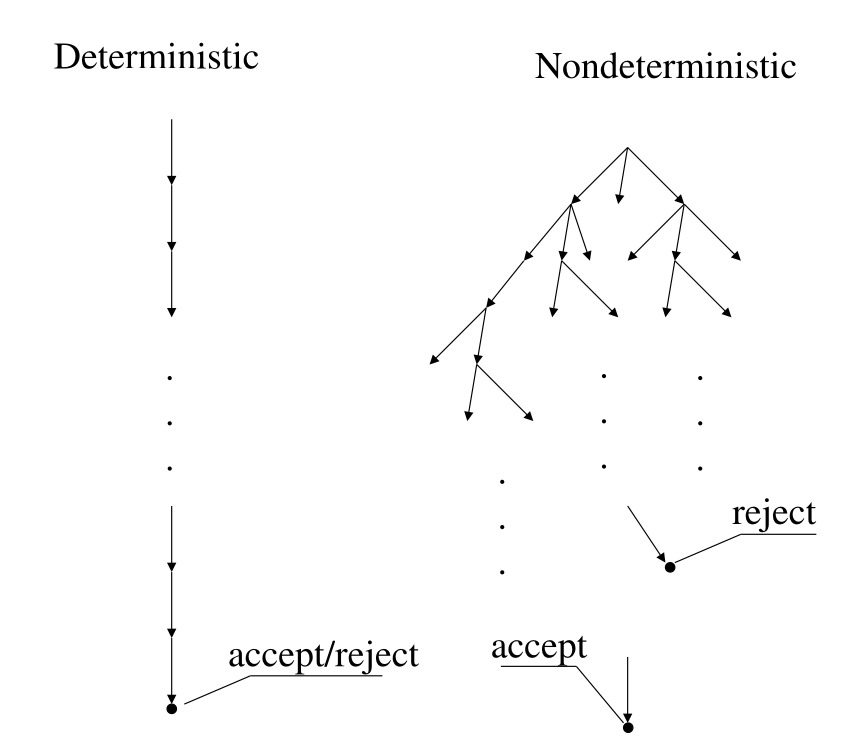
\includegraphics[ width=1.0\linewidth, height=\textheight, keepaspectratio]{./pics/ndtmEsempio.jpg}
    \caption{Esempio di computazione ``in parallelo'' effettuata dalla macchina
    non deterministica (a destra), e simulazione da parte della macchina
deterministica (a sinistra).}
    \label{fig:ndtmEsempio}
\end{figure}



\chapter{Le reti neuronali di Hopfield}

Le \textbf{reti neuronali} incarnano un diverso paradigma di computazione
rispetto a quello della computazione procedurale algoritmica. Storicamente esse
prendono spunto dalla natura, in particolare dal concetto di \emph{neurone},
inteso come singola unità di calcolo, dotata di input, di output e di una
\emph{funzione caratteristica}. Diversamente dall'idea della computazione
procedurale, dove la \emph{complessità} è definita tramite la complessità di
tipo computazionale (o temporale), le reti neuronali esprimono la loro
complessità attraverso la \textbf{complessità strutturale}, o
\textbf{complessità circuitale}. In altre parole, per risolvere un problema
l'idea è quella di aumentare la complessità di tipo circuitale della rete, ad
esempio aggiungendo neuroni, facendo variare le conduttanze, adoperando diverse
funzioni di attivazione. La computazione è di tipo \emph{collettivo}, ed emerge
come proprietà dell'\emph{evoluzione dinamica} della rete. Ogni decisore
locale, detto \emph{neurone}, non ha visibilità della computazione globale, e
svolge il proprio compito localmente --- ogni decisore locale concorre alla
soluzione globale in modo sfumato, con il proprio valore in stato alto o basso:
la rete è \textbf{robusta} rispetto a malfunzionamenti locali, poiché ciascun
neurone singolo non è critico e non può pregiudicare l'intera rete da solo.
Spesso è addirittura possibile eliminare qualche neurone senza che la rete ne
risenta in maniera rilevante.

Dal punto di vista strettamente logico, il paradigma di computazione a reti
neuronali è l'unico paradigma radicalmente differente da quello procedurale,
mentre il paradigma \emph{a DNA}\footnote{Trattasi di un
paradigma di calcolo dove si va a cercare lo spazio delle soluzioni tramite una
vera e propria ricerca esauriente, e si catturano quelle più adatte.  La
potenza di questo metodo è quello di potersi permettere una ricerca esauriente
della soluzione, poiché ciascun DNA è infinitesimamente piccolo, e dunque può
essere esaminato in parallelo.} è una tipologia di calcolo che, nella realtà,
non differisce sostanzialmente dal metodo procedurale.

Esistono due filoni di reti neuronali; il primo associato ai
\textbf{perceptron}, macchine a strati che fungono da riconoscitori di pattern
e configurazioni. Le variabili di ingresso rappresentano un ente, una
configurazione del sistema esterno, e il perceptron è in grado di fornire in
output una risposta che consente di riconoscere tale configurazione o pattern
in base a come essa sia stata configurata e ai suoi parametri. I
cosiddetti \emph{multilayer perceptron} sono particolari casi di perceptron,
aventi i neuroni organizzati in \emph{layer}. Vi sono due layer ``principali''
di input e di output, e dei layer ``nascosti'' (in gergo \emph{hidden layer})
dove avvengono ulteriori passaggi intermedi. Tipicamente, i layer sono
costituiti da neuroni aventi particolari \emph{funzioni di attivazione}. Le
funzioni di attivazione sono ciò che determina il comportamento dei singoli
neuroni --- in particolare, esse determinano la maniera in cui un neurone debba
attivarsi o rimanere nello stato di quiete. I perceptron hanno la
caratteristica fondamentale di essere \emph{feed-forward}, cioè di avere una
\emph{direzionalità} nella rete: i neuroni non possono essere connessi in
cicli, cioè il corrispondente grafo è aciclico. L'infrastruttura dei perceptron
ha un comportamento di tipo euristico, cioè non esiste alcun modello di
computazione associato alla struttura, non vi sono teoremi e, di fatto, il
tutto è carente di un solido un apparato matematico. Per modellare un
perceptron, solitamente, si adottano tecniche euristiche di \emph{machine
learning}, con apprendimenti automatici.

Il secondo filone, invece, è quello della \textbf{rete di Hopfield}; tale filone
sarebbe in grado, in linea di principio, di \emph{risolvere problemi} di
natura matematica. Mediante una rete di Hopfield è possibile risolvere ad
esempio il \emph{travelling salesman problem}, un problema presumibilmente
intrattabile\footnote{``Presumibilmente'' si riferisce al fatto che, fino ad
ora, nessuno è riuscito a dimostrare né che tale problema può essere risolto in
tempo polinomiale, né che non può esserlo.}. Le reti di Hopfield, diversamente
dai perceptron, possono essere modellate con grafi ciclici, dunque esistono
percorsi ciclici fra neuroni.

Ambedue i modelli, tuttavia, non possono essere considerati dei veri e propri
modelli alternativi a quello della macchina di Turing; in primis per l'assenza
dell'apparato matematico, e in secondo luogo poiché è stato dimostrato che
nella sostanza e sotto opportune ipotesi una rete neurale ha la stessa potenza
di calcolo del modello RAM. Le reti neurali quindi, non sono un modello di
computazione alternativo, semmai sono un \emph{paradigma} differente.

Le reti neuronali hanno avuto grande successo in $3$ periodi storici:
\begin{itemize}
    \item all'inizio degli anni $40$ --- nel $1948$ fu fornito il primo modello
        di neurone e rete neuronale. L'idea fu quella di avvalersi di una
        macchina fisica per simulare il comportamento dei neuroni naturali,
        presenti nel nostro cervello
        (Figura~\ref{fig:retiHopfieldNeuroneParagone}. All'epoca uscirono anche
        articoli su memorie a breve e lungo termine adoperando reti neuronali;
    \item durante gli anni $80$ --- nei primi anni $80$, Hopfield individuò un
        modello di reti neuronali che associava le reti neuronali ad un
        particolare modello matematico; qualità che prima era assente. Si
        tratta di una caratteristica fondamentale: quando si cerca di risolvere
        problemi con le reti neuronali, l'assenza di teoremi (ad esempio,
        quelli asintotici) non ci permette di stabilire la \emph{qualità} di
        una soluzione, oppure se la computazione andrà in qualche maniera a
        buon fine. Dunque, l'assenza di un buon apparato matematico che faccia
        da base alle reti neuronali è il principale svantaggio di tale
        paradigma. Hopfield riuscì a fornire la soluzione di alcuni fra questi
        problemi matematici, suggerendo la possibilità di risolvere problemi,
        come ad esempio quello sopra citato del \emph{travelling salesman
        problem}. Ci fu allora una corsa dal punto di vista scientifico
        riguardo la possibilità di risolvere in maniera efficiente i problemi
        presumibilmente intrattabili. Si può dimostrare, tuttavia, che la
        potenza di computazione di una macchina di Hopfield \textbf{non è
        superiore} alla capacità di computazione della macchina di Turing. Con
        una macchina di Hopfield non è dunque possibile risolvere in tempo
        polinomiale problemi che non sono risolubili in tale maniera già dalla
        macchina di Turing --- vi è dunque l'\emph{equivalenza} fra le due
        macchine. Le reti di Hopfield caddero pertanto ben presto in disuso;
    \item il terzo ed ultimo periodo d'oro delle reti neuronali è il giorno
        d'oggi, dove la potenza di calcolo superiore delle macchine moderne
        apre la strada ad un ampio uso delle reti neuronali in applicazioni
        concrete, che si avvalgono della pura potenza computazionale di gran
        lunga maggiore rispetto al passato per produrre risultati in tempo
        apprezzabile. Esse si vedono applicate in problemi di machine learning
        quali il riconoscimento di pattern in immagine, la classificazione di
        immagini, l'estrazione di feature (per il loro utilizzo con ulteriori
        tecniche di machine learning).
\end{itemize}

\begin{figure}[ht]
    \centering
    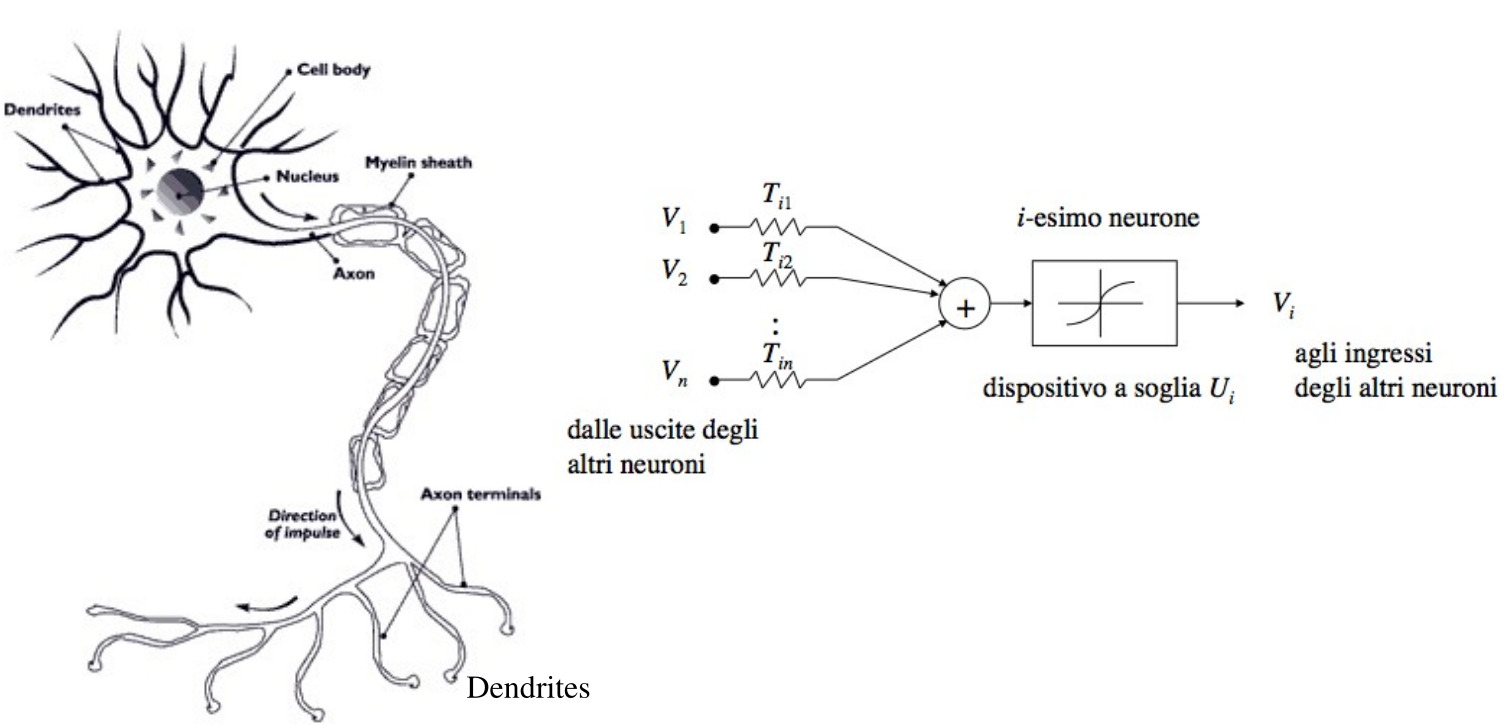
\includegraphics[ width=1.0\linewidth, height=\textheight, keepaspectratio]{./pics/retiHopfieldNeuroneParagone.jpg}
    \caption{Paragone fra neurone naturale e neurone di Hopfield. Si osservino
    innanzitutto le somiglianze fra le due strutture. La somiglianza principale
è il fatto che anche i neuroni naturali presentano vari input e vari output,
collegati con diversi altri neuroni. Tipicamente, anche un neurone naturale
presenta una vera e propria funzione di attivazione, che ne determina il
comportamento ``a soglia''. La stimolazione del neurone naturale è stimolata da
segnali continui, sebbene il \emph{firing} (eccitazione del neurone) avvenga in
maniera discreta.}
    \label{fig:retiHopfieldNeuroneParagone}
\end{figure}



\section{Il neurone reale ed il neurone simulato}

Una macchina di Hopfield simula un neurone reale. Vi sono all'incirca $10^{11}$
neuroni (cento miliardi) nel cervello, i quali formano una rete neuronale di
una complessità strabiliante. Il cervello è in grado di svolgere una quantità di
compiti enorme, in modo molto efficiente --- il cervello è infatti la struttura più
complessa che esista nell'universo noto, non paragonabile ad alcun altro tipo
di struttura, sia essa già esistente in natura o creata artificialmente. I
segnali elettrici nel cervello si sviluppano nell'ambito dei \emph{segnali
continui}, tuttavia il funzionamento di un neurone si svolge, in realtà, 
propriamente nell'ambito dei \emph{segnali discreti}. Vi sono infatti i
cosiddetti \emph{spike}: un neurone si ``eccita'' o si ``rilassa'',
manifestando dunque un comportamento discreto secondo questo punto di vista,
anche se il sottostante segnale è, di fatto, un segnale elettrochimico di
natura continua.

\section{La rete discreta di Hopfield}

La \textbf{rete discreta di Hopfield} è composta da singoli neuroni, modellati tramite
le tensioni elettriche. Ciascun $i$-esimo neurone ha la forma illustrata in
Figura~\ref{fig:retiHopfieldNeuroneParagone}: esso è dotato di $n$ ingressi
$V_j$ collegati ad altri neuroni, delle ``conduttanze'' dal valore $T_{i,j}$
che simulano i contatti fra neuroni\footnote{Il valore di tali conduttanze
\emph{varia} in funzione del tempo, in particolare in base a quanto
frequentemente il neurone viene sollecitato --- questo modello artificiale è
basato su quello reale, dove i dendriti variano a seconda della frequenza con
cui il neurone viene sollecitato.}; ciascuno degli ingressi si sommerà e la
somma verrà valutata dalla \emph{funzione di attivazione}, collocata nella
parte centrale. Il neurone di Hopfield è un dispositivo dal comportamento
\emph{a soglia} (sigmoide): la funzione di attivazione pesa la somma degli
ingressi, producendo un output $V_{i}$ \textbf{pressoché discreto} da dirigere
agli ingressi di altri neuroni. Nel caso discreto, la soglia si dice essere
\emph{rigida}: stabilita la soglia $U_i$ del neurone, avremo due possibilità,
\begin{itemize}
    \item o $V_{i} = 1$ se $\sum_{j\neq i} T_{ij} V_j > U_i$;
    \item oppure $V_{i} = 0$ se $\sum_{j\neq i} T_{ij} V_j < U_i$;
\end{itemize}

cioè la soglia determina il comportamento che l'uscita del neurone presenta a
seconda dei valori dell'ingresso (o più precisamente, a seconda di quanto vale
la loro somma pesata dalle conduttanze $T_{ij}$).

In un certo senso quindi, si può affermare che un neurone di Hopfield si
comporta ``discretamente'', nel senso che il suo valore di uscita può assumere
valori o prossimi allo $0$, o prossimi all'$1$, con possibili valori intermedi
dipendenti esclusivamente dalla forma che la funzione di attivazione presenta
(si assume che essa difficilmente possa avere la forma di un perfetto gradino,
e che esistano porzioni di essa in cui il valore è compreso fra $0$ ed $1$ con
valori continui. Ciononostante, è sufficiente interpretare il segnale continuo
in senso discreto, cioè valutando con un'opportuna soglia il valore dell'output
di un neurone, un po' come avviene nei circuiti digitali). Nella fattispecie,
consideriamo un comportamento a soglia di tipo ideale, cioè nel quale la
funzione di attivazione è un gradino ideale.

Per quanto concerne le reti di Hopfield, è importante fare due osservazioni. La
prima è che se $V_i = 1$, in ogni caso (sia che fosse già in $1$ o che fosse in
$0$) si ha che $\Delta V_i \geq 0$. Viceversa, se $V_i = 0$, in ogni caso si
avrà che $\Delta V_i \leq 0$: questa cruciale osservazione ci permette di
stabilire che

$$\Delta E = -\Delta V_i (\sum_{j \neq i} T_{ij}V_j - U_i) \leq 0,$$ cioè la
variazione di energia, ovvero la potenza, \emph{è sempre minore di zero}. La
\textbf{variazione dell'energia della rete}, dunque, \textbf{è sempre
negativa}. Questo fatto è di fondamentale interesse, poiché ci definisce la
maniera in cui la rete tende ad evolversi, riducendo ad ogni passo la quantità
di energia totale.

La seconda importante osservazione è che nel caso in cui si assuma una
simmetria della rete (cioè quando il neurome $i$-esimo incide sul neurone
$j$-esimo tanto quanto il neurone $j$-esimo incide su quello $i$-esimo),
l'energia $E_i$ del neurone $i$-esimo sarà pari a

$$E_i = -V_i(\sum_{j\neq i} T_{ij}V_{j} - U_i),$$ e sotto ipotesi $T_{ij} =
T_{ji}$, si ha infine che l'\textbf{energia della rete di Hopfield} $E$ è pari
a

\begin{equation}
    E = -\frac{1}{2} \sum_{ij, j\neq i} T_{ij}V_i V_j + \sum_{i} V_i U_i,
\end{equation}

un termine corrispondente ad una \emph{forma quadratica}.

Dunque, per come è stata impostata la rete e per le due osservazioni effettuate
sopra, l'energia della rete è associata ad un funzionale che decresce sempre:
tenendo conto di tale risultato fondamentale, si può costruire una rete di
Hopfield.

\begin{figure}[h]
    \centering
    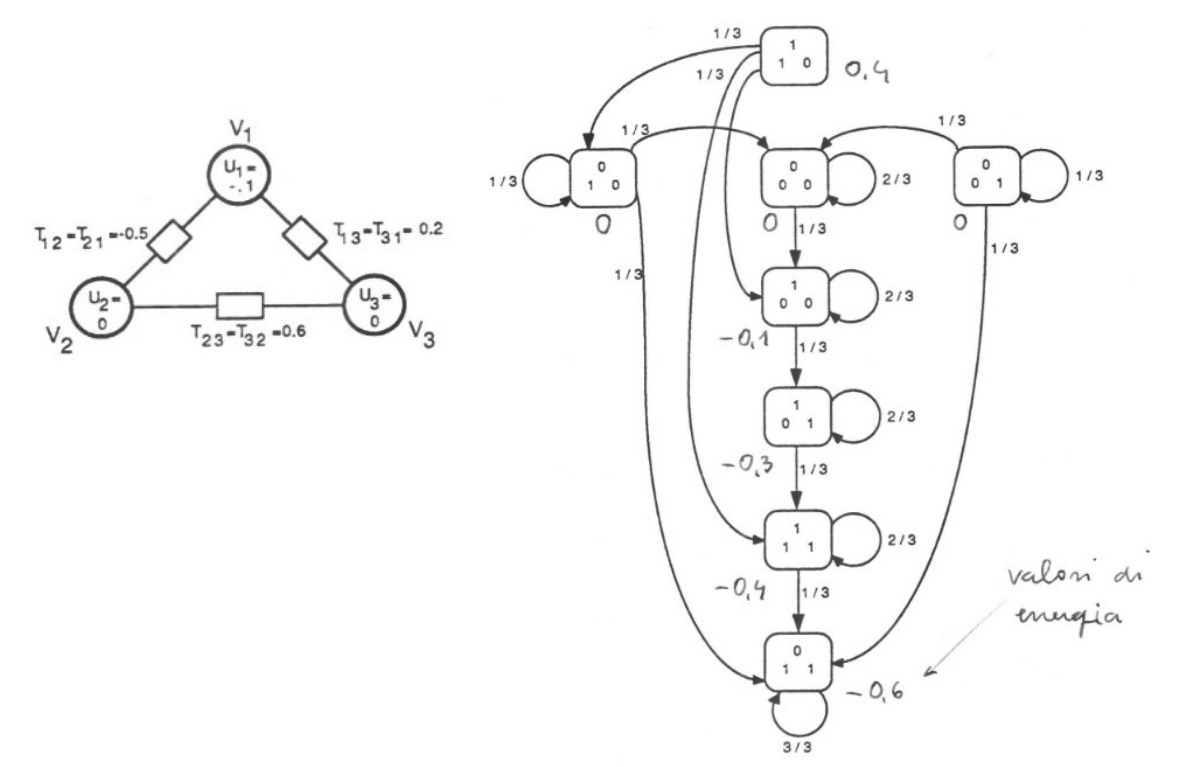
\includegraphics[ width=1.1\linewidth, height=\textheight, keepaspectratio]{./pics/reteHopfieldBase.jpg}
    \caption{Rete di Hopfield costituita da $3$ neuroni, collegati ad anello.
    Ciascun neurone è collegato ad ogni altro mediante una particolare
conduttanza $T_{ij}$, che soddisfa la relazione di simmetria $T_{ij} = T_{ji}$.
Si osserva, sulla destra, l'evoluzione probabilistica della rete, con
decremento dell'energia. Non sono ammessi incrementi energetici.}
    \label{fig:reteHopfieldBase}
\end{figure}

I neuroni possono, almeno secondo una particolare configurazione iniziale, non
presentare un valore dell'uscita adeguato ai valori presenti all'ingresso. In
ogni istante discreto, ciascun neurone ha la medesima probabilità di essere
eccitato (firing), cioè si può verificare la compatibilità del suo valore di
uscita sulla base della somma pesata degli ingressi. Potrebbe darsi che la
somma degli ingressi sia maggiore della soglia $U_i$, ma che il valore d'uscita
sia basso, o viceversa che la somma degli ingressi presenti un valore basso, con uscita alta --- in tal caso, avremo che il neurone \emph{non è soddisfatto}, cioè
è in una condizione di disagio. Esso vorrebbe vedere la propria coerenza
soddisfatta: tanto più i neuroni di una rete di Hopfield sono soddisfatti,
tanto minore sarà l'energia associata allo stato che produrrà tale
soddisfacimento. 

Il modello che Hopfield suggerisce per superare tale
difficoltà è quello di \emph{verificare}, neurone per neurone, la coerenza fra i
valori ai suoi ingressi e il suo valore d'uscita, con una verifica che avviene
in tempo discreto. Qualora non ci fosse coerenza, il neurone andrà modificato,
ottenendo un nuovo stato della rete. In ogni caso, il fenomeno a cui si assiste
è quello per cui ad ogni variazione l'energia della rete cala complessivamente.
Il procedimento di verifica proposto da Hopfield è del tutto aleatorio, e consiste
nell'aggiustamento progressivo dei pesi, calando di volta in volta di energia. Secondo la legge dei grandi numeri, la rete si evolverà percorrendo i vari passi, fino a terminare in una configurazione a minima energia: la configurazione di \emph{minimo locale} dell'energia della rete.
Una volta raggiunta la configurazione di minimo locale dell'energia, non
si può più uscire dalla configurazione. Il minimo dell'energia della rete,
dunque, dovrà corrispondere in qualche maniera alla soluzione cercata. 

Risolvere un problema con una rete di Hopfield, dunque, necessita di un passo
iniziale di \emph{codifica}, cioè che il procedimento di minimazione
dell'energia della rete, cioè la minimazione di una forma quadratica, abbia un
corrispettivo con la soluzione del problema desiderato. In linea di principio,
avendo a disposizione una valida codifica, è possibile risolvere il problema
semplicemente minimizzando l'energia della rete corrispondente, con il
procedimento di verifica in tempi discreti visibile in
Figura~\ref{fig:reteHopfieldBase}.

\subsection{Gli stati stabili}

Specialmente per le macchina a topologia più complessa, possono esistere
configurazioni di minimo locale dell'energia della rete che però non sono
configurazioni di \emph{minimo globale}.

A volte potrebbe risultare comodo imporre la stabilità di uno stato, per
esempio per l'applicazione delle reti al concetto di \emph{memoria
indirizzabile}. Per fare ciò, si impongono delle equazioni alla rete, di modo
da eleggere determinati neuroni della rete come stabili. Un esempio di ciò è
mostrato in Figura~\ref{fig:reteHopfieldWellState}.

\begin{figure}[h]
    \centering
    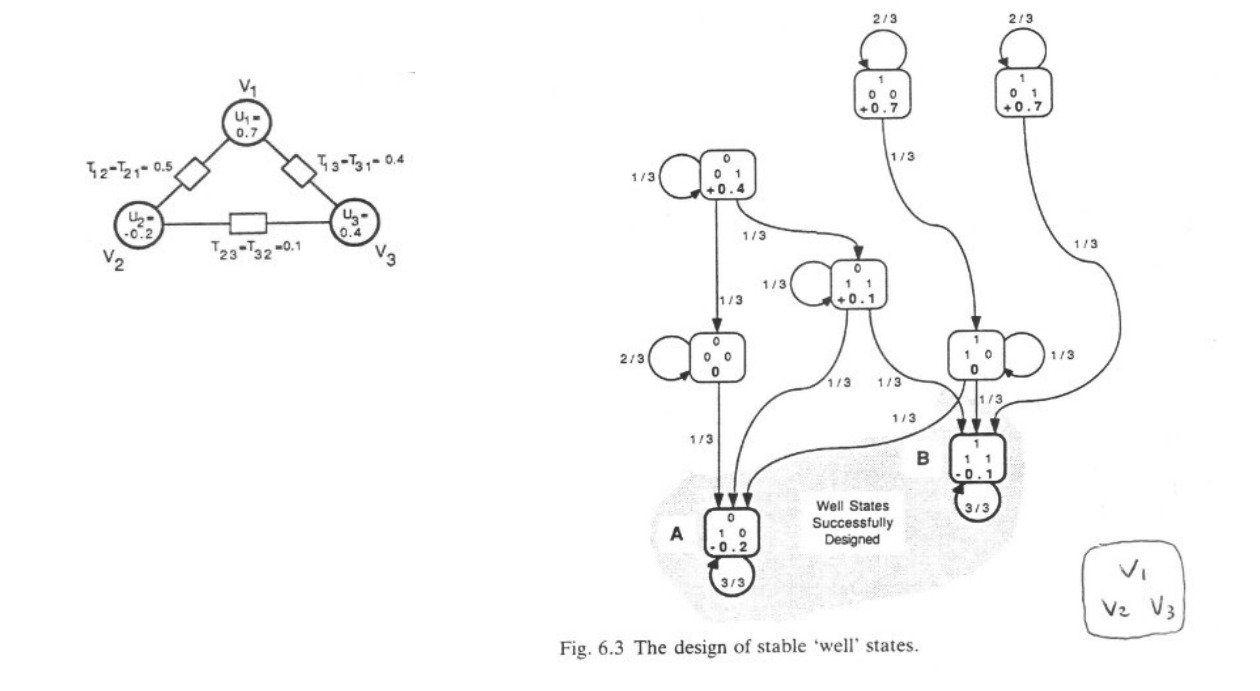
\includegraphics[ width=1.2\linewidth, height=\textheight, keepaspectratio]{./pics/reteHopfieldWellState.jpg}
    \caption{Reti di Hopfield, dove i neuroni al livello di energia più basso
    sono eletti \emph{stati stabili}.}
    \label{fig:reteHopfieldWellState}
\end{figure}



Tipicamente, per reti aventi $n$ neuroni è possibile eleggere $\log (n)$ stati
come stabili, esibendo dunque una crescita di tipo logaritmico.

Se si vuole imporre uno stato stabile, è necessario determinarlo con l'opportuna equazione. Supponiamo di voler imporre lo stato stabile $V_1 = 0$; per fare ciò, bisogna imporre $$T_{12} V_2 + T_{13} V_3 - U_1 < 0,$$ relativo al sistema di equazioni 


$$
\left\{
    \begin{array}{l}
    T_{12} - U_1 < 0 \\
    U_2 < 0 \\
    T_{23} - U_3 < 0
    \end{array}
\right.,
$$

che corrisponde all'imposizione dello stato stabile A in
Figura~\ref{fig:reteHopfieldWellState}. Sempre facendo riferimento alla stessa
rete, imporre lo stato stabile B significherebbe vedere soddisfatto il sistema
di equazioni

$$
\left\{
    \begin{array}{l}
        T_{12} + T_{13} - U_1 < 0 \\
        T_{12} + T_{23} - U_2 > 0 \\
        T_{23} + T_{13} - U_3 > 0 \\
    \end{array}
\right. .
$$

Infatti, avendo definito le quantità nella seguente maniera,

$$
\begin{array}{ll}
    T_{12} = T_{21} = 0,5 & U_1 = +0,7\\
    T_{13} = T_{31} = 0,4 & U_1 = -0,2\\
    T_{23} = T_{32} = 0,1 & U_1 = +0,4
\end{array}
$$

si ha che, per l'equazione di stato A (a sinistra), e l'equazione di stato B (a
destra)

$$
\left\{
    \begin{array}{llllll}
        0,5 - 0,7 < 0 & \leftrightarrow & \mbox{ Sì } & 0,5 + 0,4 - 0,7 > 0 & \leftrightarrow & \mbox{ Sì } \\
        -0,2  < 0 & \leftrightarrow & \mbox{ Sì } & 0,5 + 0,1 + 0,2 > 0 & \leftrightarrow & \mbox{ Sì } \\
        -0,1 - 0,4 < 0 & \leftrightarrow & \mbox{ Sì } & 0,1 + 0,4 - 0,4 > 0 & \leftrightarrow & \mbox{ Sì }
    \end{array}
\right.
$$

ed ambedue gli stati sono, di conseguenza, soddisfatti. In
Figura~\ref{fig:reteHopfieldWellState} essi corrispondono agli stati stabili
$010$ e $111$.

\subsection{La macchina di Boltzmann}

Può capitare che per una data rete di Hopfield vi siano alcuni minimi locali,
detti anche \emph{falsi minimi}; come ad esempio mostrato in
Figura~\ref{fig:retiMinimiLocali}; la soluzione corrispondente al minimo
globale potrebbe quindi non corrispondere a quella trovata mediante
l'evoluzione, se la rete è incappata in un minimo locale. Ciascun minimo locale
è, di fatto, uno stato stabile, dal quale nel caso vi si incappasse, non si
potrebbe uscire, poiché il livello di energia non può mai aumentare. 

Di solito,
si desidera che l'evoluzione converga verso gli stati stabili scelti, oppure
verso un minimo globale --- i minimi locali, tuttavia, risulterebbero essere
alla stregua di ``falsi'' stati stabili, che andrebbero a minare il
comportamento desiderato della rete, per il quale sarebbe desiderabile ottenere
una soluzione unica, e corrispondente al minimo globale (o comunque a stati
stabili dal valore sufficientemente basso di energia). 

\begin{figure}[h]
    \centering
    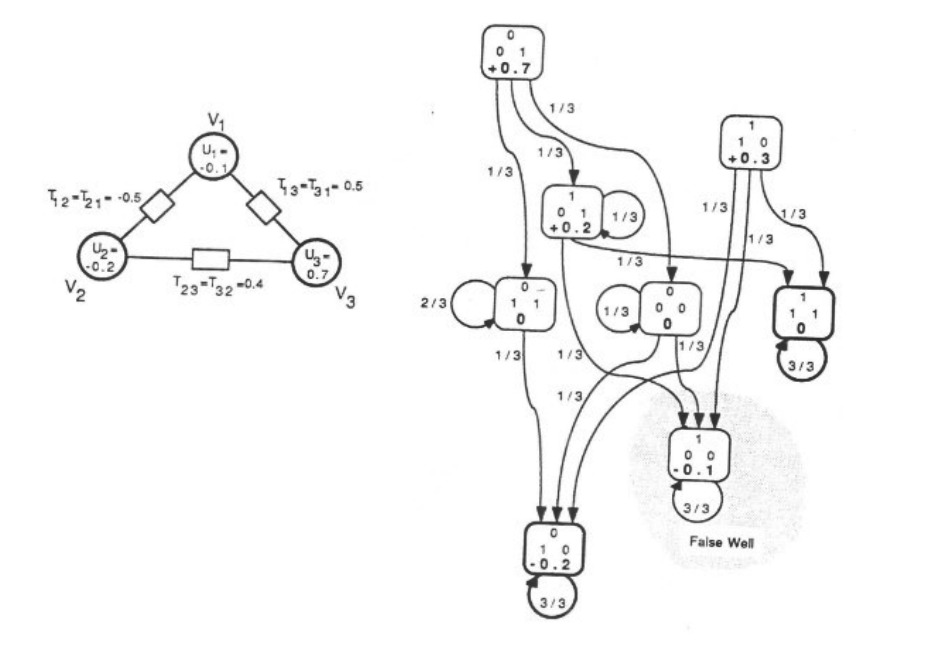
\includegraphics[ width=1.2\linewidth, height=\textheight, keepaspectratio]{./pics/retiMinimiLocali.jpg}
    \caption{Il problema dei \emph{falsi minimi}, anche detti minimi locali.}
    \label{fig:retiMinimiLocali}
\end{figure}



Con un po' di fortuna, i minimi locali possono avere un valore prossimo al
minimo assoluto; tuttavia ciò non è per nulla garantito, e non esistono criteri
matematici per stabilire la qualità della soluzione ottenuta. In altre parole,
\emph{non possiamo sapere a priori se la qualità della soluzione ottenuta},
incappando in uno stato stabile artificiale o di minimo locale, \emph{è
sufficientemente buona oppure non lo è.} 

Ciò rappresenta in ultima analisi un evidente difetto delle reti neurali di
Hopfield, poiché diversamente al paradigma della computazione procedurale dove
è sempre e comunque possibile ricondursi in qualche maniera al modello di
Turing o al modello RAM, e dunque ai teoremi studiati in tale ambito, nel
paradigma di computazione delle reti di Hopfield non c'è alcun criterio
matematico in grado di stabilire \textbf{a priori} la qualità di una
determinata soluzione.

Una soluzione al problema dei minimi locali imprevisti arrivò a cavallo degli
anni $80$, quando si cercò di superare il problema evocando la cosiddetta
\textbf{Boltzmann machine}, un modello della rete di Hopfield dove uno stato può
vedere \emph{aumentata la propria energia secondo una legge probabilistica},
violando dunque l'assunzione di base tale per cui l'energia complessiva della
rete può soltanto diminuire. Ciò viene attuato riscaldando in maniera
\emph{probabilistica} la rete, introducendo cioè una funzione \emph{sigmoidale}
dipendente da un parametro $T$, detto \emph{temperatura del neurone}; le
funzioni sigmoidali della macchina di Boltzmann sono progettate in modo tale
che una temperatura più elevata corrisponda a sigmoidi meno rigide, e
temperature che tendono allo $0$ termico corrispondono a sigmoidi molto simili
al tradizionale gradino.

Dunque, con il modello della macchina di Boltzmann,
temperature della rete molto basse e prossime allo zero termico produrrebbero
un comportamento della rete di Hopfield del tutto simile a quanto incontrato
sino ad ora, cioè ad un'evoluzione nella quale non sono ammessi aumenti del
livello dell'energia --- viceversa, ad alte temperature del neurone si
assiste mano a mano a potenziali fenomeni in cui, al passaggio successivo, la
rete si è evoluta verso uno stato avente una maggiore energia rispetto a quello
precedente. L'idea di base della macchina di Boltzmann è quella di poter
``sfuggire'' all'attrazione dovuta ai minimi locali, introducendo la
possibilità probabilistica di poter ``tornare indietro'' e tentare una strada
evolutiva differente. La probabilità con cui un determinato stato possa
sfuggire dal minimo locale in cui risiede dipende dalla temperatura $T$ --- più
essa è alta, maggiore sarà la probabilità per lo stato di aumentare la propria
energia e percorrere un'evoluzione differente.

\begin{figure}[h]
    \centering
    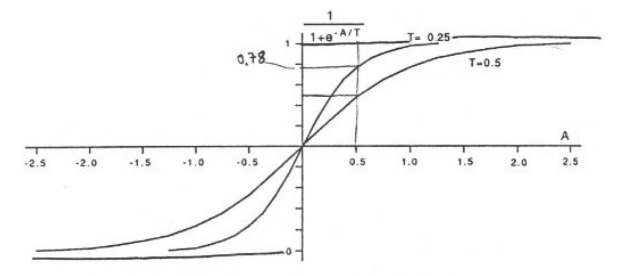
\includegraphics[ width=1.0\linewidth, height=\textheight, keepaspectratio]{./pics/boltzmannMachine.jpg}
    \caption{La funzione di attivazione probabilistica, con la sua tipica forma
    ``ad esse'' e comportamento dipendente dalla temperatura $T$. La sua forma
sarà tanto più simile al gradino ideale quanto la sua temperatura sarà tendente
allo $0$.}
    \label{fig:boltzmannMachine}
\end{figure}



Supponendo di disporre di un valore di attivazione $A = \sum_{j\neq i} T_{ij}
V_j - U_i$ pari a $ A = +0.5$, e una temperatura di $T=0,25$, avremo che la
probabilità di eccitazione del neurone sarà pari a $0,78$ invece che pari ad
$1$, come espresso in Figura~\ref{fig:boltzmannMachine}. Dunque, si dà la
possibilità al neurone di \emph{risalire la china dell'energia}, violando il
comportamento originale che invece aveva nella rete di Hopfield --- con questo
stratagemma, la rete può probabilisticamente ``scappare'' dagli stati di minimo
locali non desiderati. Si aggiungono dunque nuovi percorsi che con una certa
probabilità dipendente dalla temperatura $T$ \emph{aumentano l'energia
della rete}: valori più alti di temperatura garantiscono una maggiore
probabilità di aumento dell'energia. 

Questo procedimento è chiamato \textbf{simulated annealing}, termine tratto
dalla metallurgia (ricottura), dove variazioni di temperatura di un materiale
sono adoperate per ottenere determinate caratteristiche dal materiale in
questione. In particolare, la rete di Hopfield sarà inizialmente molto calda,
per poi raffreddarsi progressivamente. La Figura~\ref{fig:retiBoltzmannMachine}
illustra un esempio di rete dove esiste una possibilità di ``risalire la
china'', o più precisamente c'è una probabilità non nulla di ritornare ad un
livello di energia superiore.

\begin{figure}[h]
    \centering
    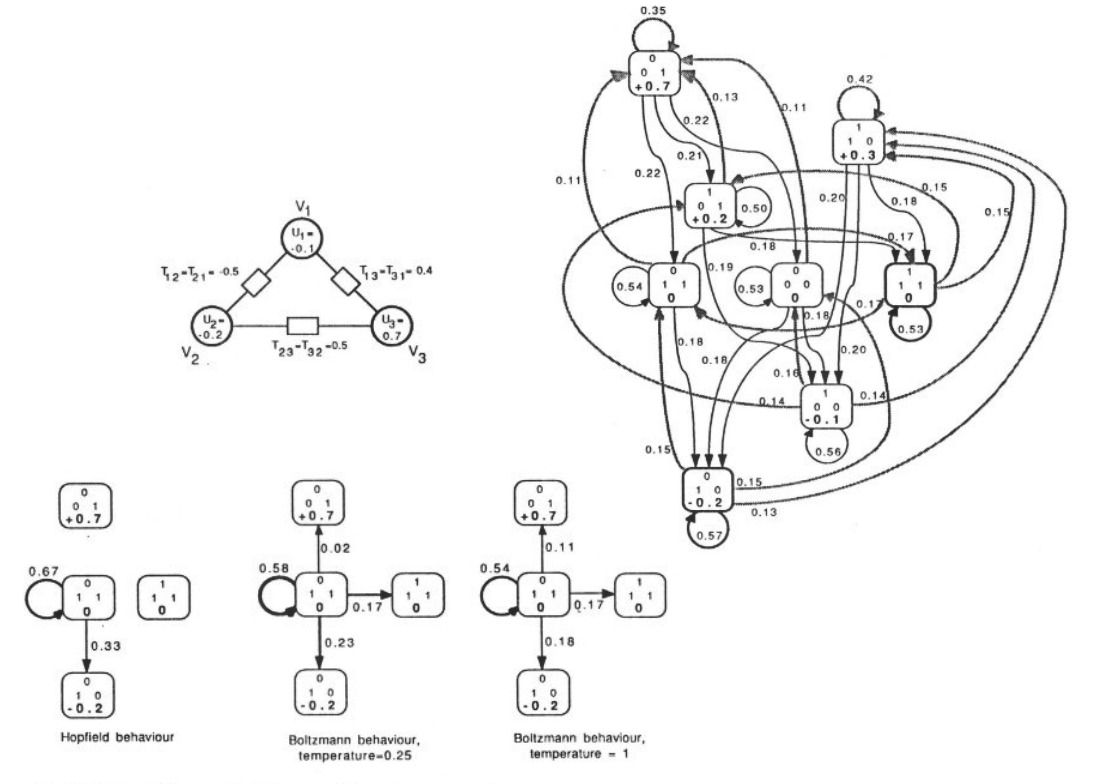
\includegraphics[ width=1.3\linewidth, height=\textheight, keepaspectratio]{./pics/retiBoltzmannMachine.jpg}
    \caption{Probabilità di transizione a differenti temperature $T$ (in
    basso); rete di Hopfield con estensione a macchina di Bolztmann (sopra).}
    \label{fig:retiBoltzmannMachine}
\end{figure}


E dunque grazie allo stratagemma della macchina di Boltzmann è possibile
progettare una rete di Hopfield che sia quantomeno robusta al problema dei
minimi locali, introducendo di fatto una sorta di \emph{perturbazione} alla
funzione di attivazione, che rende concretamente e probabilisticamente
possibile percorrere strade nuove e che consentono alla rete di ``fuoriuscire''
dalla situazione di stallo causata dallo stato di minimo locale in cui si
troverebbe imprigionata.


\section{La rete continua di Hopfield}

\begin{figure}[h]
    \centering
    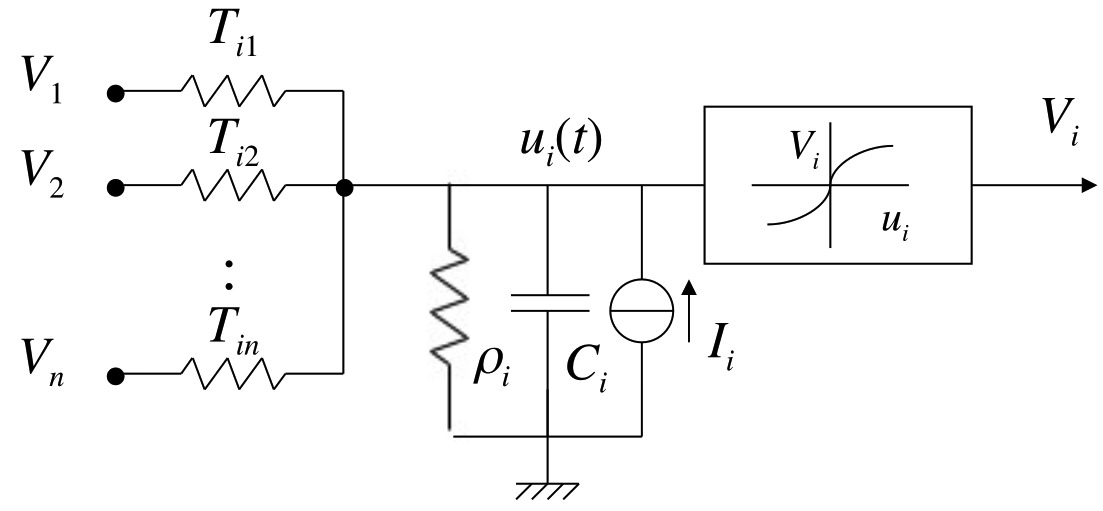
\includegraphics[ width=1.0\linewidth, height=\textheight, keepaspectratio]{./pics/reteHopfieldContinua.jpg}
    \caption{La \emph{rete continua di Hopfield}.}
    \label{fig:reteHopfieldContinua}
\end{figure}

La \textbf{rete continua di Hopfield} rappresenta un cambio di paradigma: mentre
prima la verifica sullo stato veniva fatto in tempi discreti, assumendo una
certa probabilità di interrogazione di un neurone, nella rete continua ogni
neurone è, con continuità, connesso ad ogni altro neurone e la verifica della
loro coerenza avviene istante per istante, mediante un \emph{circuito
analogico}, con un amplificatore operazionale posto a produrre la funzione di
attivazione.

L'idea quindi è quella di lasciar evolvere il sistema composto dalla rete
neurale, facendo sì che le grandezze elettriche in questione sviluppino il loro
transitorio completamente: il risultato finale sarà la rete a minor energia.

Il valore d'uscita dipende da una funzione sigmoidale, ad esempio
$$V_i = g_i(u_i(t)) = \tanh (\frac{u_i(t)}{u_0}).$$ Alle conduttanze
d'ingresso, viene aggiunto un gruppo circuitale
resistenza-condensatore-generatore di corrente che produce correnti
parallelamente a quelle di ingresso, cioè che si somma a quelle di ingresso.
La totale conduttanza di neurone sarà pari a

$$ \frac{1}{R_i} = \frac{1}{\rho_i} + \sum_j \frac{1}{R_j}, $$

e tramite le leggi di Norton, si ottiene l'equazione al nodo d'ingresso del
neurone,

\begin{equation}\nonumber
    \sum_j (V_j - u_j(t)) T_{ij} + I_i = C_i \frac{du_i(t)}{dt} + \frac{u_i(t)}{\rho_i}
\end{equation}

mentre l'energia della rete sarà


\begin{equation}
    E = -\frac 1 2 \sum_{ij, j\neq i} T_{ij} V_i V_j + \sum_i \frac{1}{R_i}
    \int_0^{V_i} g_i^{-1} (V) dV - \sum_i I_i V_i.
\end{equation}

Calcolando la variazione dell'energia, 

$$ \frac{dE}{dt} = \sum_i \frac{dE}{dV_i} \frac{dV_i}{dt},$$ pertanto si avrà che

\begin{eqnarray}\nonumber
    \frac{dE}{dV_i} & = & -\sum_j T_{ij}V_j + \frac{u_i}{R_i} - I_i = -C_i\frac{du_i}{dt} \\\nonumber
    \frac{dE}{dt}   & = & -\sum_i \left(\sum_j T_{ij}V_j + \frac{u_i}{R_i} - I_i\right)\frac{dV_i}{dt} = -\sum_i C_i\frac{du_i}{dt}\frac{dV_i}{dt} \\\nonumber
                    & = & -\sum_i C_i(\frac{du_i}{dV_i})\left(\frac{dV_i}{dt}\right)^2 \\\nonumber
                    & = & -\sum_i g_i^{-1}(V_i)C_i\left(\frac{dV_i}{dt}\right)^2 \leq 0,
\end{eqnarray}

dove si è osservato che $g_i^{-1}(V_i) > 0, \forall V_i$ poiché monotona
crescente. In definitiva la variazione netta di energia della rete sarà

\begin{equation}
    \frac{dE}{dt} \leq 0,
\end{equation}

con l'uguaglianza a zero rispettata solo ed esclusivamente nel caso in cui
$\displaystyle \frac{dV_i}{dt} = 0, \forall i$. Dunque, anche nel caso della
rete continua di Hopfield la variazione di energia sarà sempre negativa.

In ultima analisi, \emph{il tempo di risposta} di una rete di Hopfield dipende
esclusivamente dalla costante di tempo $\tau = C_i R_i$ del neurone, poiché per ottenere
una soluzione è necessario che il transitorio dell'evoluzione della rete abbia
termine. Di fatto, il tempo di risposta non dipende dalla complessità della
rete, bensì unicamente dalla costante di tempo --- diversamente per quanto
accadeva con le reti discrete di Hopfield.

Degno di nota è il fatto che il rapporto ingresso-uscita è fissato da una
sigmoide, non è garantito che il valore d'uscita sia ad un valore nettamente
basso o nettamente alto, cioè non è garantito un perfetto comportamento a
soglia. Esistono infatti valori in concomitanza con lo $0$ d'ingresso che
possono suscitare dubbi interpretativi, cioè il neurone potrebbe collocarsi ad
un valore intermedio fra valore alto e basso. 


\section{Soluzione dei problemi con la rete di Hopfield}

Con una rete di Hopfield si può risolvere un problema solo se esso può essere
codificato nei termini della \emph{minimazione di una forma quadratica}. La
soluzione sarà \emph{ottima} se l'energia ottenuta è quella corrispondente al
minimo assoluto --- viceversa, sarà \emph{sub-ottimale} se l'energia ottenuta
corrisponderà invece a quella di un minimo locale, o comunque di uno stato
stabile vero o falso che sia ad energia maggiore di quella fornita dal minimo
globale.

La strategia è la seguente: individuata la forma quadratica associata al
problema, per confronto si ricavano i valori $T_{ij}$ ed $I_i$ che consentono
la costruzione della rete. Successivamente, la rete è lasciata evolvere; la
soluzione corrispondente viene prelevata e il problema viene risolto con la
soluzione ricavata mediante la codifica.

\subsection{Il problema della memoria indirizzabile}

Si desidera che $V^s(s=1,2,\dots, n)$ siano stati stabili in una rete dotata di
$n$ neuroni. 

La quantità da minimizzare sarà $\hat E = -\frac 1 2 \sum_s (V^s\cdot
V)^2$, con $V=V^s$ valore negativo di energia minimo: ciò accade poiché siamo
di fronte ad un prodotto scalare che massimizza la quantità all'interno della
sommatoria, con il risultato di minimizzare il valore dell'energia. 

Se $V$ è
casuale e $(-1 \leq V_i \leq +1)$, la $\hat E$ risulterà essere circa nulla --
eseguendo un prodotto scalare fra due vettori sostanzialmente molto differenti;
il valore minimo si raggiunge con $V=V^s$, ed è tale che $\hat E = -\frac 1 2
n^2$. 

Bisogna in pratica fissare anticipatamente i $V^s$ di stato stabile, e
con essi si imposta l'equazione $$ E = -\frac 1 2 \sum_s (V^s V)^2 = \dots =
-\frac 1 2 \sum_i \sum_j (\sum_s V_i^s V_j^s)V_i V_j,$$ ma sappiamo anche che

$$E= -\frac 1 2 \sum_{ij} T_{ij}V_i V_j - \sum_i I_i V_i.$$ Dal confronto fra
le due equazioni è presto ricavato che 

$$
\left\{
    \begin{array}{lll}
        T_{ij} & = & \sum_s V_i^s V_j^s \\
        I_i & = & 0
    \end{array}
\right.
$$

cioè abbiamo trovato la conduttanze e il valore del generatore ideale di
corrente per poter costruire la rete continua di Hopfield associata al
problema impostato come minimazione di un funzionale quadratico. Innescata la
rete, essa andrà presumibilmente (a meno di falsi stati stabili) a stabilirsi
in uno degli stati $V^s$ determinati dal progettista.

\subsection{Il problema delle somme parziali}\label{sec:sommeParziali}

Il problema delle somme parziali è sostanzialmente intrattabile. Vi sono alcuni
interi $a = a_1, a_2, \dots, a_n$ e alcuni numeri binari $ V = V_1, V_2, \dots,
V_s, V_i \in \{0,1\}$, con $S$ risultato del prodotto scalare fra $a$ e $V$ e
si chiede di trovare il vettore $V$ sapendo che

$$a \cdot V = S$$ e conoscendo $a$ ed $S$. In altre parole, si chiede di
invertire il prodotto scalare trovando il vettore di binari $V$ tale da fornire
il risultato $S$ a fronte del prodotto con il vettore $a$ di numeri interi,
anch'esso noto a priori.

Il funzionale quadratico da minimizzare sarà il seguente,

\begin{equation}
    E = \frac 1 2 (S - \sum_i a_i V_i)^2 - \frac 1 2 \sum_i a_i^2 V_i(V_i - 1),
\end{equation}

dove il secondo termine rappresenta le condizioni al contorno tali per cui esso
è nullo esclusivamente nel caso in cui $V_i \in \{0,1\}$, ovvero esso funge da
\emph{penalità} per tutti i termini tali che $V_i \neq 0$ oppure $V_i \neq 1$,
in quanto termine positivo da sommarsi.

Dunque,

\begin{eqnarray}\nonumber
    E & = & \frac 1 2 (S - \sum_i a_i V_i)^2 - \frac 1 2 \sum_i a_i^2 V_i(V_i - 1) \\\nonumber
      & = & -\frac 1 2 \sum_i \sum_{j \neq i} (-a_i a_j) V_i V_j - \sum_i(-\frac{a_i^2}{2} + Sa_i)V_i + \frac{S^2}{2},
\end{eqnarray}

e dunque si avrà

$$T_{ij} = \sum_{j\neq i} (-a_i a_j),$$
$$I_i = \sum_i (-\frac{a_i^2}{2} + Sa_i).$$

\begin{figure}[h]
    \centering
    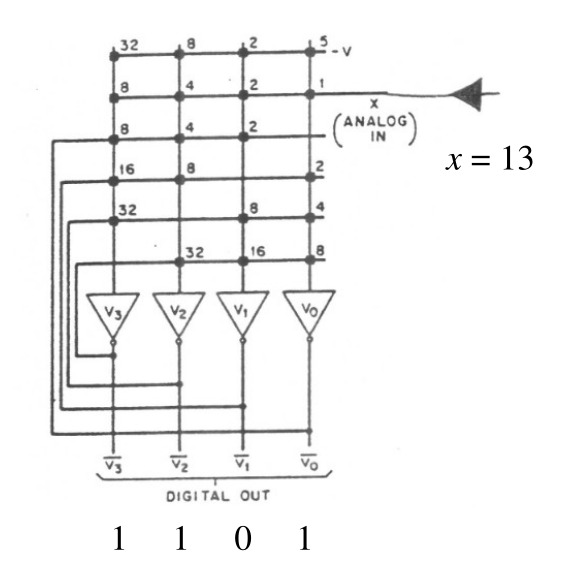
\includegraphics[ width=1.0\linewidth, height=\textheight, keepaspectratio]{./pics/convertitoreAD.jpg}
    \caption{Un dispositivo convertitore Analogico-Digitale. Esso può essere
    modellato mediante una rete continua di Hopfield.}
    \label{fig:convertitoreAD}
\end{figure}



Supponendo di avere $a_i = 2^i$ la soluzione si risolve in tempo polinomiale,
ed ha un \emph{unico minimo assoluto}. Vi è una forte dipendenza fra la natura
del problema e la quantità di minimi locali --- se la complessità del problema
è elevata, la risoluzione con la rete di Hopfield diventa maggiormente
difficile a fronte di un più grande numero di minimi locali. La difficoltà del
problema viene pertanto in qualche modo incastonata nella \emph{complessità
strutturale} della rete e dunque in ultima analisi la \textbf{dimensione della
rete dipende dalla complessità del problema}. 

Se si intende risolvere il
problema delle somme parziali con $n=1000$, la rete prodotta sarà di enormi
dimensioni e complessità, con ciascun coefficiente $T_{ij}$ e generatore ideale
di corrente $I_i$ da determinare di conseguenza. Diversamente dal caso del
paradigma a computazione procedurale, dove la complessità è di tipo
\emph{temporale}, nel paradigma a reti neurali l'aspetto temporale è invece di
secondaria rilevanza, poiché è sempre possibile scegliere un valore di capacità
sufficientemente piccolo (ad esempio, dell'ordine dei pico-Farad\footnote{Si
ricorda a tal proposito che $\tau = C_i R_i$ con $R_i$ totale resistenza di
ingresso del neurone.}) ed ottenere una risposta della rete pressoché
istantanea. La complessità delle reti neurali, però, si sviluppa lungo la
dimensione della loro \emph{struttura}.

\subsection{Il traveling salesman problem}

Il traveling salesman problem è un problema presumibilmente intrattabile --
benché esistano ottimi algoritmi euristici di tipo approssimato, la migliore
soluzione esatta viene ricoperta in tempo almeno esponenziale.

Supponendo di trovarci di fronte $n$ città A, B, C, \dots, e di possedere le
distanze reciproche $d_{AB}, d_{AC}, d_{BC}, \dots$, e così via. La tecnica
adoperata per la codifica della soluzione è quella di una \emph{matrice
città----percorso ottimale}, ad esempio

\begin{table}[ht]
\centering
\begin{tabular}{c|ccccc}
    & 1 & 2 & 3 & 4 & 5 \\
    \hline
A   & 0 & 1 & 0 & 0 & 0 \\
B   & 0 & 0 & 0 & 1 & 0 \\
C   & 1 & 0 & 0 & 0 & 0 \\
D   & 0 & 0 & 0 & 0 & 1 \\
E   & 0 & 0 & 1 & 0 & 0
\end{tabular}
\end{table}
\bigskip

è la matrice che corrisponde alla codifica del percorso C-A-E-B-D.


Dunque, esprimendo il funzionale dell'energia da minimizzare, si ottiene


\begin{eqnarray}\nonumber
    E & = & \frac \alpha 2 \sum _x \sum_i \sum_{j \neq i} V_{X_i}V_{X_j} +
    \frac \beta 2 \sum_i \sum_X \sum_{X \neq Y} V_{X_i}V_{Y_i} \\\nonumber
      & + & \frac \delta 2 (\sum_x \sum_i V_X - n)^2 + \frac \gamma 2 \sum_X
      \sum_{X \neq Y} \sum_i d_{XY} V_{X_i}(V_{Y_{i + 1}} + V_{Y_{i - 1}}).
\end{eqnarray}

Si tratta di un funzionale particolarmente complesso, composto da $4$ distinti termini:
\begin{enumerate}
    \item il primo termine è la condizione al contorno per le righe, pari a
        zero se ogni riga contiene esclusivamente un singolo $1$;
    \item il secondo termine è la condizione al contorno per le colonne, pari a
        zero se ogni colonna contiene esclusivamente un singolo $1$;
    \item il terzo termine conta il numero di $1$: esso è pari a zero solo se
        vi sono \emph{esattamente} $n$ termini $1$ nella matrice;
    \item il quarto ed ultimo termine, infine, è quello necessario per
        minimizzare il funzionale relativo al percorso.
\end{enumerate}

\begin{figure}[h]
    \centering
    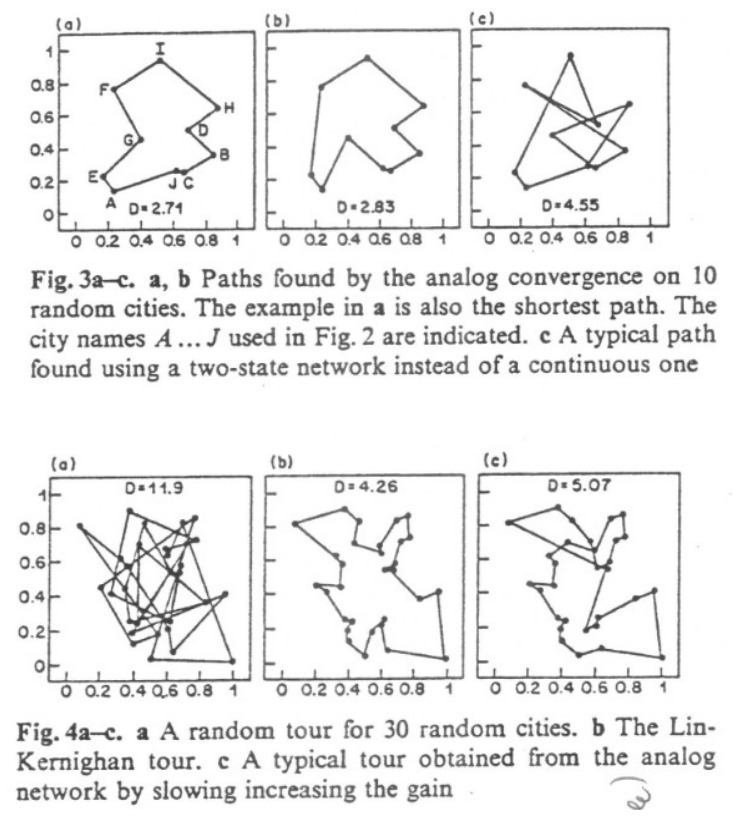
\includegraphics[ width=1.0\linewidth, height=\textheight, keepaspectratio]{./pics/retiTSPEsempi.jpg}
    \caption{Esempi della risoluzione del travelling salesman problem con reti
    neurali di Hopfield.}
    \label{fig:retiTSPEsempi}
\end{figure}






\section{Sommario delle caratteristiche delle reti neurali}

\begin{quote}
    A.K. Dewdney 1997, 

        \emph{``Although neural nets do
solve a few toy problems, their powers of computation
are so limited that I am surprised anyone takes them
seriously as a general problem-solving tool.''}
\end{quote}
\bigskip

I pregi delle reti neurali di Hopfield sono di seguito elencati,

\begin{itemize}
    \item esse rappresentano un ``nuovo'' ed interessante \emph{paradigma
        computazionale};
    \item sono \emph{robuste rispetto ai guasti} dei singoli neuroni;
    \item le risposte sono \emph{in tempo reale}, nel caso di realizzazione ``fisica''
        con hardware;
    \item forniscono un'interessante \emph{metafora biologica}.
\end{itemize}

I difetti invece rendono molto difficile il loro utilizzo. In particolare,
\begin{itemize}
    \item manca una adeguata \emph{formalizzazione matematica};
    \item non vi sono \emph{garanzie sulla qualità} della soluzione trovata,
        non si ottengono in genere soluzioni ottime;
    \item soffrono del \emph{problema dei falsi minimi};
    \item sono inferiori ad \emph{algoritmi dedicati};
    \item necessitano di un'\emph{altissima complessità strutturale} che
        dipende dall'istanza del problema;
    \item \emph{dipendono fortemente dai pesi del problema}: cambiando
        \textbf{istanza} del problema, cambiano \textbf{tutti i coefficienti},
        rendendo di fatto \textbf{praticamente irrealizzabili} queste reti se
        dotate di una complessità apprezzabile.
\end{itemize}


\chapter{La computazione DNA}

La \textbf{computazione DNA} è un metodo di computazione che corrisponde ad una
procedura di \emph{ricerca esauriente}: tutte le possibili soluzioni vengono
costruite in modo sistematico, e vengono poi analizzate ``in vitro'', cioè una
per volta, per poi conservare esclusivamente le soluzioni desiderate. Non si
tratta, perciò, di una nuova tecnica con differenze dal punto di vista
strutturale, bensì di un metodo molto efficace per realizzare una ricerca
esauriente della soluzione.

Il modello a computazione DNA adotta il DNA biologico come contenitore delle
informazioni: le sue dimensioni sono talmente ridotte da permettere una ricerca
esauriente in spazi ridottissimi. Nella pratica, si fanno uso di tantissimi DNA
per l'individuazione di soluzioni desiderate. La risultante ricerca esauriente
non viene adottata mediante un classico algoritmo, bensì in modo ``nativo''
tramite l'uso dei DNA.

Storicamente, le scienze matematiche e quelle naturali si sono evolute seguendo
due rami ben distinti. Attorno agli anni 50, la biologia molecolare scoprì il
DNA --- immediatamente furono aperte nuove strade, compresa quella
dell'\emph{informatica nella biologia}. In particolare, furono usati risultati
dell'\emph{algoritmica} per trattare le lunghissime sequenze del DNA e il
ripiegamento delle proteine e t-RNA, ambedue problemi più facilmente trattabili
con le nozioni avanzate dell'informatica teorica e più precisamente
dell'algoritmica. Non molto tardi, le \emph{misure dell'informazione} figlie
della teoria dell'informazione furono adottate anche per la costruzione degli
\emph{alberi filogenetici}, diagrammi che mostrano le relazioni fondamentali di
discendenza comune di gruppi tassonomici di organismi. 

Più tardivamente, ovvero attorno alla metà degli anni 90, furono aperte strade
nella direzione opposta: il sequenziamento del DNA fu di ispirazione per il
nuovo modello di computazione appunto ``a DNA'' (Adleman, 1994). Allora fu
sottolineata la capacità di manipolare le stringhe astratte dell'informatica
tramite una \emph{codifica nel DNA} --- senza occuparsi del significato della
struttura chimica, fisica, biofisica e genetica propriamente attribuiti alle
molecole del DNA. Implicitamente si intende adoperare il DNA per contenere
informazioni tramite i simboli (codificati) nel DNA, piuttosto che per scopi
``biologici'' e legati a quanto si faceva in passato.

L'idea è quella di risolvere con una computazione DNA certi problemi che sono
\emph{strutturalmente difficili}, per i quali algoritmi efficienti non sono
noti. Esempi di tali problemi sono il \emph{problema delle somme parziali}, il
\emph{problema della fattorizzazione di un intero}, e la determinazione del
\emph{cammino Hamiltoniano su un grafo}.

I DNA sono basati su lunghissime sequenze di lettere di un \emph{alfabeto
finito}, avente 4 simboli (A, C, G, T), detti \emph{nucleotidi}. Anche le
proteine sono basate su catene molecolari, in particolare su un alfabeto
anch'esso finito di 20 simboli, detti \emph{amminoacidi}. La codifica di queste
catene di simboli può essere effettuata, come è ragionevole aspettarsi,
mediante tecniche informatiche.

Ad esempio, di seguito sono riportate i 20 amminoacidi

\begin{quote}
    \footnotesize{
Alanina (Ala, A)

Acido glutammico (Glu, E)

Arginina (Arg, R)

Glutammina (Gln, Q)

Asparagina (Asn, N)

Istidina (His, H)

Acido aspartico (Asp, D) 

Isoleucina (Ile, I)

Cisteina (Cys, C)

Leucina (Leu, L)

Metionina (Met, M)

Fenilalanina (Phe, F)

Prolina (Pro, P)

Serina (Ser, S)

Treonina (Thr, T)

Tirosina (Tyr, Y)

Valina (Val, V)

Triptofano (Trp, W)

Lisina (Lys, K)

Glicina (Gly, G)
}
\end{quote}

il cui alfabeto può essere opportunamente codificato. Con l'adeguata codifica,
esse sono perciò in grado di \emph{immagazzinare informazioni}.

La computazione DNA è tipicamente adoperata per la soluzione di problemi
\emph{presumibilmente} o \emph{sostanzialmente intrattabili} --- problemi di
difficile soluzione, di cui non sono noti ad oggi algoritmi efficienti.

Dato il \textbf{problema delle somme parziali} descritto in
Sezione~\ref{sec:sommeParziali}, è noto che non è facile trovare gli elementi
costituenti la somma parziale.

Un altro problema di difficile soluzione è quello della \textbf{fattorizzazione
di un intero}: dati $p$ e $q$ interi primi, molto grandi, è facile calcolare
$$n = p \cdot q,$$ mentre è estremamente difficile calcolare $p$ e $q$ a
partire dal solo $n$.

Un ultimo problema, che verrà analizzato di seguito, è il \textbf{problema del
cammino Hamiltoniano su un grafo}, risolto con la computazione DNA proprio da
Adleman nel 1994.

\section{Uso dell'informatica per la risoluzione di problemi di Biologia molecolare}

Leggere il DNA tutto di seguito è tecnologicamente impossibile --- ciò che si
può fare è leggere sequenze di qualche centinaio di basi. Diventa dunque di
estrema rilevanza il problema dell'\textbf{assemblaggio dei
frammenti di DNA}.

Supponendo di voler sequenziare il frammento di DNA 

\begin{center}
\texttt{AGTATTGGCAATCGATGCAAACCTTTTGGCAATCACT}
\end{center}

Si possono adoperare i
cosiddetti \emph{enzimi di restrizione} per estrarre alcune sequenze.
Tipicamente, si estraggono varie sequenze che vanno riordinate, e ritagliate
nel caso vi siano delle sovrapposizioni. Ricostruire la sequenza esatta del DNA
a partire dai lembi di poche centinaia di basi è molto difficile: in un vero
esperimento biologico si hanno lunghezze di DNA da $30000$ a $100000$ basi, con
lunghezze di frammenti che crescono fino a $700$ basi; il numero di frammenti
totale sarà all'incirca dell'ordine di qualche migliaio. 

La strategia che si adopera è quella dell'\emph{allineamento risolutivo}, cioè
quella di andare ad allineare i frammenti a seconda delle loro somiglianze
(string matching). Ad esempio, la seguente sequenza di frammenti è stata
riordinata per allineamento risolutivo, con le corrispondenze che si
manifestano in verticale.

\begin{center}
\texttt{
AGTATTGGCAATC--------CCTTTTGG--------
---------AATCGATG--------TTGGCAATCACT
--------------ATGCAAACCT-------------
AGTATTGGCAATCGATGCAAACCTTTTGGCAATCACT
}
\end{center}


Il secondo problema è quello della \textbf{ricerca di moduli funzionali del DNA},
dove è richiesto di trovare i moduli funzionali del gene avendo sequenze di DNA
relative allo stesso gene, però di organismi differenti. Un modulo funzionale è una
porzione del DNA che svolge un qualche ruolo nella dinamica biochimica della
cellula. Non tutto il DNA viene effettivamente adoperato per i principi
metabolici --- tipicamente, molte parti del DNA sono \emph{ridondanti}.
Attraverso i moduli funzionanti si svolgono le dinamiche interessanti del
funzionamento della cellula. Un esempio di ciò sono \textbf{i geni} --- di
lunghezza molto più corta del DNA, grazie ad essi sono realizzate le proteine
per cui si ha il funzionamento dell'organismo biologico.

I moduli funzionali nel corso delle generazioni possono subire piccole
variazioni nella loro struttura, sia per via dell'evoluzione che per raggi
cosmici o altre radiazioni ionizzanti, presentando lacune o lettere differenti.
Ad esempio, alcune differenze sono presenti nelle catene e frammenti di seguito:

\begin{center}
\texttt{
----------------------AG--TTGTCAATCTTGGCAATCACT
ATCGATTCCGGCCCTTTTGG--AGTATTGGCAATCATGCAAACCT--
---GTCGATCGAATGCAAACCTAGTAATGGCAATCCTATGCTCGATC
-----------------GTACCAGTATTGGCA-TCTGC---------
----------ATCTTCAATTATAGTATTGACAATCTCGCTAGTCG--
---CCGGCTCTAAAATTTGGGGAGTGTTGGCAATCATTCCGGCTCTA
------------ATTGCATGCAAG-ATTGGCAATCATCGA-------
----CGTCGATCCAATTTCAGCAGTAT--GCAATCATTCGTCGATCG}
\end{center}

Pur essendo i moduli di cui sopra formalmente diversi, essi manifestano un
patrimonio comune, presentando una grossa quota di nucleotidi simili dal punto
di vista della \emph{Levenshtein distance} (distanza fra stringhe simile alla
distanza di Hamming fra numeri binari). Dunque, dall'esempio sopra si individua
il modulo funzionale \texttt{AGTATTGGCAATC}.

Per i problemi di cui sopra, la struttura dati importante è quella dello
\textbf{suffix tree} (albero a suffisso). Viene assegnata una stringa, e viene
chiesto di trovare la più lunga sottostringa ripetuta. Un suffix tree può
essere costruito in tempo lineare, rendendo possibile l'individuazione delle
sottostringhe da ricercare appunto in tempo lineare.

Si parte da sinistra, ricopiando l'intera stringa. Ogni stringa dell'albero
viene etichettata con la posizione sulla stringa dalla quale la lettera è stata
determinata (con il \emph{suffisso}), e ad ogni nuova lettera si apre un nuovo
ramo. Ogni qualvolta si ripresenta una medesima lettera, il percorso viene
riutilizzato: si aprirà un ramo solo nel punto dove i due cammini in comune
presentano la prima differenza, ed il nuovo ramo è etichettato a sua volta con
il suffisso indicante la posizione del nodo sulla stringa.

L'interrogazione dell'albero avviene individuando il \emph{nodo a profondità
massima} dell'albero, poiché fino a quel nodo la stringa si è conservata la
stringa la stringa a lunghezza massima su almeno due percorsi.

\begin{figure}[ht]
    \centering
    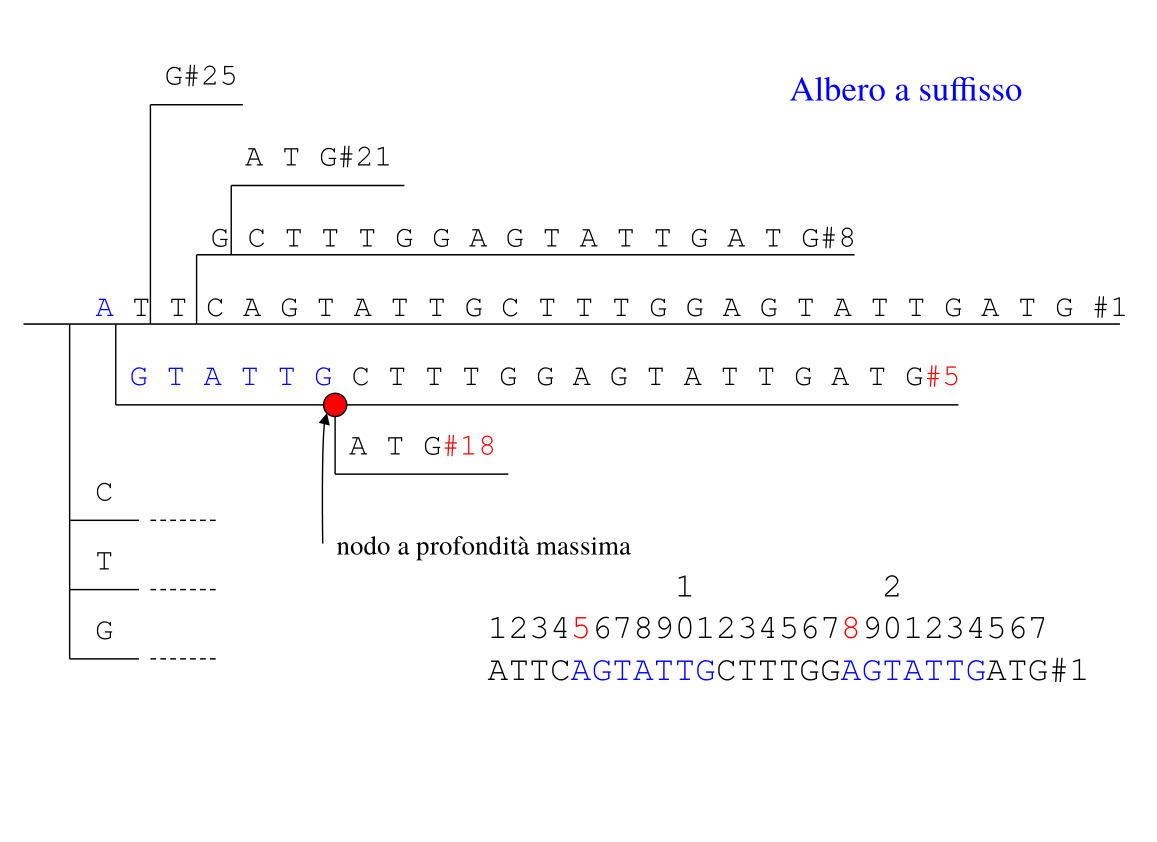
\includegraphics[ width=1.0\linewidth, height=\textheight, keepaspectratio]{./pics/alberi-suffisso.jpg}
    \caption{Schema di un albero a suffisso.}
    \label{fig:alberi-suffisso}
\end{figure}



\subsection{Il problema dei legami A-T e C-G e del ripiegamento delle proteine o del t-RNA}

Il DNA ha una struttura ``a scala'' o ``a doppia elica'' --- nella struttura vi
è una \emph{complementarietà} fra guanina e citosina, e adenina e tiamima. Le
due catene saranno (e devono essere) complementari, perciò la doppia catena
avrà un \emph{verso} che va da $5^\prime$ a $3^\prime$.

Il terzo problema è dunque quello del \textbf{ripiegamento delle proteine o del
t-RNA}. Data la sequenza primaria, bisogna determinare la struttura secondaria,
cioè trovare mediante la complementarietà A-T, G-C la stringa secondaria ad essa
associata. Bisognerà dunque determinare con tecniche informatiche la maniera in
cui la sequenza si ``ripiega'' su se stessa. 

\begin{figure}[ht]
    \centering
    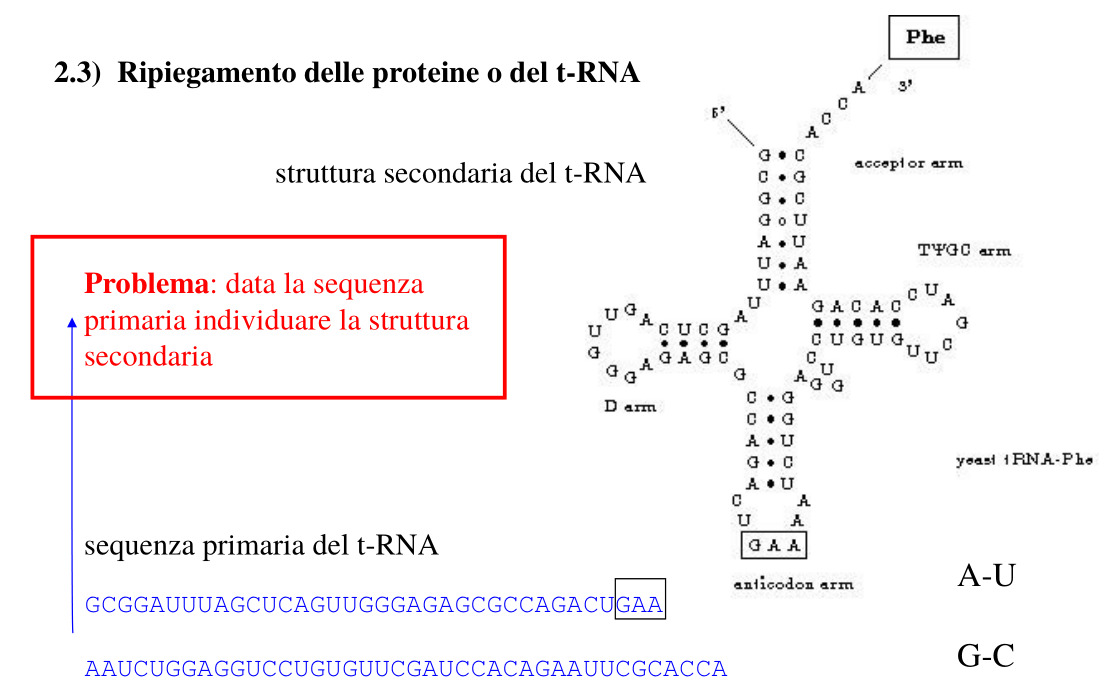
\includegraphics[ width=1.0\linewidth, height=\textheight, keepaspectratio]{./pics/struttura-trna.jpg}
    \caption{Struttura di uno t-RNA.}
    \label{fig:struttura-trna}
\end{figure}



Il medesimo problema si ha, ad esempio, per il ripiegamento della proteina
(ancor più difficile, poiché presentano ripiegamenti senza complementarietà e
tridimensionali).

\subsection{La costruzione di alberi filogenetici}

La costruzione degli \emph{alberi filogenetici} è un problema di distanza fra
stringhe proteiche. Si può adoperare la distanza di Levenshtein per determinare
se due sequenze hanno un \emph{avo comune}, cioè se ambedue le sequenze
derivano da una sequenza ancestrale. In altre parole, si individua una misura
di distanza fra stringhe che sia anche \emph{biologicamente significativa}.

\begin{figure}[ht]
    \centering
    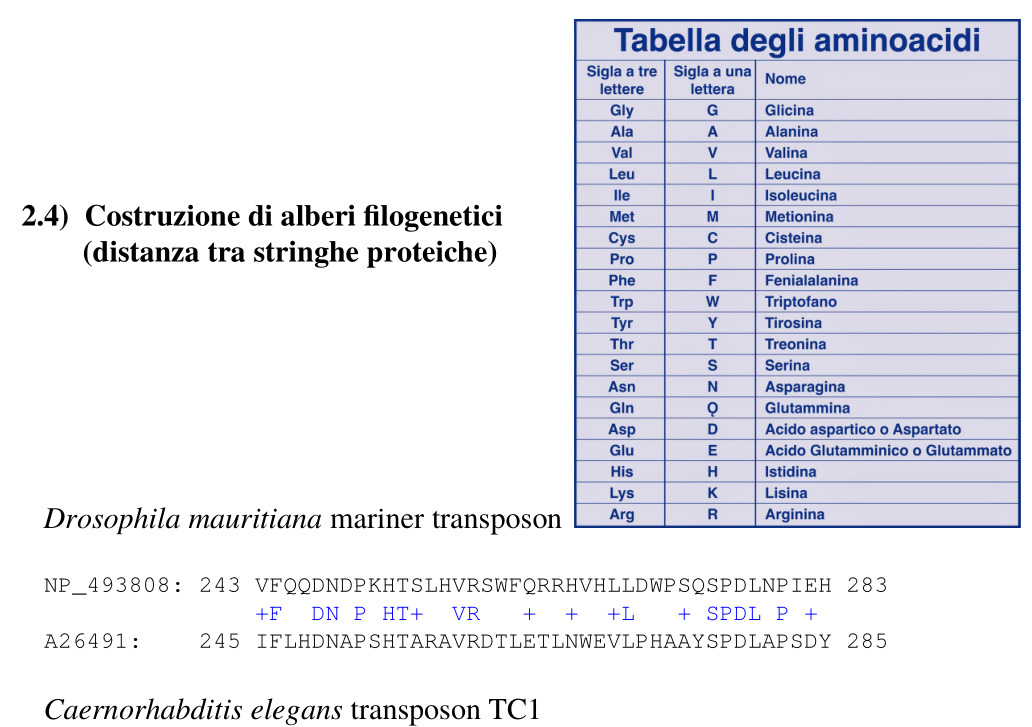
\includegraphics[ width=1.0\linewidth, height=\textheight, keepaspectratio]{./pics/alberi-filogenetici.jpg}
    \caption{Tabella degli amminoacidi per ricostruzione di alberi filogenetici. In particolare, vengono analizzate sequenze di \emph{drosophila mauritiana} e di \emph{caernorhabditis elegans}.}
    \label{fig:alberi-filogenetici}
\end{figure}

I trasposoni (le sequenze) vengono allineate, e si effettua una ricerca
approssimata per rilevare le somiglianze fra le due stringhe. Le somiglianze
possono essere sia \emph{esatte}, cioè porzioni di stringhe sono allineate e
identiche fra le due stringhe, oppure presentare \emph{amminoacidi affini}
(indicati con un $+$). Gli amminoacidi imparentati presentano un grado di
parentela, espresso nella \textbf{Matrice BLOSUM}. La Matrice BLOSUM contiene
un valore intero associato ad ogni coppia di amminoacidi --- tanto più alto il
valore associato alla coppia, tanto più la coppia sarà biologicamente affine.
La somma completa di parentela fra tutti gli amminoacidi dei trasposoni
conferisce un punteggio globale BLOSUM, da interpretare tramite conoscenze
di Biologia.


\begin{figure}[ht]
    \centering
    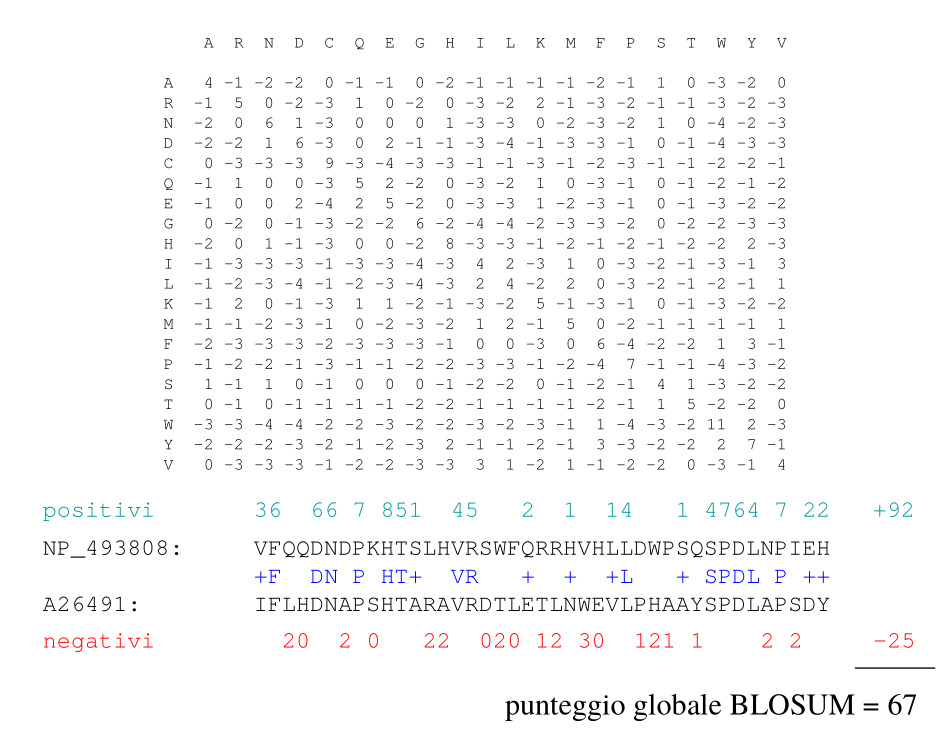
\includegraphics[ width=1.0\linewidth, height=\textheight, keepaspectratio]{./pics/matrice-blosum.jpg}
    \caption{Matrice BLOSUM per la ricostruzione in Figura~\ref{fig:alberi-filogenetici}. Ogni coppia di amminoacidi ha un valore intero positivo o negativo. Una somma sufficientemente positiva garantisce una buona corrispondenza per catene di proteine, e dunque la presenza di un avo comune.}
    \label{fig:matrice-blosum}
\end{figure}





\section{La computazione mediante DNA}

Le dimensioni di DNA e proteine sono estremamente ridotte: in poche frazioni di
millimetro cubo è infatti possibile immagazzinare una quantità enorme di
informazione sotto forma di sequenze di simboli. Tanto minori saranno le
dimensioni richieste dal DNA, tanto maggiori saranno le capacità computazionali
di tale sistema. Il trucco sarà prima di sfruttare la cellula --- molto
efficiente nella gestione di A, C, G, T --- per immagazzinare l'informazione, e
successivamente di adoperare il calcolatore e tecniche informatiche per
manipolare successivamente le sequenze di simboli.

Adleman propose nel 1994 un metodo per la costruzione di un \textbf{calcolatore
biomolecolare}, basato su un modello di computazione \emph{non} algoritmico
procedurale, benché il paradigma sia lo stesso (ricerca esauriente).

\subsection{Il problema del cammino Hamiltoniano su un grafo}

Il problema del cammino Hamiltoniano su un grafo è esprimibile nella seguente
maniera: dato un grafo con $n$ vertici, $v_1, v_2, \dots, v_n$ ed $m$ archi,
fissati due vertici di inizio e fine $v_i$ e $v_f$, verificare se esiste un
cammino che va da $v_i$ a $v_f$ con $n-1$ archi che tocchi ciascun vertice una
ed una sola volta.

Per il problema del cammino Hamiltoniano \textbf{non sono noti} algoritmi
efficienti: resta soltanto la soluzione bruta, cioè generare tutte le $(n-2)!$
permutazioni dei vertici, escludendo $v_i$ e $v_f$, e verificare l'esistenza
della soluzione. Inoltre,

$$n! \sim \sqrt{2} \pi \sqrt{n} e^{-n} n^n,$$

il che evidenzia che è un problema praticamente intrattabile con $n$ grande,
poiché anche i migliori algoritmi hanno complessità minima dell'ordine di
$2^n$. Già infatti con $n = 85$, si ottiene una complessità di $2^{85} = 3,86
\cdot 10^{25} op$, le quali richiedono oltre un miliardo di anni operando
$10^9$ operazioni al secondo!

La soluzione adottata per il problema del cammino Hamiltoniano è la seguente
\begin{enumerate}
    \item si codificano nodi ed archi in sequenze di DNA;
    \item si generano catene di DNA casuali, ciascuna di esse sarà associata ad
        un percorso --- ciò si fa lasciando le sequenze in un contenitore
        archi-vertici, con l'aggiunga dell'\emph{enzima Ligasi};
    \item si prendono soltanto quelli con il giusto nodo d'inizio $v_i$ e
        finale $v_f$, si scartano gli altri poiché fondamentalmente errati --
        ciò è realizzato mediante \emph{polymerase chain reaction};
    \item si trattengono tutti quelli che visitano $n$ vertici --- mediante
        \emph{elettroforesi con gel di agarosio}\footnote{La gelatina di
        agarosio (uno zucchero), se sottoposta a differenza di potenziale, fa
    sì che le molecole si polarizzino e si muovano all'interno del gel. Per via
della viscosità del gel, le molecole più corte viaggiano più velocemente,
mentre le molecole maggiormente lunghe saranno complessivamente più lente. Dopo
un lasso di tempo si può controllare il posizionamento delle molecole, che
formeranno agglomerati e saranno disposte in cluster a seconda della lunghezza.
Ecco che così facendo si potrà discernere fra i percorsi ``troppo lunghi'' e
``troppo corti'' e quelli della lunghezza corretta, che saranno collocati nello
stesso cluster.};
    item si trattengono solo quelli che visitano ciascun vertice almeno una
        volta --- si formano singoli strand di DNA accoppiati con tutti i
        vertici;
    \item i cammini rimanenti sono \emph{la soluzione} --- estratti in
        laboratorio.
\end{enumerate}

\begin{figure}[ht]
    \centering
    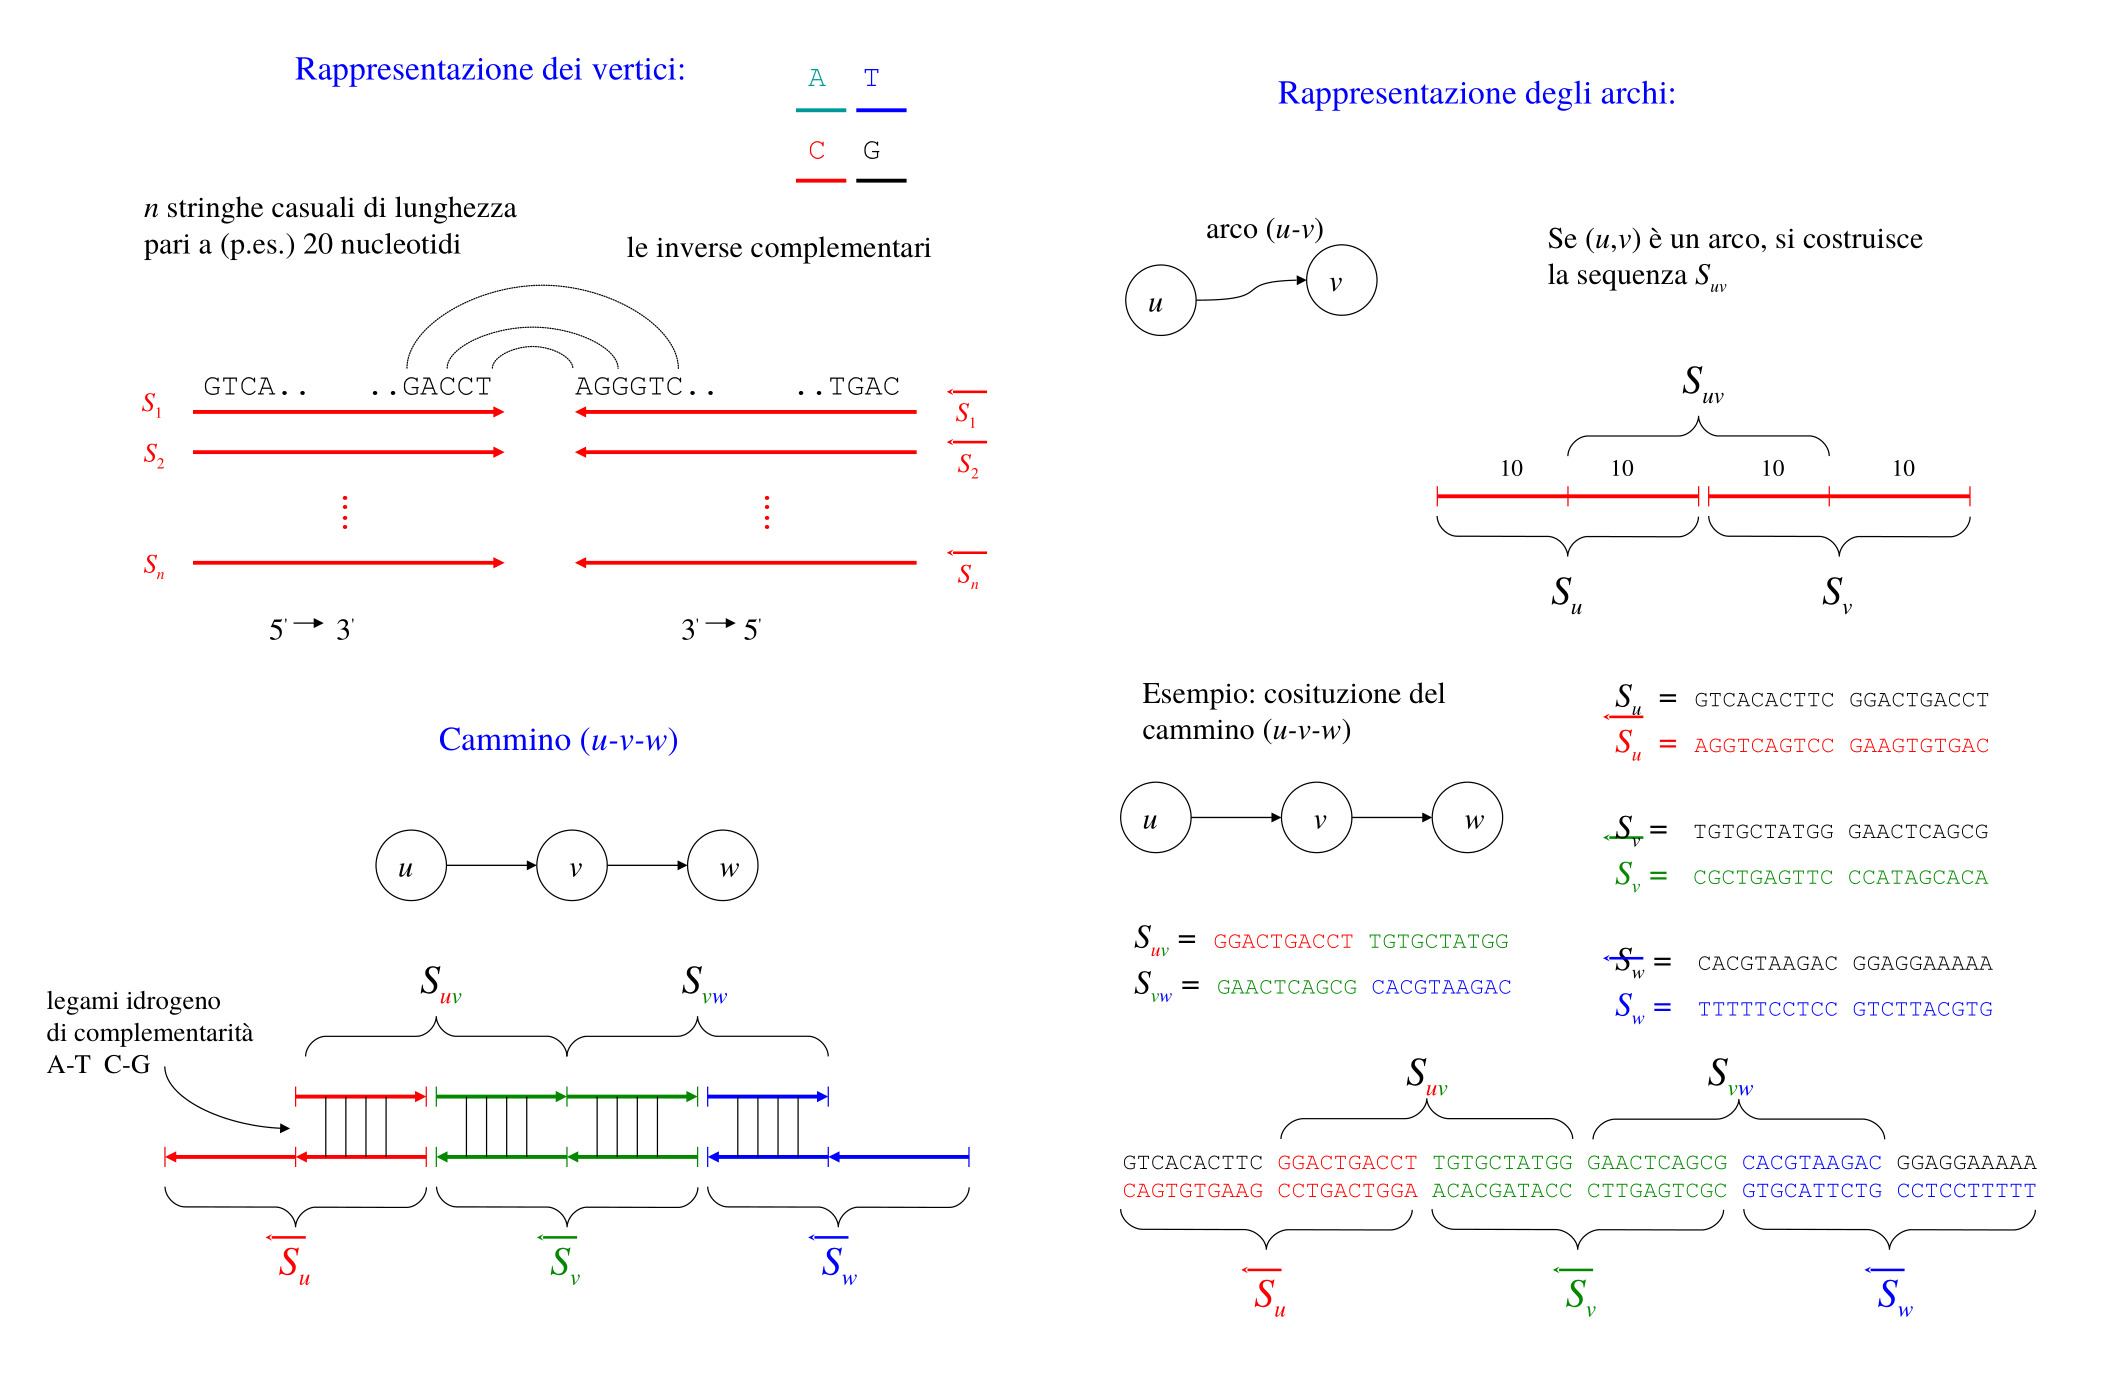
\includegraphics[ width=1.2\linewidth, height=\textheight, keepaspectratio]{./pics/computazioneDNA.jpg}
    \caption{La computazione DNA. Da sinistra a destra, dall'alto in basso: rappresentazione dei vertici mediante sequenze inverse complementari; rappresentazione degli archi con sequenze a metà fra due sequenze; catena di archi-nodi; dopo il mescolamento dei contenitori di archi e vertici, creazione del cammino u-v-w.}
    \label{fig:computazioneDNA}
\end{figure}



Per costruire i \emph{vertici} si determinano stringhe casuali assieme alle loro
inverse complementari. Supponiamo di costruire $n$ stringhe casuali di
lunghezza pari a $20$ nucleotidi, da $5^\prime$ a $3^\prime$. Il primo passo è
quello di determinare le stringhe \emph{inverse complementari}, cioè quelle da
sovrapporre e tali che $3^\prime \rightarrow 5^\prime$: le due stringhe
potranno incollarsi, poiché complementari.

Per costruire gli \emph{archi} $u\rightarrow v$ $S_{uv}$, si procede costruendo
una stringa di lunghezza $20$ con la coda del nodo $u$ ($S_u$) e con la testa del nodo
$v$ ($S_{v}$).

Si generano dunque moltissime (milioni di) copie delle $\overline{S}_j$
complementari e si mettono nel \emph{contenitore dei vertici}, mentre si
generano moltissime (anch'esse milioni di) copie delle $S_{uv}$, ponendole nel
\emph{contenitore degli archi}. Per la computazione, semplicemente, \emph{si
mescolano i contenitori}, e se per caso le sequenze si attaccano le une le altre,
queste formano una sequenza di vertici e nodi: abbiamo dunque realizzato la
seconda fase di generazione casuale dei percorsi.

Supponiamo di veder realizzato il cammino u-v-w. Gli archi sono costituiti con
metà di entrambi i nodi, mentre i vertici sono casualmente generati. Nel
contenitore dei DNA le sequenze possono muoversi liberamente, ed incrociarsi a
seconda delle affinità: può crearsi, in definitiva, una catena come in
Figura~\ref{fig:computazioneDNA}.

\subsection{I vantaggi e le limitazioni delle tecniche a computazione DNA}

I vantaggi \emph{teorici} principali sono legati alla \emph{velocità di
computazione}, milioni di volte più rapida dei computer tradizionali,
all'\emph{efficienza energetica} di miliardi di volte maggiore, e specialmente
alla capacità di \emph{memorizzazione ad altissima densità} (miliardi di
volte maggiore). Infatti, $1cm$ cubo può contenere fino a $10000$ mld di
molecole di DNA; $1$ bit è contenuto in $1nm$ cubo col DNA, mentre in $10^{12}nm$
cubi con CD. Un calcolatore DNA potrebbe gestire $10TB$ di memoria con una
velocità di calcolo di $10^{13}$ operazioni al secondo.

Le limitazioni sono purtroppo pesantissime: il numero di molecole implicate è
lo stesso delle soluzioni possibili nella ricerca esauriente, cioè all'incirca
$\sim 2^n$. Purtroppo, scegliendo $n=100$ il peso del DNA sarebbe superiore a
$10t$, mentre con $n=200$ il totale peso delle stringhe richieste sarebbe
superiore al peso della Terra!

L'altra limitazione sono le \emph{imperfezioni nelle tecniche di sintesi del
DNA}, comportando una presenza non trascurabile di errori. Inoltre, il
bio-calcolatore deve essere \emph{dedicato al problema}, ed il \emph{tempo} di
ogni operazione biologica richiede ore o giorni. In altre parole, la
complessità temporale viene sostituita con la \textbf{complessità sul peso}.


\chapter{Teoria degli automi e dei linguaggi formali}

Gli \textbf{automi a stati finiti} sono la classe delle macchine con minore
potenza computazionale.

Un automa a stati finiti può essere rappresentato mediante una testina che si
muove su un nastro contenente dei simboli e potenzialmente illimitato, sempre
nella stessa direzione. La testina può trovarsi in un certo \emph{stato} --- a
seconda dello stato $q$ e del simbolo $s_i$ letto sul nastro, la testina si
porta in un altro stato o rimane nello stesso in cui si trovava, per poi
spostarsi a destra per apprestarsi a leggere il simbolo successivo.

\begin{figure}[h]
    \centering
    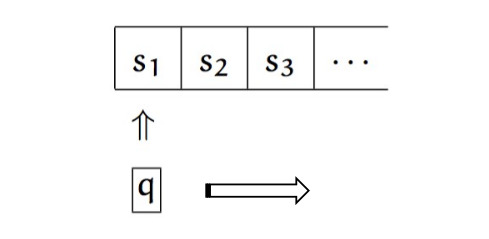
\includegraphics[ width=0.5\linewidth, height=\textheight, keepaspectratio]{./pics/automaStatiFiniti.jpg}
    \caption{Rappresentazione schematica di un automa a stati finiti.}
    \label{fig:automaStatiFiniti}
\end{figure}

Quando la lettura dei simboli termina, a seconda dello stato raggiunto dalla
testina, l'automa fornisce un risultato di \emph{accettazione} o di
\emph{refutazione} della stringa.

Fra le macchine concepibili, le macchine a stati finiti sono le meno potenti.
Volendole classificare in base alle caratteristiche e alle loro possibilità:
\begin{description}
    \item[Macchina di Turing] può leggere e scrivere a destra e sinistra della
        stringa;
    \item[Macchina di Post] legge a sinistra, mentre scrive ed allunga la
        stringa a destra;
    \item[Macchine con memorie push-down] leggono a sinistra di $x$,
        leggono e scrivono a sinistra di ciascuna memoria push-down. Le
        macchine con memorie push-down hanno differenti potenze computazionali
        a seconda del numero di tali memorie;
    \item[Automi, macchine a stati finiti] leggono a sinistra, non possono
        scrivere. Eseguono essenzialmente delle \emph{letture}, ma non delle
        scritture.
\end{description}

Gli automi non sono perciò in grado di scrivere qualcosa sul nastro. La memoria
a disposizione sull'automa è una qualche sorta di \emph{memoria di sola
lettura} --- il nastro supporta esclusivamente la stringa $x$, di lunghezza
comunque finita. Un automa, dunque, può essere considerato come una macchina
che svolge compiti in base alle istruzioni fornite sul nastro, oppure come una
macchina che riconosce stringhe. Ci ritroviamo dunque in una situazione del
tutto simile a quanto accadeva per la macchina di Turing, con la sola
differenza che un automa è in grado di riconoscere un numero molto più limitato
di stringhe.

\section{I linguaggi regolari}

La \textbf{chiusura (o stellatura)} $S^*$ dell'insieme $S$ è l'insieme
costituito dalla parola vuota e da tutte le parole formate concatenando un
numero finito di parole in $S$, cioè quindi

$$S^* = S^0 \cup S^1 \cup S^2 \cup \dots$$
dove $S^0 = \{\Lambda\},$ e $S^i=S^{i-1}S, i > 0$, con $\Lambda$ \emph{parola vuota}.

Sia $\Sigma = \{a, b\}$ un alfabeto di simboli (contenente in questo caso due
simboli), $\Lambda$, e sia la \textbf{stellatura
dell'insieme} $\Sigma^* = \{\Lambda, a, b, aa, ab, ba, bb, aaa, aab, \dots\}$
definiamo il \textbf{prodotto (concatenazione)} $UV$ di due sottoinsiemi $U, V$
di $\Sigma^*$ come l'insieme

$$UV = \{x | x= uv, u \in U, v \in V\}.$$

In altre parole, ogni parola dell'insieme $UV$ è formata concatenando una
parola di $U$ con una parola di $V$. Prendendo due sottoinsiemi $U=\{a, ab,
aab\}$ e $V=\{b, bb\}$ allora l'insieme $UV = \{ab, abb, abbb, aabb, aabbb\}$.
In generale, il prodotto non è commutativo, nel senso che l'insieme ottenuto
potrebbe non essere uguale. L'operazione prodotto è tuttavia associativa, cioè
per qualunque $U, V, W \in \Sigma^*$ si ha che $(UV)W = U(VW)$.

Esaminiamo ora la classe degli \textbf{insiemi regolari}. La classe degli insiemi regolari su $\Sigma$ è ricorsivamente definita come segue:
\begin{enumerate}
    \item ogni insieme \emph{finito} di parole su $\Sigma$, compreso l'insieme
        vuoto $\emptyset$, è un insieme regolare;
    \item se $U$ e $V$ sono insiemi regolari su $\Sigma$, lo sono anche la loro
        unione $U\cup V$ ed il loro prodotto $UV$;
    \item se $S$ è un insieme regolare su $\Sigma$, lo è anche la sua chiusura
        $S^*$.
\end{enumerate}

Dunque nessun insieme è regolare, a meno che non possa essere ottenuto con un
numero finito di applicazione dei punti 1, 2 o 3, applicando cioè la ricorsione dei tre elementi di cui sopra. Perciò, la classe degli
insiemi regolari su $\Sigma$ è la più piccola classe che contiene tutti gli
insiemi finiti di parole su $\Sigma$, e che è al contempo chiusa rispetto ad
unione, prodotto e stellatura dell'insieme.

Gli insiemi regolari sono generalmente molto semplici sia nella loro formazione che nella loro trattazione. Si può dimostrare che un sottoinsieme di
$\Sigma^*$ è regolare \emph{se e solo se}

\begin{enumerate}
    \item è accettato da qualche \emph{automa finito};
    \item è accettato da qualche \emph{grafo di transizione} --- una
        definizione differente di un automa a stati finiti, del tutto analoga;
    \item può essere espresso da qualche \emph{espressione regolare}.
\end{enumerate}

Le espressioni regolari sono, in ultima analisi, quelle che riescono ad
esprimere stringhe appartenenti ad insiemi regolari. Esempi di espressioni
regolari sono l'insieme di tutte le parole di $\Sigma = \{a, b\}$ che
contengono o due $a$ consecutive, o due $b$ consecutive, e l'insieme delle
parole di $\Sigma$ che contengono un numero pari di $a$ e pari di $b$. Al
contrario, l'insieme $\{a^n b^n| n\geq 0\}$ \emph{non} è un imsieme regolare su
$\Sigma$, poiché non può essere accettato da un automa a stati finiti, e dunque nemmeno da un grafo di transizione o essere espresso tramite espressioni regolari, come è stato mostrato nelle sezioni precedenti.

\section{Gli automi}

Un esempio concreto di automa a stati finiti può essere un controllore di un comune portone elettrico.
La funzionalità dell'automa è \emph{insita nei suoi stati}: il cancello può essere
nello stato di \textsc{Aperto } oppure nello stato di \textsc{Chiuso}, rappresentando le
corrispondenti condizioni in cui può trovarsi il portone. Vi sono quattro possibili condizioni di
input per la posizione di persone, dipendenti dalla posizione di esse relativamente al cancello:
\textsc{Fronte}, \textsc{Retro}, \textsc{Entrambi}, \textsc{Nessuno}.

\begin{figure}[h]
    \centering
    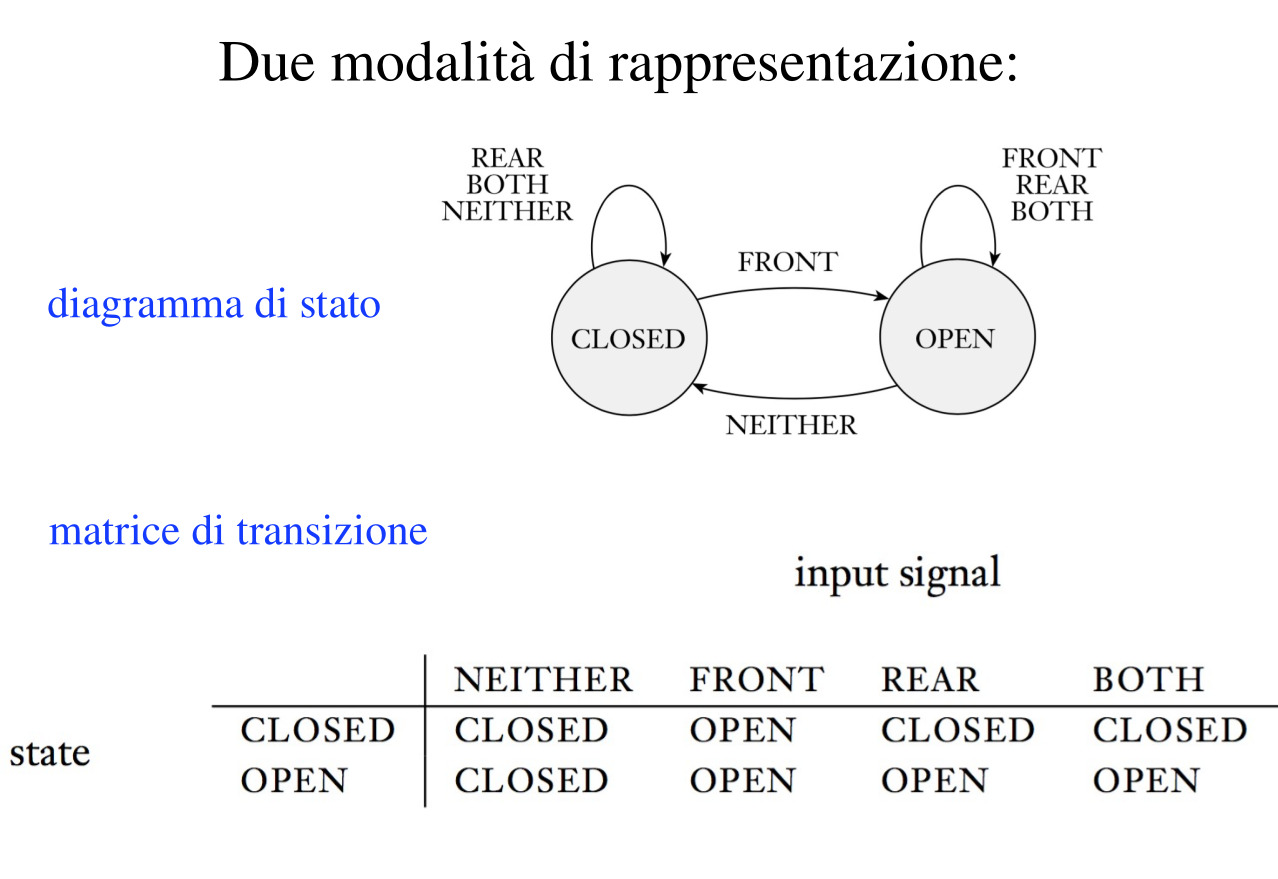
\includegraphics[ width=1.0\linewidth, height=\textheight, keepaspectratio]{./pics/automaStatiFinitiCancello.jpg}
    \caption{Doppia modalità di rappresentazione per un automa a stati finiti.
    Esso può essere rappresentato o come \emph{diagramma di stato}, o come
\emph{matrice di transizione}.}
    \label{fig:automaStatiFinitiCancello}
\end{figure}

Vi sono due possibili rappresentazioni per un automa: la prima è mediante il
\textbf{diagramma di stato}, la seconda attraverso la sua \textbf{matrice di
transizione}. È importante precisare la differenza fra quest'ultima e la matrice della macchina di
Turing: negli automi non è prevista un'operazione di scrittura da svolgere alla
lettura di un simbolo. Il sistema è infatti capace solo di transitare verso uno
stato successivo, non di effettuare operazioni di scrittura su memorie o di immagazzinare
informazioni.

\begin{figure}[h]
    \centering
    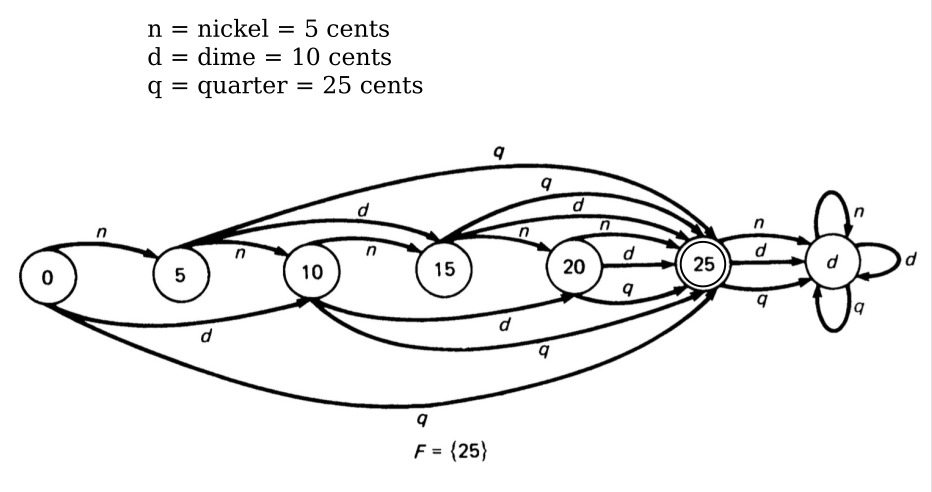
\includegraphics[ width=1.0\linewidth, height=\textheight, keepaspectratio]{./pics/automiVendingMachine.jpg}
    \caption{Macchina per la distribuzione di caramelle negli Stati Uniti, dal
    costo di 25 cents. Se vengono inseriti più di 25 cents, la macchina non dà
resto.}
    \label{fig:automiVendingMachine}
\end{figure}

Siamo ora pronti a fornire la prima definizione di automa a stati finiti.
\begin{definizione}[Automa finito 1]
Un \textbf{automa finito} A su $\Sigma$, dove $\Sigma = \{\sigma_1, \sigma_2,
\dots, \sigma_n\}$ è un grafo finito orientato in cui da ogni vertice escono
$n$ archi, con ogni arco etichettato con un diverso $\sigma_i$, con $1 \leq i
\leq n$. Esiste un vertice, etichettato con il segno $-$, detto \emph{vertice
iniziale}, ed un insieme di vertici eventualmente vuoto etichettati con un
segno $+$, detti \emph{vertici finali}, con la possibilità che il vertice
iniziale sia anche un vertice finale. Talvolta i vertici sono chiamati
\textbf{stati}.
\end{definizione}


La seconda definizione di automa finito è più formale, ed equivalente alla
precedente.

\begin{definizione}[Automa finito 2]
Un \textbf{automa finito} è una $5$-tupla $\mathcal Q, \Sigma, \delta, q_0,
\mathcal F)$ dove 
\begin{enumerate}
    \item $\mathcal Q$ è un insieme finito di \emph{stati};
    \item $\Sigma$ è un insieme finito, detto \emph{alfabeto};
    \item $\delta : \mathcal Q \times \Sigma \rightarrow \mathcal Q$ è la
        \emph{funzione di transizione};
    \item $q_0$ è lo \emph{stato di partenza};
    \item $\mathcal F \subset \mathcal Q$ è l'\emph{insieme degli stati
        di accettazione}.
\end{enumerate}
\end{definizione}

\begin{figure}[h]
    \centering
    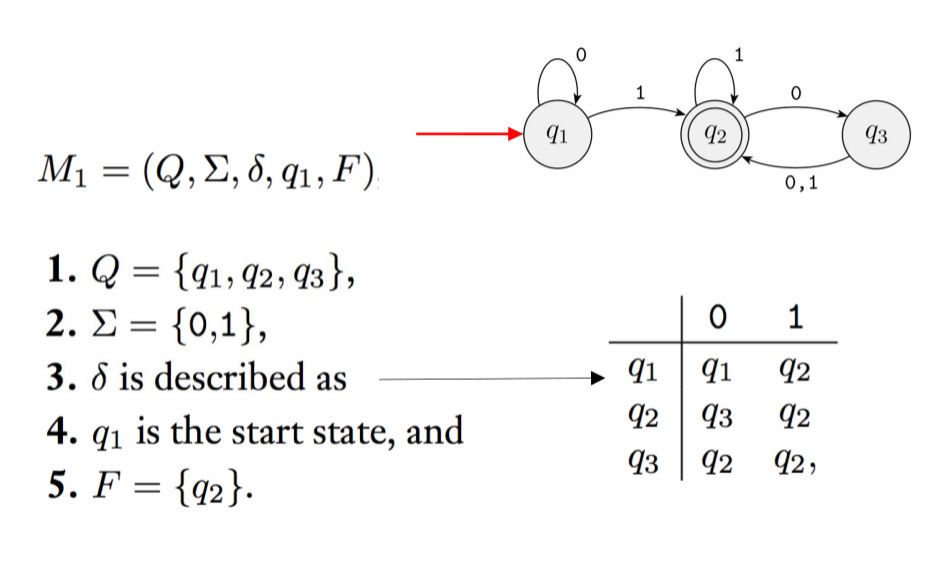
\includegraphics[ width=1.0\linewidth, height=\textheight, keepaspectratio]{./pics/wwAutoma.jpg}
    \caption{Automa a stati finiti che riconosce le stringhe A = \{w | w \mbox{ contiene almeno un } 1\mbox{ ed un numero pari di } 0 \mbox{ seguono l'ultimo } 1\}}
    \label{fig:wwAutoma}
\end{figure}

Un'importante nozione è quella di \emph{linguaggio della macchina}. Se $A$ è
l'insieme di tutte le stringhe accettate dalla macchina $M$, si dice che $A$ è
il \textbf{linguaggio della macchina} $M$, e scriviamo $\mathcal L(M) = A$. Ciò
che un automa a stati finiti accetta rientra perciò nel suo linguaggio.
Nell'esempio di cui sopra, $$\mathcal L(M) = A = \{w | w \mbox{ contiene almeno
un } 1 \mbox{ ed un numero pari di } 0 \mbox{ seguono l'ultimo } 1\}.$$

\begin{figure}[h]
    \centering
    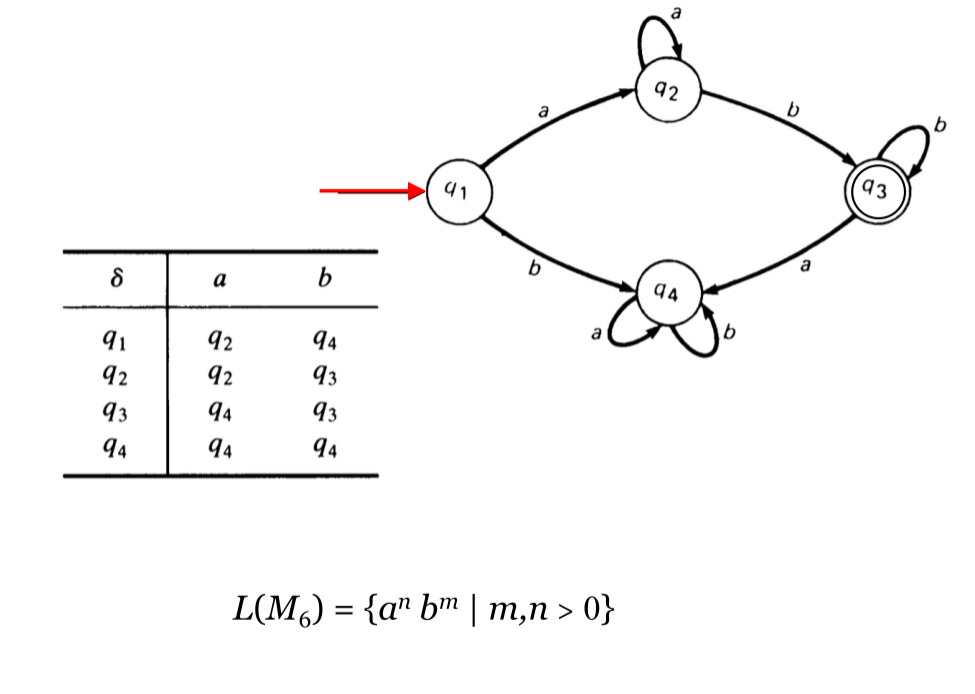
\includegraphics[ width=1.0\linewidth, height=\textheight, keepaspectratio]{./pics/automaAnBm.jpg}
    \caption{Automa a stati finiti che riconosce qualsiasi stringa della forma
    $\mathcal L(M) = \{a^n b^m | m,n > 0\},$ ma \textbf{non} stringhe della
forma $a^n b^n$ con $n>0$.}
    \label{fig:automaAnBm}
\end{figure}



\section{La computazione degli automi deterministici (DFA) dal punto di vista formale}

Sia $A_D = \{ \mathcal Q, \Sigma, \delta_D, q_0, \mathcal F\}$, con $\delta_d:\mathcal Q \times \Sigma \rightarrow \mathcal Q$ funzione di transizione. Se $x\in
\Sigma^*$ viene introdotto $\hat{\delta}_D (q, x)$ lo \textbf{stato raggiunto} da
$M$ partendo da $q$ quando si è alla sinistra di $x$, ed eseguendo
successivamente il cammino $x$.

Lo stato raggiunto può essere definito per ricorsione. Infatti,

$$
\left\{
    \begin{array}{l}
        \hat{\delta}_D (q, \Lambda) = q \\
        \hat{\delta}_D (q, xa) = \delta _D (\hat{\delta}_D (q, x), a)
    \end{array}
\right.
$$

con $\delta_D(q, a) = \hat{\delta}_D(q, a)$. In altre parole, l'automa deterministico $A_D$ accetta una
parola $x$ se $\hat{\delta}(q_0, x) \in \mathcal F$ appartiene all'insieme degli stati di
accettazione, ovvero $$\mathcal L(A_D) = \{x\in \Sigma^* | \hat{\delta}(q_0, x)
\in \mathcal F\}.$$ In definitiva, uno stato di \textsc{Accettazione } viene
raggiunto dallo stato iniziale $q_0$ solo se lo stato raggiunto da $q_0$
mediante un cammino $x$ conduce proprio allo stato di \textsc{Accettazione },
cioè quando $\hat{\delta}(q_0, x)$ appartiene all'insieme degli stati finali (di
accettazione). Si dimostrerà che un linguaggio accettato da un automa a stati
finiti è un linguaggio \emph{regolare}: questo legame fra automi a stati finiti
e linguaggi regolari consente di trattare gli automi mediante il formalismo dei
linguaggio regolari.

\subsection{Gli automi non deterministici}

Un \textbf{automa non deterministico} (Non-deterministic Finite Automa) vede
rimosso il vincolo che da ciascun nodo escano tutti e solid $\Sigma$ caratteri
\emph{diversi} dell'alfabeto. Gli automi deterministici sono introdotti per
semplificare enormemente il grafo risultante. Solitamente, automi
deterministici producono grafi enormemente più complessi e meno sintetici
rispetto agli automi non deterministici.


\begin{figure}[ht]
    \centering
    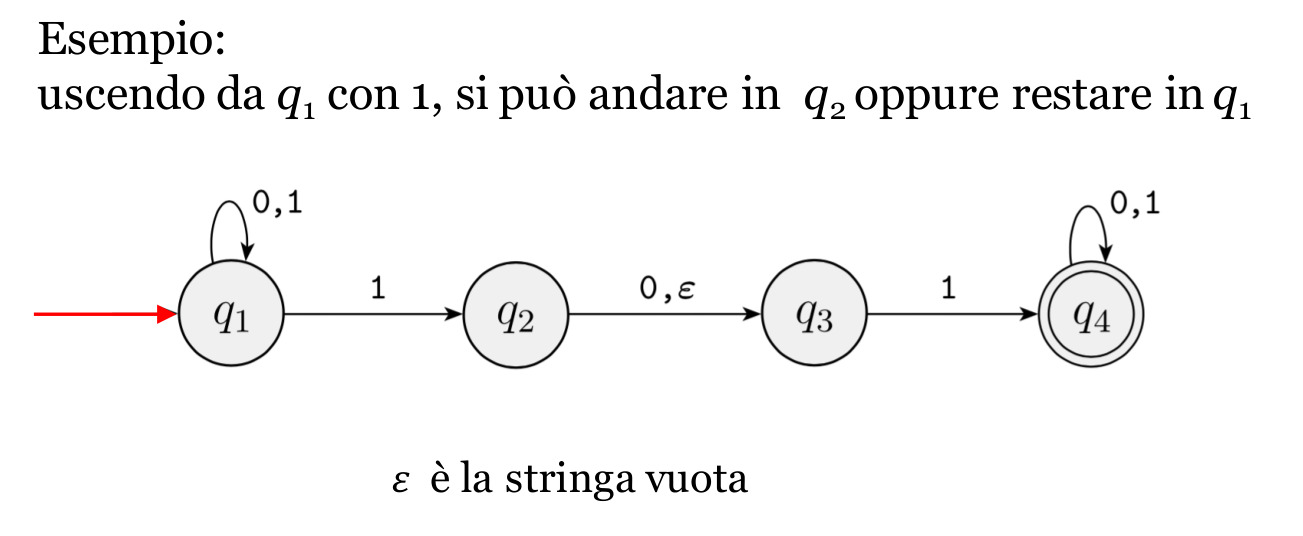
\includegraphics[ width=1.0\linewidth, height=\textheight, keepaspectratio]{./pics/nfa-intro.jpg}
    \caption{Esempio di automa a stati finiti non deterministico. Si osservi la semplicità del grafo.}
    \label{fig:nfa-intro}
\end{figure}

\begin{figure}[ht]
    \centering
    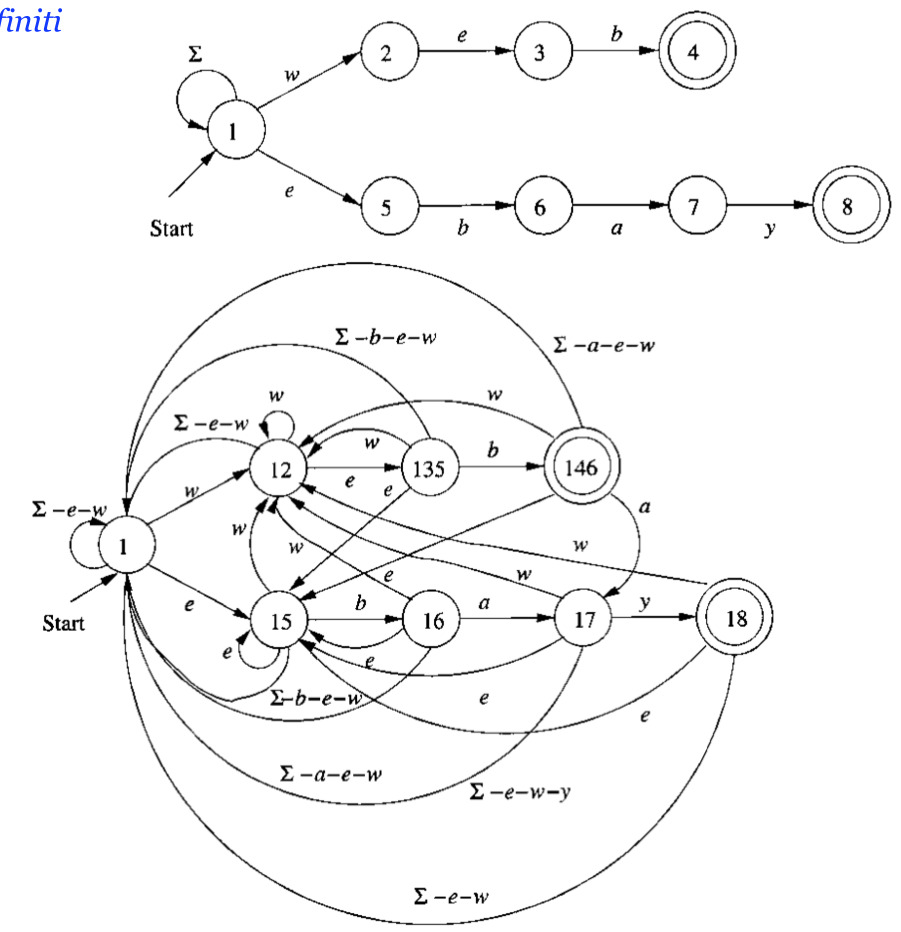
\includegraphics[ width=1.0\linewidth, height=\textheight, keepaspectratio]{./pics/nfa-esempio2.jpg}
    \caption{Paragone fra grafo risultante di un automa a stati finiti deterministico e quello di un automa non deterministico.}
    \label{fig:nfa-esempio2}
\end{figure}

\begin{figure}[ht]
    \centering
    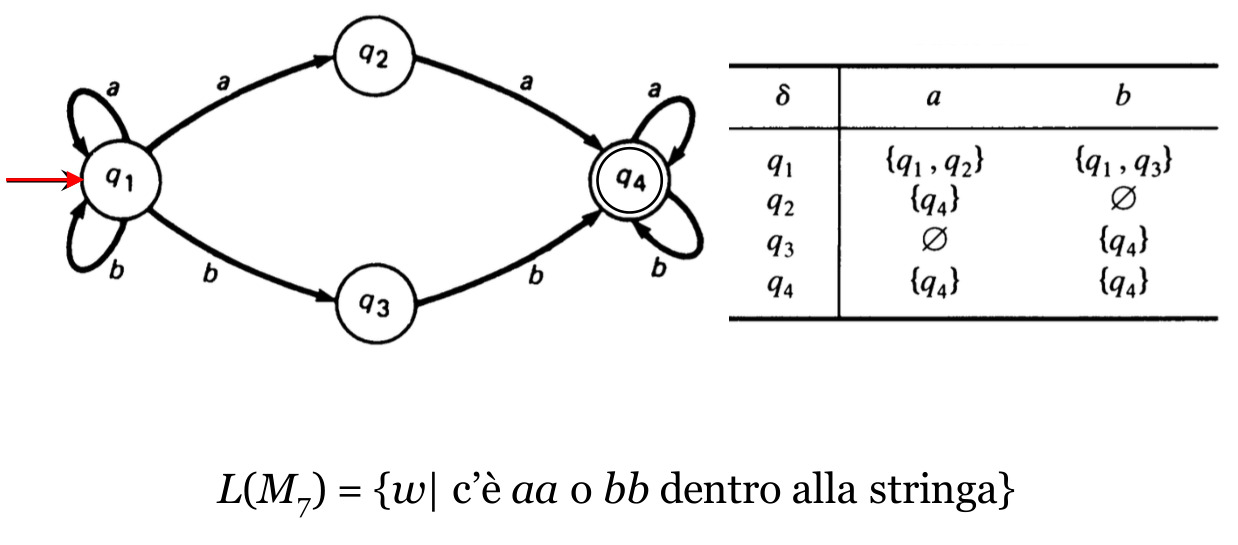
\includegraphics[ width=1.0\linewidth, height=\textheight, keepaspectratio]{./pics/nfa-esempio3.jpg}
    \caption{Esempio di un grafo con relativa tabella (funzione) di transizione.}
    \label{fig:nfa-esempio3}
\end{figure}





Il fatto di introdurre il non determinismo non introduce una maggiore potenza
computazionale, bensì funge esclusivamente da semplificazione notevole per la
rappresentazione a grafi.

\subsection{Equivalenza fra automi NFA ed automi DFA}

È possibile stabilire un'equivalenza fra automi a stati finiti di tipo
deterministico e di tipo non deterministico, a tal punto da fornire una regola
per trasformare un grafo di una tipologia al grafo dell'altra. Si supponga di
partire dal grafo di Figura~\ref{fig:equivalenza-nfa-dfa}, relativo ad un
automa che accetta tutte le stringhe che finiscono con \texttt{'01'}.

Si consideri il grafo relativo all'automa non deterministico. Per convertire in
un grafo relativo ad un automa deterministico, si procede nella seguente
maniera:
\begin{enumerate}
    \item come prima cosa, si esamina il grafo dell'automa non deterministico;
    \item in secondo luogo, si crea l'insieme degli stati. Gli stati di cui
        sarà dotato l'automa deterministico saranno gli stati dell'automa non
        deterministico con, in aggiunta, dei \textbf{macrostati} che descrivono
        tutte le possibili unioni degli stati precedenti. In altre parole,
        supponendo gli stati $q_0$, $q_1$ e $q_2$ dell'automa non
        deterministico, l'automa deterministico sarà dotato degli stati $q_0$,
        $q_1$ e $q_2$, assieme agli stati $\{q_0, q_1\}$, $\{q_0, q_2\}$,
        $\{q_1, q_2\}$ e $\{q_0, q_1, q_2\}$. Fra essi vi è compreso
        anche lo \emph{stato nullo} $\emptyset$, come mostrato in
        Figura~\ref{fig:equivalenza-nfa-dfa};
    \item per ciascuno degli stati e macrostati, si compila la tabella
        riportando il percorso a seconda dell'input. Ad esempio in
        Figura~\ref{fig:equivalenza-nfa-dfa} trovandosi nello stato $q_0$
        dell'automa non deterministico, a fronte di un ingresso 0 potremo
        muoverci o nello stato $q_0$ oppure nello stato $q_1$. Pertanto,
        rappresenteremo questa condizione nell'automa deterministico facendolo
        raggiungere lo stato $\{q_0, q_1\}$, ``rappresentativo'' di entrambi
        gli stati;
    \item se un input non è contemplato, il suo risultato sarà $\emptyset$. Gli
        stati iniziali si possono indicare con una freccia, quelli terminanti
        (di \textsc{Accettazione}) con un asterisco.
\end{enumerate}

Una volta completato questo processo osservando accuratamente il grafo
dell'automa non deterministico, otterremo un \emph{grafo equivalente}
dell'automa deterministico. Con tutta probabilità, esso sarà molto più
complesso ed elaborato, come mostra la Figura~\ref{fig:equivalenza-nfa-dfa2}.
Porzioni di grafo potrebbero non essere collegate ad alcuno stato iniziale (in
questo caso allo stato $q_0$) e sebbene facciano parte del grafo completo, esse
vengono tolte per attuare una semplificazione.

\begin{figure}[ht]
    \centering
    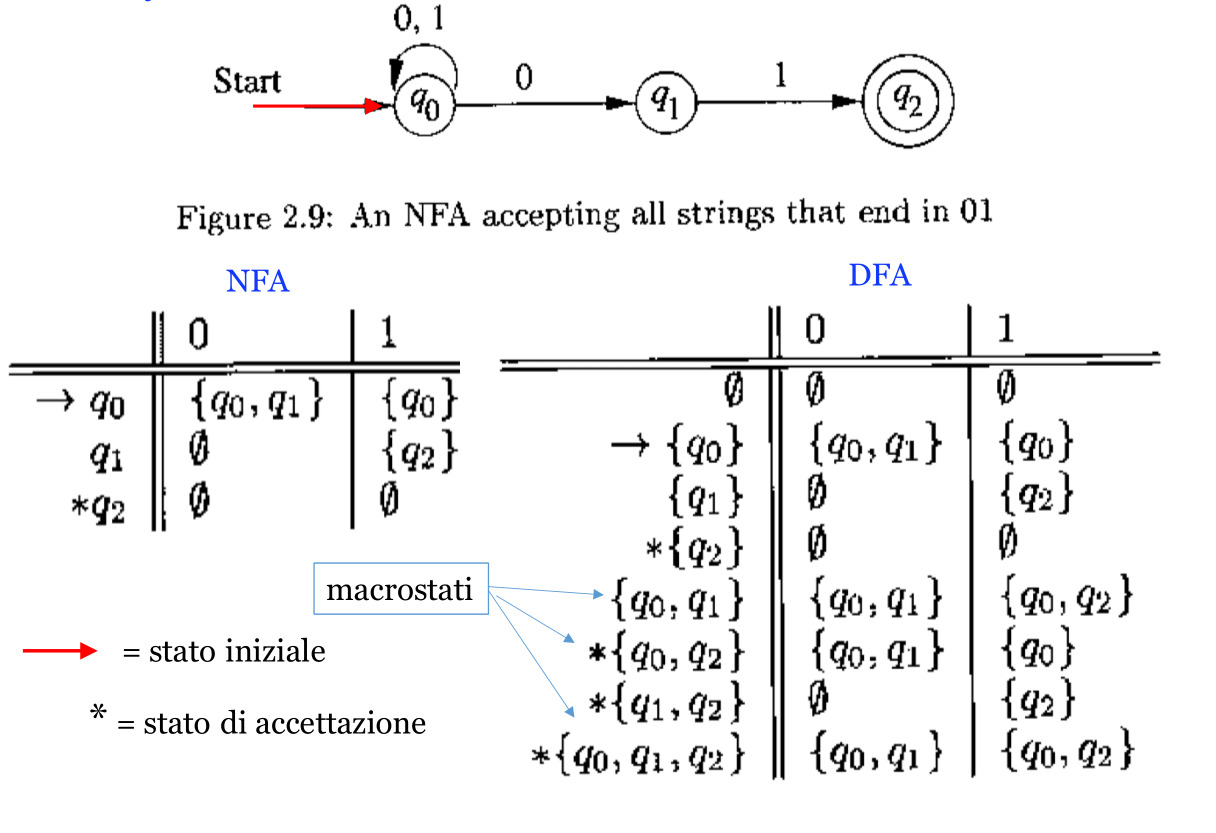
\includegraphics[ width=1.0\linewidth, height=\textheight, keepaspectratio]{./pics/equivalenza-nfa-dfa.jpg}
    \caption{Equivalenza fra automa a stati finiti non deterministico e fra uno deterministico.}
    \label{fig:equivalenza-nfa-dfa}
\end{figure}

\begin{figure}[ht]
    \centering
    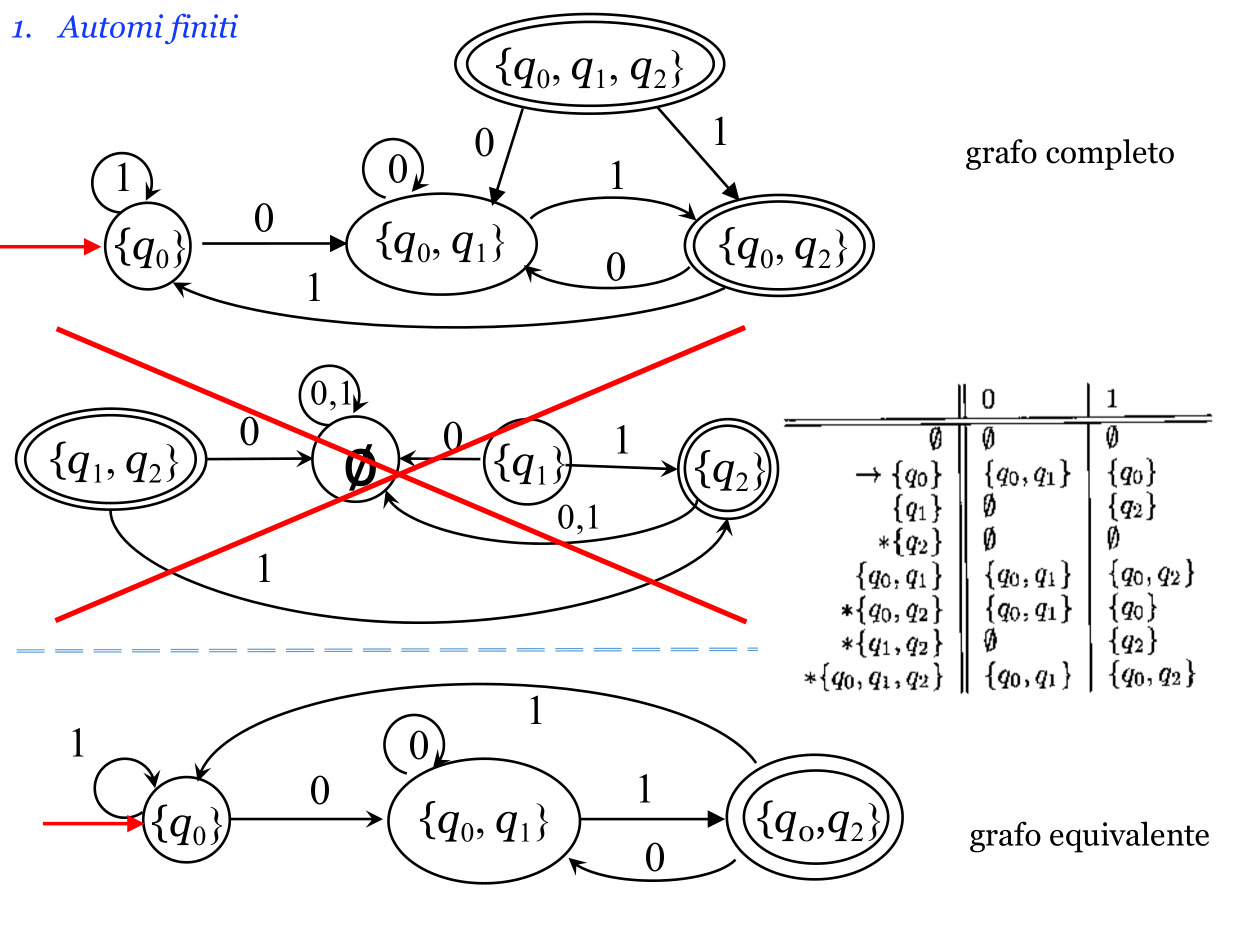
\includegraphics[ width=1.0\linewidth, height=\textheight, keepaspectratio]{./pics/equivalenza-nfa-dfa2.jpg}
    \caption{Grafo completo ed equivalente della Figura~\ref{fig:equivalenza-nfa-dfa}. La croce in rosso evidenzia la parte rimovibile, poiché non connessa con alcuno stato iniziale.}
    \label{fig:equivalenza-nfa-dfa2}
\end{figure}

\clearpage

\subsection{Automa non deterministico}

\begin{definizione}[Automa a stati finiti non deterministico]
Un \textbf{automa a stati finiti non deterministico} è una $5$-tupla $\mathcal Q, \Sigma, \delta, q_0,
\mathcal F)$ dove 
\begin{enumerate}
    \item $\mathcal Q$ è un insieme finito di \emph{stati};
    \item $\Sigma$ è un insieme finito, detto \emph{alfabeto};
    \item $\delta : \mathcal Q \times \Sigma \rightarrow \mathcal P(\mathcal Q)$ è la
        \emph{funzione di transizione};
    \item $q_0$ è lo \emph{stato di partenza};
    \item $\mathcal F \subset \mathcal Q$ è l'\emph{insieme degli stati
        di accettazione}.
\end{enumerate}
\end{definizione}

La differenza principale rispetto agli automi deterministici è la definizione
della funzione di transizione $\delta$, dove il codominio è l'\emph{insieme
delle parti} di $\mathcal Q$ anziché l'insieme $\mathcal Q$, come ci si può
aspettare. D'altronde, in un automa non deterministico un nodo di un grafo può disporre di
un numero arbitrario di collegamenti verso qualsiasi altro nodo, potenzialmente
verso tutti gli altri contemporaneamente.

Similmente, la computazione per automi non deterministici dal punto di vista
formale avviene con le seguenti differenze:

Sia $A_N = \{ \mathcal Q, \Sigma, \delta_D, q_0, \mathcal F\}$ un automa non
deterministico. Se $x\in \Sigma^*$ viene introdotto $\hat{\delta}_D (q, x)$
l'\textbf{insieme degli stati raggiunti}\footnote{Coerentemente a come abbiamo
definito l'automa a stati finiti non deterministico, questa volta lo stato
raggiunto a partire da un determinato nodo può produrre più possibili stati
come esito di un singolo input.} da $A_N$ partendo da $q$ quando si è alla
sinistra di $x$, ed eseguendo successivamente \emph{tutti i percorsi} $x$.

Di conseguenza, si può definire per ricorsione in modo analogo a quanto svolto prima:

$$
\left\{
    \begin{array}{l}
        \hat{\delta}_N (q, \Lambda) = \{q\} \\
        \hat{\delta}_N (q, xa) = \displaystyle \bigcup_{p \in \hat{\delta}_N(q, x)} \hat{\delta}_N (p, a)
    \end{array}
\right.
$$

Si avrà infine che $A_N$ accetta una parola $x$ se $\hat{\delta}_N(q_0, x) \cap F
\neq \emptyset$, cioè

$$L(A_N) = \{x \in \Sigma^* | \hat{\delta}_N(q_0, x) \cap F \neq \emptyset \}$$

in modo congruo a quanto visto per un automa $A_D$ deterministico.

Poiché ogni automa non deterministico può essere descritto da un automa
deterministico in cui la $\delta_N(q, x)$ restituisce un solo stato, ogni
linguaggio regolare è accettato da un automa non deterministico per via
dell'equivalenza che sussiste fra i due tipi di automi. Dunque, un linguaggio
accettato da un automa non deterministico risulterà sempre essere
un \emph{linguaggio regolare}. La dimostrazione di ciò è nelle dispense a
pagina 109 (Teorema dell'equivalenza NFA-DFA).

\section{Pumping lemma}

Un notevole risultato della teoria della computazione è famoso col nome di
\textbf{Pumping lemma}, detto anche \emph{lemma di espansione}.

\begin{thm}[Pumping lemma]
    Sia $\mathcal L = \mathcal L(\mathcal A)$, dove $\mathcal A$ è un automa a
    $m$ stati. Sia $x \in \mathcal L$, con $|x| \geq m$. Allora si può scrivere
    $x = uvw$, dove $v \neq \Lambda$ e $uv^{[i]}w \in \mathcal L$\footnote{La
    parte centrale della stringa è infinitamente replicabile, tuttavia il
risultato continua ad appartenere al linguaggio $\mathcal L$.} per tutti i
    valori $i = 0,1,2,3,\dots$.
\end{thm}

\textsc{Dimostrazione} --- Poiché $x$ consiste di almeno $m$ simboli,
$\mathcal A$ deve passare attraverso almeno $m$ transizioni di stato mentre
scansiona $x$; contando lo stato iniziale ciò richiede almeno $m + 1$ stati non
necessariamente distinti. Ma poiché in tutto ci sono soltanto $m$ stati,
concludiamo (per il \emph{principio della cassettiera} o \emph{principio della piccionaia})
che $\mathcal A$ deve essere in almeno uno stato per più di una volta. Sia $q$ uno
stato in cui $\mathcal A$ si trova almeno due volte. Possiamo dunque scrivere
$x = uvw$, dove 

\begin{align}
    \hat{\delta} (q_0, u) &=   q, \\
        \hat{\delta} (q, v) &=   q, \\
        \hat{\delta} (q, w)  &\in   \mathcal F,
\end{align}

coerentemente con il fatto che sullo stato $q$ si rimane un numero di volte
maggiore di uno, poiché il cammino prodotto dalla stringa $v$ porterà
nuovamente al medesimo stato $q$ (dunque, almeno una volta da $q_0$ seguendo
$u$, e almeno un'altra volta seguendo $v$). Poiché questo ciclo di transizioni
di stato che portano sempre a $q$ possono essere ripetute un numero arbitrario
di volte (anche 0) vale la seguente equivalenza
$$\hat{\delta }(q_0, uv^{[i]}w) = \hat{\delta}(q_0, uvw) \in \mathcal F,$$ e dunque
la tesi.

\begin{figure}[ht]
    \centering
    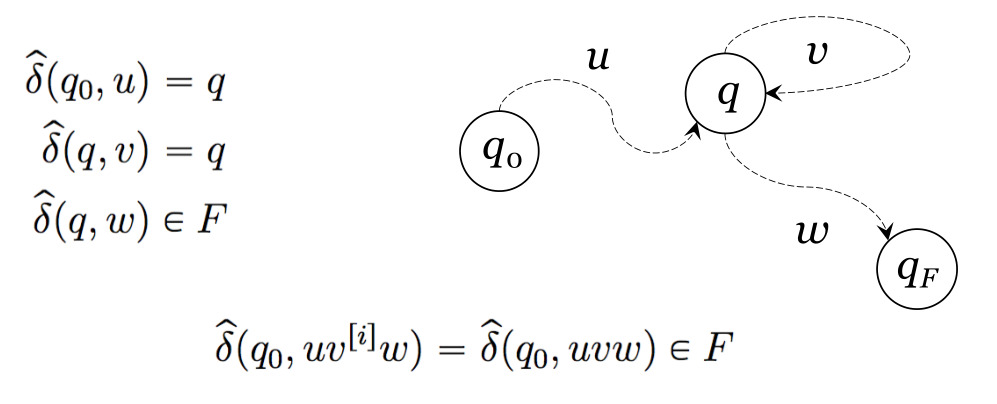
\includegraphics[ width=1.0\linewidth, height=\textheight, keepaspectratio]{./pics/pumping-lemma.jpg}
    \caption{Rappresentazione del grafo di un automa soggetto al Pumping lemma.}
    \label{fig:pumping-lemma}
\end{figure}

\begin{flushright}
$\blacksquare$
\end{flushright}

In parole povere, è come se il cammino per $v$ ``non contasse'', e si potesse
scrivere un numero arbitrario di caratteri in $v$ pur rimanendo nei confini di
un linguaggio regolare. Il \emph{Pumping lemma} può essere invece adoperato per
dimostrare la \emph{non regolarità} di un determinato linguaggio. In
particolare, si cerca ora di dimostrare la non regolarità del linguaggio $$\mathcal
L = \{a^n b^n | n \geq 0\}.$$

Per assurdo, sia $\mathcal L$ regolare, con un automa in grado di generarlo
dotato di $m$ stati. Si scelga ora $x = a^m b^m$. Poiché si suppone essere regolare, il Pumping
lemma permette di scriverlo come $x = uvw$, con $uv^{[i]}w \in \mathcal L$
avendo $i \geq 0$. Con la scelta di $i=2$ si verificano tre possibili casi. In
ciascuno di essi la stringa $x$ non può appartenere ad $\mathcal L$ e non sarà
dunque un linguaggio della forma $a^n b^n$ con $n \geq 0$.

\begin{enumerate}
    \item la stringa $v$ consiste esclusivamente di zeri. Tuttavia, così
        facendo la stringa totale dovrà per forza essere composta da un maggior
        numero di zeri che uni, infatti $uvvw$ conterrà un numero
        sovrabbondante di 0, in quanto presenti in $v$;
    \item la stringa $v$ consiste esclusivamente di uni. Il ragionamento di cui
        sopra si applica;
    \item la stringa $v$ consiste di un numero di 0 e di 1. Benché $uvvw$ possa
        disporre del medesimo numero di 0 e 1, essa non potrà mai essere della
        forma desiderata, poiché per simmetria di $vv$ avremo alcuni 1 o 0 che
        verranno prima degli altri.
\end{enumerate}


\clearpage


\section{I grafi di transizione}

\begin{definizione}[Grafo di transizione]
Un \textbf{grafo di transizione} $T$ \textbf{su} $\Sigma$ è un \emph{grafo
orientato finito} in cui ogni arco è etichettato da qualche parola $w \in
\Sigma^*$, eventualmente $w =\Lambda$ parola vuota. Esistono i vertici iniziali
e vertici finali, i primi etichettati con il segno $-$, i secondi (se esistono)
etichettati con il segno $+$. Un vertice può essere sia iniziale che finale.
\end{definizione}

In parole povere, gli archi non corrispondono ad un cambio di stato, bensì
direttamente a delle stringhe, le quali comportano gli opportuni cambiamenti di
nodo all'interno del grafo. Le parole si possono concatenare, e la parola $w$
viene accettata soltanto qualora la concatenazione delle etichette corrisponda
proprio alla parola $w$.


\begin{figure}[h]
    \centering
    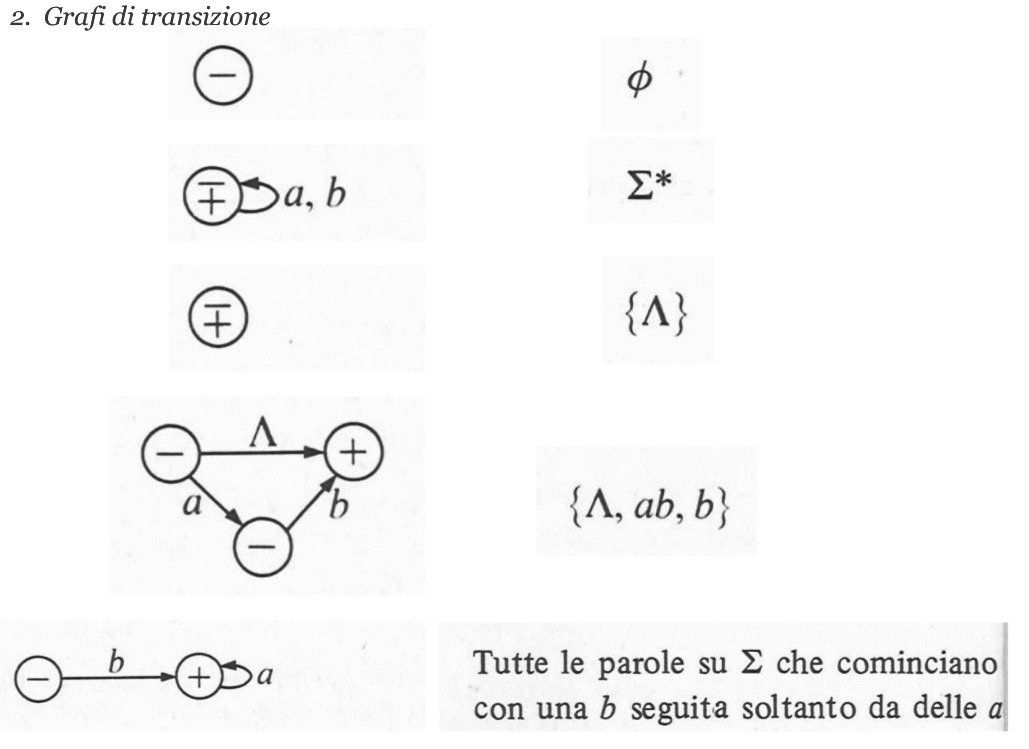
\includegraphics[ width=0.6\linewidth, height=\textheight, keepaspectratio]{./pics/automiGrafiElementari.jpg}
    \caption{Alcuni esempi base di grafi di transizione. Altri esempi sono
    forniti sulle slide.}
    \label{fig:automiGrafiElementari}
\end{figure}

\begin{figure}[ht]
    \centering
    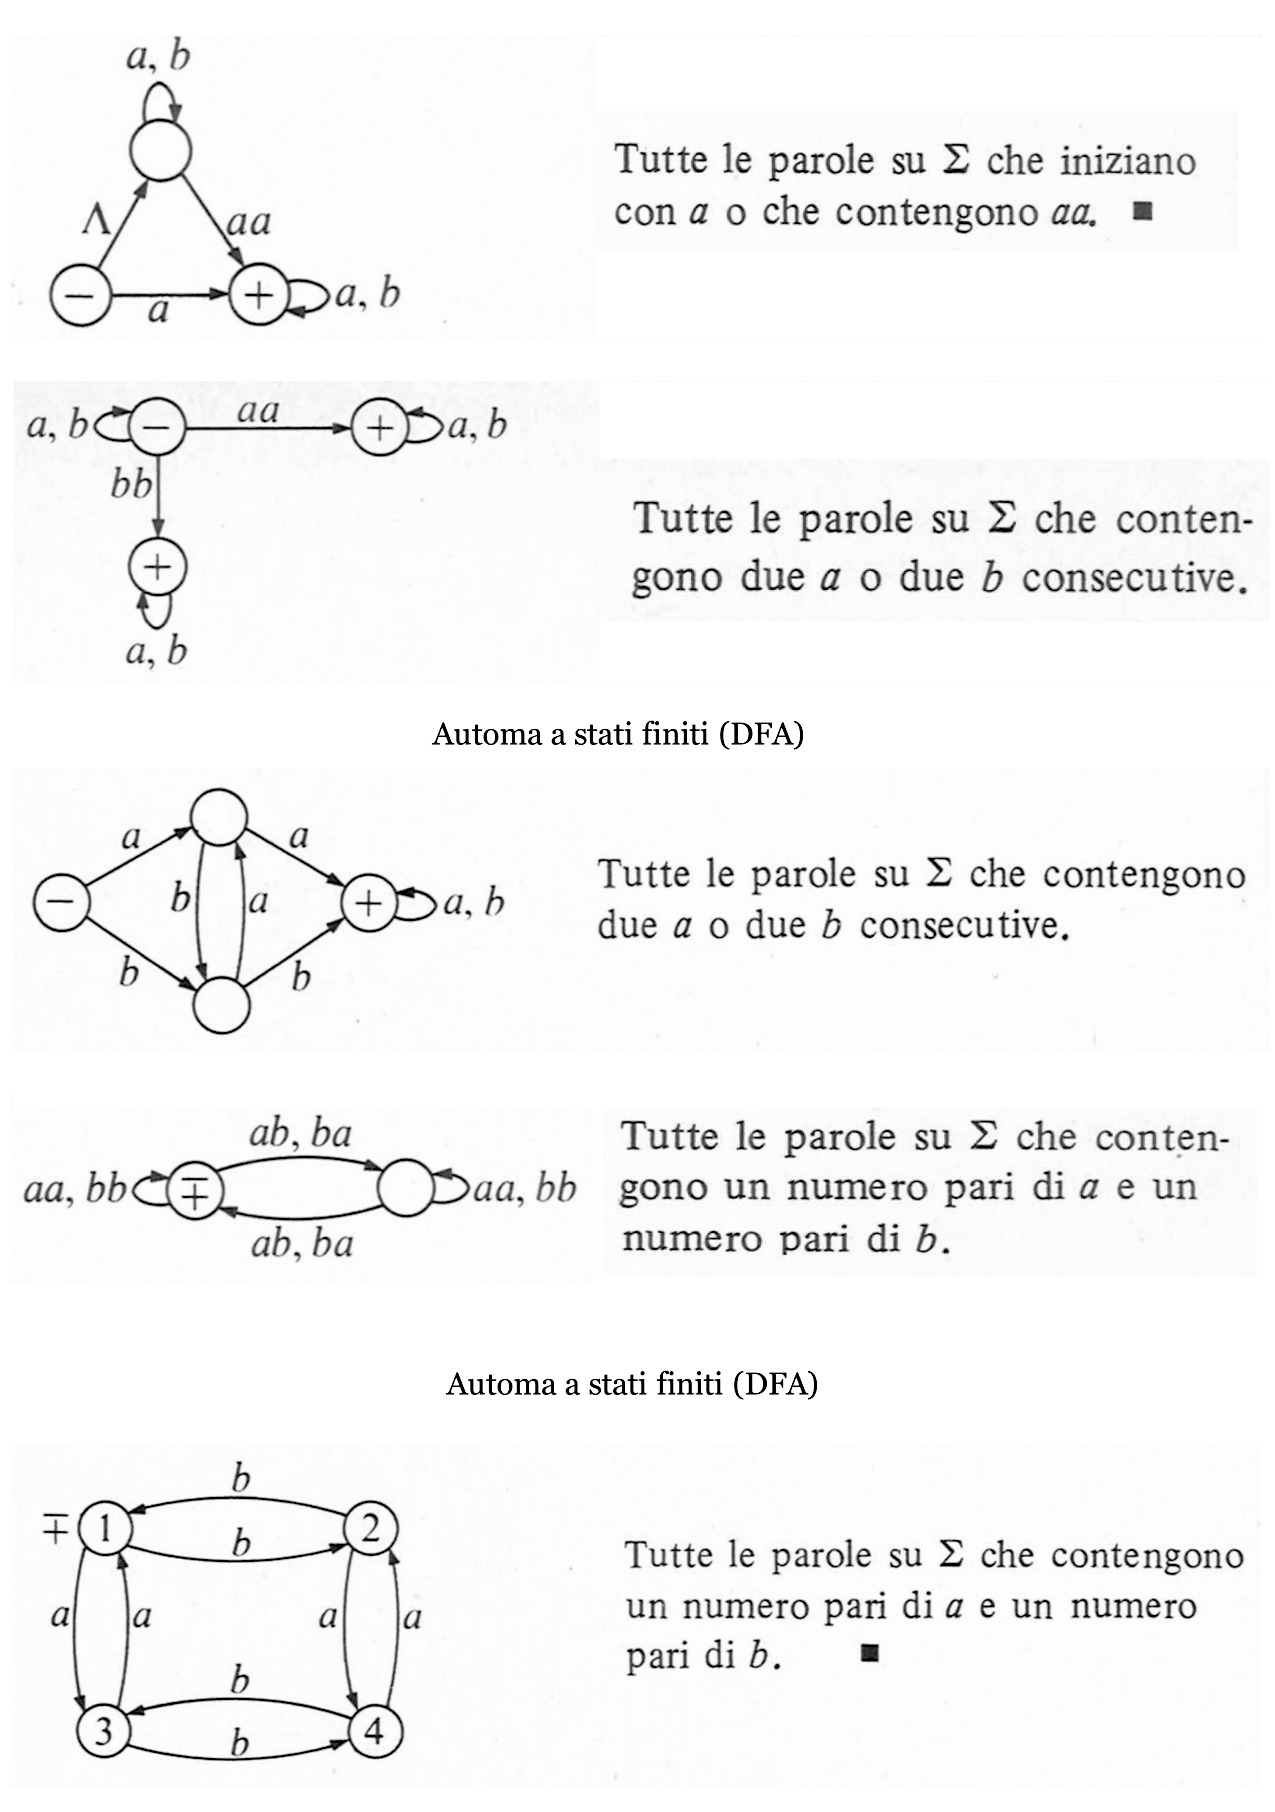
\includegraphics[ width=1.0\linewidth, height=\textheight, keepaspectratio]{./pics/grafi-transizione-esempi.jpg}
    \caption{Esempi di grafi di transizione.}
    \label{fig:grafi-transizione-esempi}
\end{figure}


Definiamo ora il \emph{$w$-cammino} per una parola $w \in \Sigma^*$ come il
cammino finito da un vertice $i$ ad un vertice $j$ nel grafo $T$ tale che la
concatenazione delle etichette sugli archi di questo cammino formi la parola
$w$, trascurando eventuali parole vuote $\Lambda$. Dunque, una parola è
\emph{accettata} da un grafo $T$ quando esiste un $w$-cammino per tale parola
dal vertice iniziale a quello finale. L'unico caso in cui la parola vuota
$\Lambda$ è accettata è quello in cui un vertice in $T$ è sia iniziale che
finale (inizia e finisce subito) o se esiste un $\Lambda$-cammino da un vertice
iniziale ad uno finale. L'insieme delle $w_a$ accettate da un grafo $T$ si
indica con la lettera $\tilde{T}$.

\clearpage

\section{Le espressioni regolari}

\begin{definizione}[Classe delle espressioni regolari]
La \textbf{classe delle espressioni regolari}\footnote{Tale definizione ricorda
la definizione degli \emph{insiemi regolari}. Infatti, come fra poco sarà illustrato, l'operazione $+$ è
riconducibile all'unione fra insiemi, l'operazione $\cdot$ è riconducibile al
prodotto fra insiemi, ed $*$ alla stellatura fra insiemi.} su $\Sigma$ è
ricorsivamente definita come segue: sia $\Sigma = \{\sigma_1, \sigma_2, \dots,
\sigma_n\}$, definiamo \emph{alfabeto accessorio} $$\Sigma_A = \{\sigma_1,
\sigma_2, \dots, \sigma_n, \Lambda, \emptyset, +, \cdot, *, (, )\}.$$ La classe
delle \textbf{espressioni regolari} su $\Sigma$ è definita come il sottoinsieme
di $\Sigma_A^*$ tale che

\begin{enumerate}
    \item $\Lambda$ e $\emptyset$ sono espressioni regolari su $\Sigma$;
    \item ogni lettera $\sigma \in \Sigma$ è un'espressione regolare su
        $\Sigma$;
    \item se $R_1$ e $R_2$ sono espressioni regolari su $\Sigma$, lo sono anche
        $R_1 + R_2$, $R_1 \cdot R_2$, ed $R_1^*$ e $R_2^*$.
\end{enumerate}
\end{definizione}

Facendo un esempio, data $\Sigma = \{a,b\}$, allora $(((a + (b\cdot a)))^*\cdot
a)$ è un'espressione regolare su $\Sigma$.

Dunque, ogni espressione regolare $R$ su $\Sigma$ descrive un \emph{insieme
$\tilde{R}$ di parole su $\Sigma$}, cioè si ha che l'insieme $\tilde{R}\subseteq
\Sigma^*$ è definito ricorsivamente come segue:
\begin{enumerate}
    \item se $R = \Lambda$, allora $\tilde R = \{\Lambda\}$, cioè è l'insieme
        costituito dalla parola vuota $\Lambda$. Se $R = \emptyset$ allora
        $\tilde R = \emptyset$, cioè è uguale all'insieme vuoto;
    \item se $R = \sigma$, allora $\tilde R = \{ \sigma \}$, cioè è l'insieme costituito dalla lettera $\sigma$;
    \item siano $R_1$ ed $R_2$ espressioni regolari su $\Sigma$ che descrivono gli insiemi di parole $\tilde R_1$ e $\tilde R_2$, rispettivamente,
\begin{itemize}
    \item se $R = (R_1 + R_2)$, allora $$\tilde R = \tilde R_1 \cup \tilde R_2
        = \{x | x \in \tilde R_1 \mbox{ oppure } x \in \tilde R_2\}$$ ovvero
        l'insieme unione;
    \item se $R = (R_1 \cdot R_2)$, allora $$\tilde R = \tilde R_1 \tilde R_2 =
        \{xy | x \in \tilde R_1 \mbox{ e } y \in \tilde R_2\}$$ ovvero
        l'insieme prodotto;
    \item se $R = (R_1)^*$, allora $$\tilde R = \tilde R_1^* =
        \{\Lambda\} \cup \{x | x \mbox{ ottenuti concatenando un numero finito
        di parole di } \tilde R_1\}$$ ovvero l'insieme chiusura;
\end{itemize}
\end{enumerate}

Facciamo ora alcuni esempi di espressioni regolari. Sia l'insieme $\Sigma = \{a,b\}$:
\begin{description}
    \item[$\bf ba^*$] Tutte le parole su $\Sigma$ che cominciano per $b$ seguite
        soltanto da delle $a$.
    \item[$\bf a^*ba^*ba^*$] Le parole su $\Sigma$ che incominciano con una sequenza di $a$,
        hanno una $b$, poi una sequenza di $a$, un'altra $b$ e terminano con
        sole $a$.
    \item[$\bf (a+b)^*$] Tutte le parole su $\Sigma$.
\end{description}

\begin{figure}[ht]
    \centering
    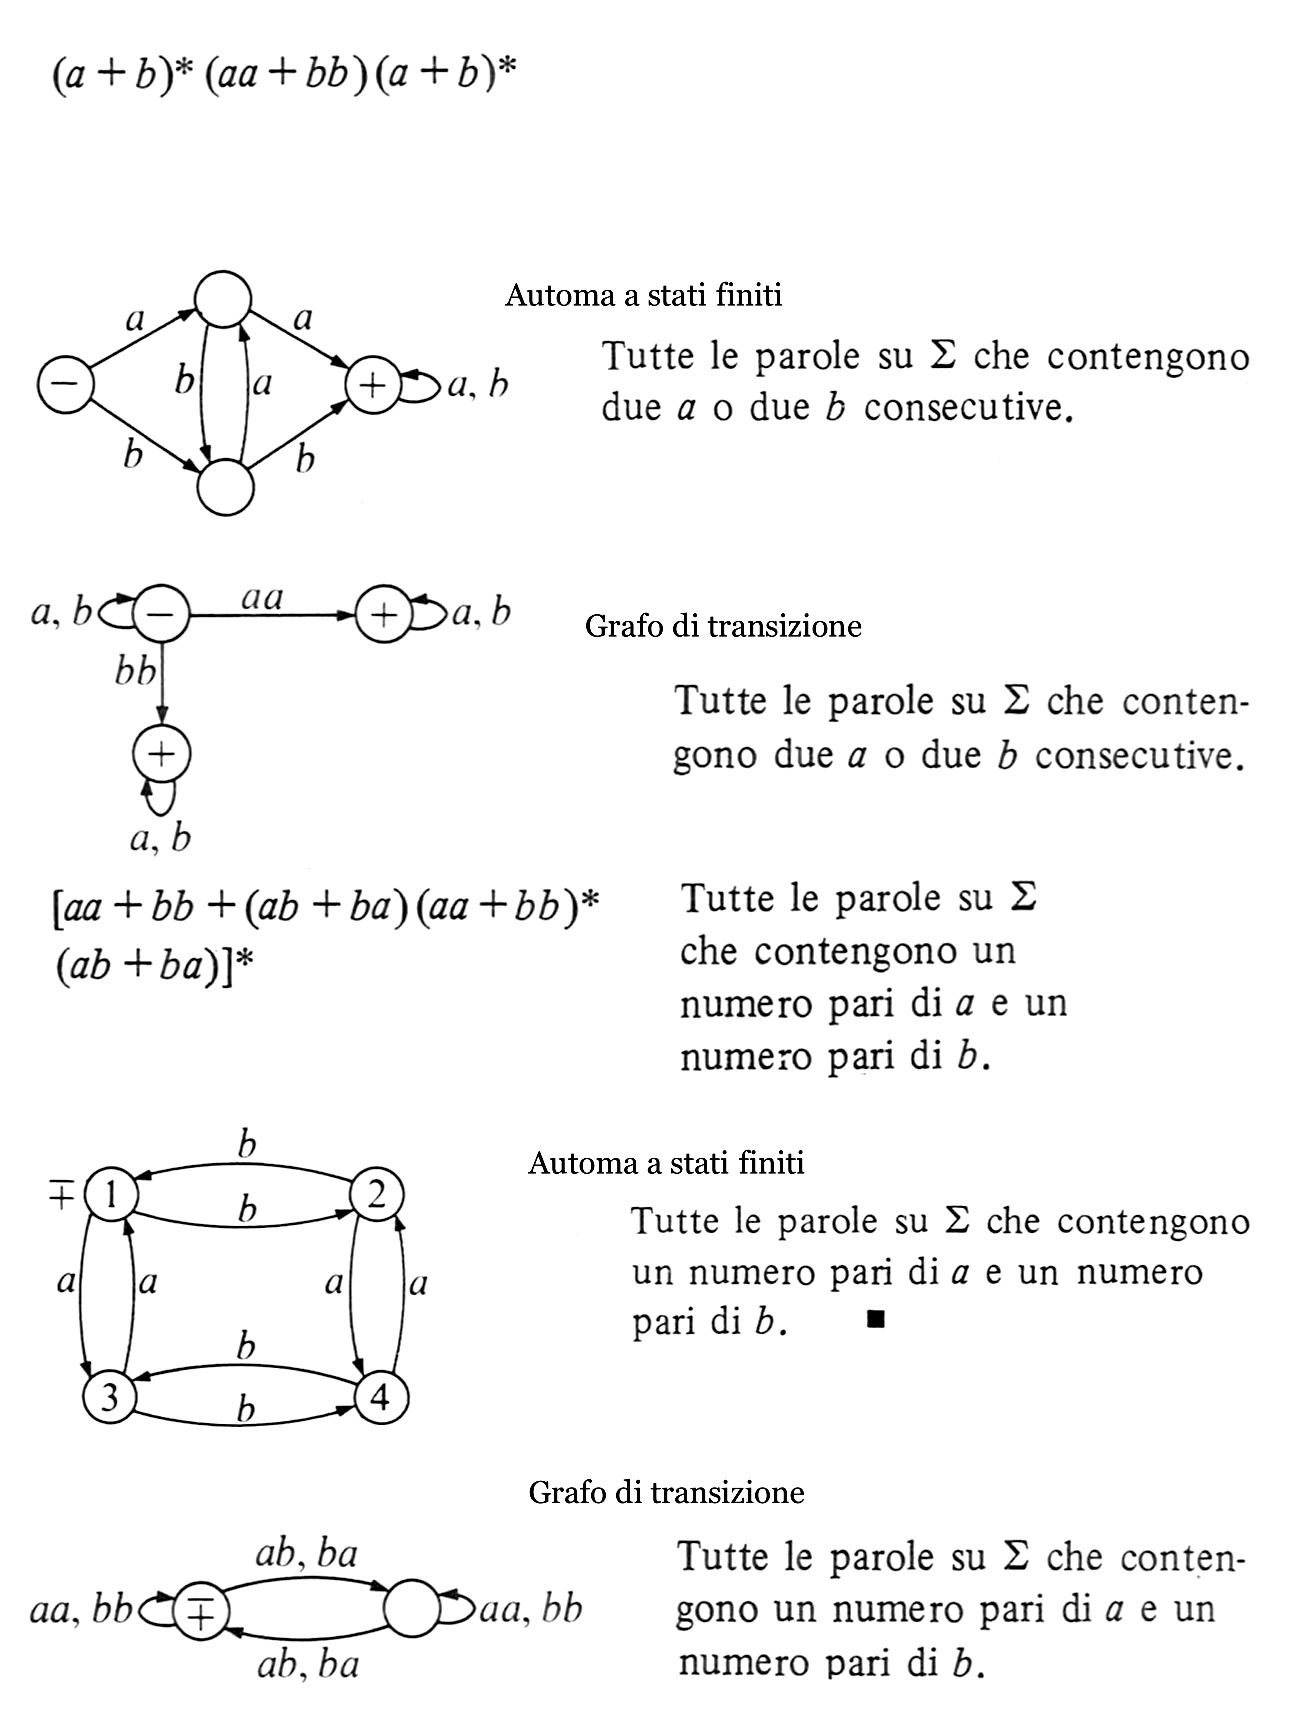
\includegraphics[ width=1.0\linewidth, height=\textheight, keepaspectratio]{./pics/espressioni-regolari-esempi.jpg}
    \caption{Esempi di espressioni regolari, con relativo automa a stati finiti
    non deterministico e grafo di transizione.}
    \label{fig:espressioni-regolari-esempi}
\end{figure}

\clearpage


Un importante risultato è che dalla definizione delle espressioni regolari,
consegue direttamente che \emph{un insieme è regolare su $\Sigma$ se e solo se
può essere espresso da una espressione regolare su $\Sigma$}. Un insieme
regolare può essere descritto da diverse espressioni regolari. Ad esempio,
tutte le parole $\Sigma = \{a, b\}$ con $a$ e $b$ che si alternano e che
cominciano e terminano con $b$ può essere descritto sia da $b(ab)^*$ che da
$(ba)^* b$.

\begin{definizione}[Equivalenza fra espressioni regolari]
Si dice che due espressioni regolari $R_1$ ed $R_2$ su $\Sigma$ sono
\emph{equivalenti} con notazione $R_1 = R_2$ se e solo se $\tilde R_1 = \tilde
R_2$.
\end{definizione}

Secondo questa definizione, le stringhe $b(ab)^*$ e $(ba)^* b$ sono
equivalenti. Infatti, l'insieme delle parole di $R_1$ combacia con l'insieme di
parole di $R_2$, poiché descrivono le medesime stringhe.

Da questa definizione sorgono varie identità interessanti. Ad esempio, 

$$  R_1 +  S_1 =  S_1 +  R_1,$$
$$  R_1 + \emptyset = \emptyset +  R_1,$$
$$  R +  R =  R,$$
$$ ( R +  S) =  T =  R + ( S +  T),$$
$$ R \Lambda  = \Lambda  R =  R,$$
$$ R \emptyset  = \emptyset  R = \emptyset,$$
$$( R  S)  T  =  R (  S  T),$$
e, in generale,
$$ R  S \neq  S  R.$$

Altre ancora sono le seguenti, 
\begin{align*}
    R(S + T) &= RS + RT;  (S + T)R = SR + TR; \\
    R^* &= R^* R^* = (R^*)^* = (\Lambda + R)^*; \emptyset^* = \Lambda^* = \Lambda; \\
    R^* &= \Lambda + R + R^2 + \cdots + R^k + R^{k+1}R^*; \mbox{ con } k \geq 0, \\
        &  \mbox{ caso particolare } R^* = \Lambda + RR^*; \\
    (R+S)^* &= (R^* + S^*)^* = (R^* S^*)^*  = (R^* S^*)R^* = R^*(SR^*)^*; \\
    R^* R &= RR^*;  R(SR)^* = (RS)^*R; \\
    (R^*S)^* &= \Lambda  + (R + S)^*S, (RS^*)^* =\Lambda + R(R + S)^*;
\end{align*}

ed infine la \emph{regola di Arden}: supponiamo $\Lambda \notin S$; allora

\begin{align*}
    R = SR + T & \mbox{ se e solo se } R = S^* T \\
    R = RS + T & \mbox{ se e solo se } R = T S^*.
\end{align*}

Si noti che in generale vale che $(R + S)^* \neq R^* + S^*$. La maggior parte
delle identità appena proposte può essere dimostrata mediante la tecnica della
\emph{dimostrazione mediante parsificazione}. Tale strategia consiste nello
riarrangiamento delle espressioni di modo da ottenere la tesi, in un
procedimento che è detto ``riparsificazione'' dell'espressione.

Ad esempio, supponiamo di voler dimostrare la seguente identità.

\begin{identita}[$R(SR)^* = (RS)^* R$]
    È vero che $R(SR)^* = (RS)^* R$.
\end{identita}

\textsc{Dimostrazione } --- Si consideri qualunque parola $w \in R(SR)^*$, cioè
una parola composta nella seguente maniera:
$$r_0(s_1r_1)(s_2r_2)(s_3r_3)\cdots(s_nr_n),$$ considerando un qualche $n \geq
0$, con $n \in \mathbb{N}$, e dove ogni $r_i \in R$ e ogni $s_i \in S$. Ora,
\emph{riparsificando} la stringa ottenuta tramite associatività si ottiene
$$(r_0s_1)(r_1s_2)(r_2s_3)(r_3s_4)\cdots(r_{n-1}s_n)r_n.$$ Pertanto, la stringa
$w$ ottenuta apparterrà a $w \in (RS)^*R$, e siccome $w$ è stata scelta in modo
del tutto arbitrario ciò implica che $R(SR)^* \subseteq (RS)^* R$. In modo
analogo si dimostra il viceversa $R(SR)^* \supseteq (RS)^* R$, perciò si
ottiene l'equivalenza fra le due espressioni regolari come da identità.

\begin{flushright}
$\blacksquare$
\end{flushright}

Alternativamente, si possono adoperare identità già note per dimostrarne altre
nuove. Ad esempio, $R = S^* T$ implica $R = SR + T$ viene dimostrata a partire
da altre identità (per approfondimenti, slide 63).

In definitiva, con tutta la trattazione teorica di cui sopra sono stati
prodotti tre modelli del tutto equivalenti: il modello dell'\emph{automa a
stati finiti}, il modello del \emph{grafo di transizione} ed infine quello
delle \emph{espressioni regolari}. I tre modelli sono intercambiabili, è
possibile descrivere l'uno mediante l'altro, e hanno tutti la capacità
computazione di ``Livello 0'', quella in grado di produrre gli \emph{insiemi
regolari}. Rappresentano dunque il livello più basso della capacità
computazionale.

L'anello di congiunzione fra questi tre modelli è rappresentato da un
importante teorema, detto \emph{Teorema di Kleene}, che ci accingiamo a
dimostrare. Prima di fare ciò, però, è necessario illustrare la nozione di
\emph{grafo generalizzato}.

\begin{definizione}[Grafo di transizione generalizzato]
    Il grafo di transizione $T$ è un \emph{grafo di transizione generalizzato} se i suoi archi possono essere
    etichettati anche da espressioni regolari invece che soltanto da parole.
\end{definizione}

\begin{thm}[Kleene]
    Sia $T$ un \emph{grafo di transizione su $\Sigma$}. Allora
\begin{enumerate}
    \item per ogni grafo di transizione $T$ su $\Sigma$ esiste un'espressione regolare $R$ su $T$ tale che $\tilde R = \tilde T$; 
    \item per ogni espressione regolare $R$ su $\Sigma$ esiste un automa finito $A$ su $\Sigma$ tale che $\tilde A = \tilde R$.
\end{enumerate}
\end{thm}

\textsc{Dimostrazione } --- Per dimostrare il primo punto si descrive un
algoritmo che genera un'espressione regolare $R$ a partire da un grafo di
transizione $T$ tale che $\tilde R = \tilde T$. 

Si proceda aggiungendo al grafo $T$ un vertice $x$ e degli archi $\Lambda$ che
collegano tale vertice con tutti i vertici iniziali di $T$. Alla stessa
maniera, si aggiunga un vertice $y$ collocato ``alla fine'' del grafo, cioè
aggiungendo degli archi $\Lambda$ che conducono dai vertici finali di $T$ ad
$y$. Il nuovo grafo modificato dovrà avere un unico vertice iniziale, $x$, ed
un unico vertice finale, $y$. Un esempio di tale configurazione è mostrato in
Figura~\ref{fig:kleene1}. Il nuovo grafo di transizione dovrà essere un
\emph{grafo di transizione generalizzato} e lo indicheremo con $T'$.
Inizialmente, i suoi archi non comprenderanno alcuna espressione regolare, ma
soltanto parole.

\begin{figure}[ht]
    \centering
    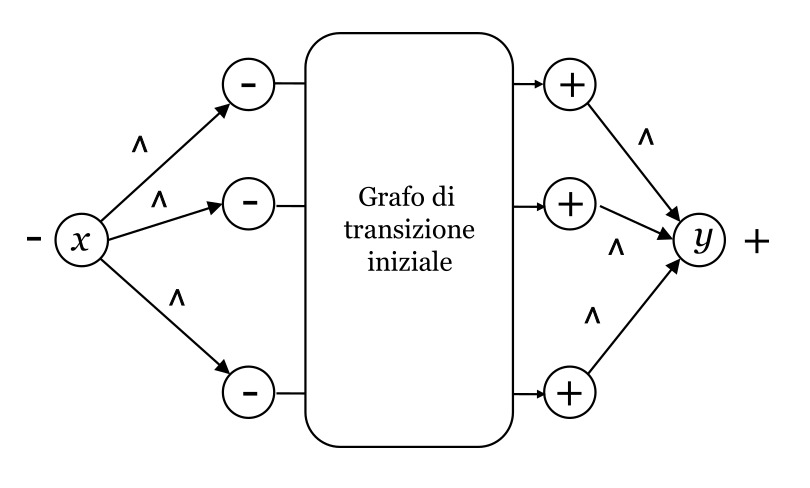
\includegraphics[ width=0.7\linewidth, height=\textheight, keepaspectratio]{./pics/kleene1.jpg}
    \caption{Nuovo grafo che vede aggiunti un vertice iniziale $x$ ed un
    vertice finale $y$, collegati al grafo precedente tramite archi $\Lambda$,
rispettivamente, ai precedenti vertici iniziali e finali.}
    \label{fig:kleene1}
\end{figure}

La parte successiva della dimostrazione consiste nell'eliminare tutti i vertici
del nuovo grafo $T'$ fintanto che non saranno presenti esclusivamente i nuovi
vertici $x$ ed $y$. Il nuovo arco ottenuto conterrà l'espressione regolare $R$
tale che $\tilde T = \tilde R$, e il primo punto sarà dimostrato. Durante il
processo di eliminazione, etichette ed archi vengono modificati. Gli archi
possono essere etichettati da espressioni regolari ($T'$ è un grafo
generalizzato). Il grafo generalizzato $T'$ accetta ancora lo stesso insieme di
parole del grafo $T$, e ad ogni rimozione o cambiamento effettuato in maniera
opportuna il nuovo grafo prodotto accetterà ancora il medesimo insieme di
parole. Il processo termina quando otteniamo un grafo come quello in
Figura~\ref{fig:kleene2}, ovverosia con i due soli vertici $x$ ed $y$;
l'espressione regolare $R$ risultante sarà $\alpha_1 + \alpha_2 + \cdots +
\alpha_n$.

\begin{figure}[ht]
    \centering
    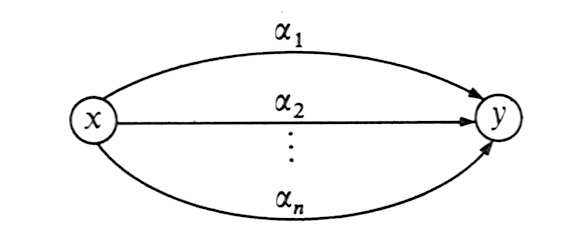
\includegraphics[ width=0.7\linewidth, height=\textheight, keepaspectratio]{./pics/kleene2.jpg}
    \caption{Grafo di transizione generalizzato risultante a seguito del
    procedimento algoritmico che ne ha portato la formazione. Esistono
unicamente due vertici $x$ ed $y$, ed ogni arco $i$-esimo è etichettato con
l'espressione regolare $\alpha_i$.}
    \label{fig:kleene2}
\end{figure}


\begin{figure}[ht]
    \centering
    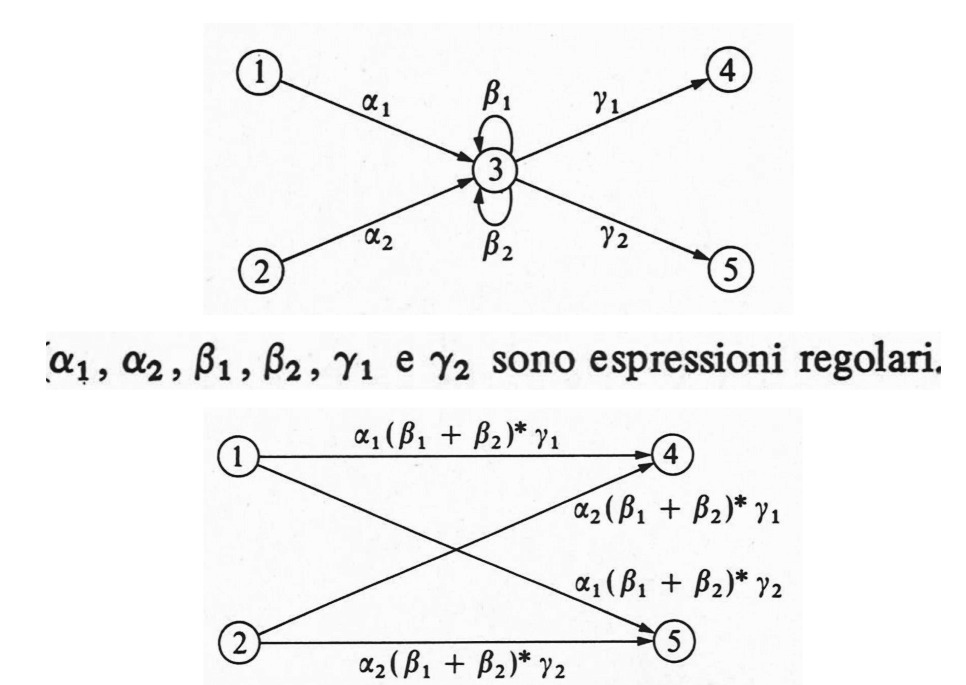
\includegraphics[ width=0.7\linewidth, height=\textheight, keepaspectratio]{./pics/kleene3.jpg}
    \caption{Procedimento di rimozione del nodo 3.}
    \label{fig:kleene3}
\end{figure}


\begin{figure}[ht]
    \centering
    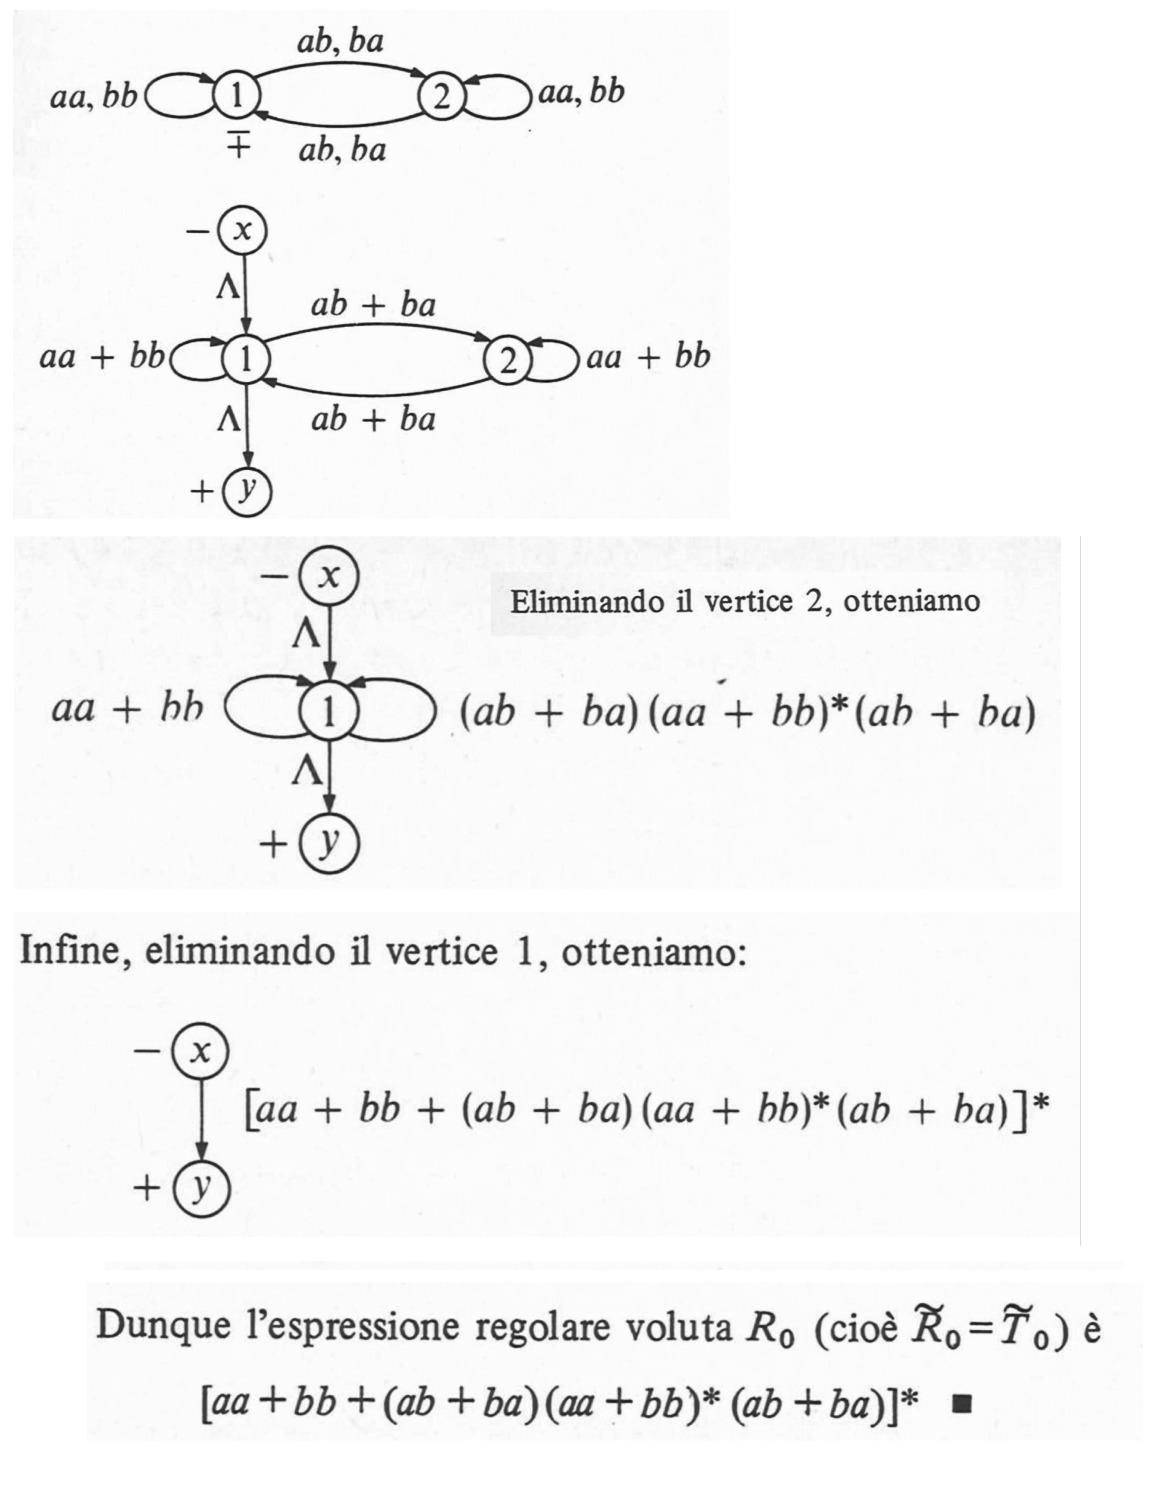
\includegraphics[ width=0.7\linewidth, height=\textheight, keepaspectratio]{./pics/kleene4.jpg}
    \caption{Esempio di procedimento completo di trasformazione di un grafo di transizione, dall'alto verso il basso.}
    \label{fig:kleene4}
\end{figure}

\clearpage

Per il punto 2, descriviamo un procedimento algoritmico noto come \emph{metodo
del sottoinsieme} per costruire, a partire da una data espressione regolare
$R$, un automa finito $A$ tale che $\tilde A = \tilde R$. Si procede a tal
proposito in tre passi:
\begin{enumerate}
    \item si costruisce un grafo di transizione $T$ tale che $\tilde T = \tilde
        R$. Si comincia con un grafo di transizione generalizzato della forma
        mostrata in Figura~\ref{fig:kleene5}. Si divide in più parti
        l'espressione regolare $R$ aggiungendo opportunamente nuovi vertici ed
        archi, finché tutti loro siano etichettati da lettere oppure da
        $\Lambda$. Si adoperano le regole mostrate in Figura~\ref{fig:kleene6};
    \item sia $T$ il grafo di transizione generato seguendo i due passi
        precedenti. Si costruirà la \emph{tabella di transizione} di $T$.
        Supponiamo, per semplicità, che $\Sigma = \{a,b\}$. Sia $M$ un
        qualunque sottoinsieme di vertici del grafo di transizione $T$; per
        qualunque parola $w \in \Sigma^*$ definiamo $M_w$ il sottoinsieme di
        tutti i vertici di $T$ che possono essere raggiunti con un $w$-cammino
        da qualche vertice di $M$. Ad esempio, $M_{ab}$ è l'insieme dei vertici
        di $T$ raggiungibili con un $ab$-cammino a partire da un vertice di
        $M$. Similmente, esso è anche l'insieme dei vertici di $T$
        raggiungibili con un $b$-cammino stavolta a partire da un vertice di
        $M_a$. Esso è schematizzato in Figura~\ref{fig:kleene7};
    \item l'ultimo passo consiste nel utilizzare la tabella di transizione per
        costruire l'automa finito $A$ desiderato. In particolare, ad ogni
        sottoinsieme $M$ della colonna 1 della tabella corrisponde un vertice
        $\bar M$ per l'automa $A$. Da ogni vertice $\bar M$ di $A$ si diparte
        un arco $a$ che conduce al vertice $M_a$, e un arco $b$ che conduce dal
        vertice $\bar M_b$. Il vertice $\{\bar x\}_\Lambda$, corrispondente al
        sottoinsieme nell'angolo sinistro superiore della tabella) è il solo
        vertice iniziale dell'automa $A$. Un vertice $\bar M$ di $A$ è finale
        se e solo se $M$ contiene un vertice finale di $T$.
\end{enumerate}

\begin{figure}[ht]
    \centering
    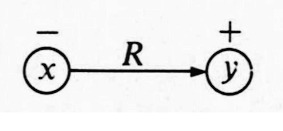
\includegraphics[ width=0.5\linewidth, height=\textheight, keepaspectratio]{./pics/kleene5.jpg}
    \caption{Grafo di transizione generalizzato di partenza per il primo passo.}
    \label{fig:kleene5}
\end{figure}

\begin{figure}[ht]
    \centering
    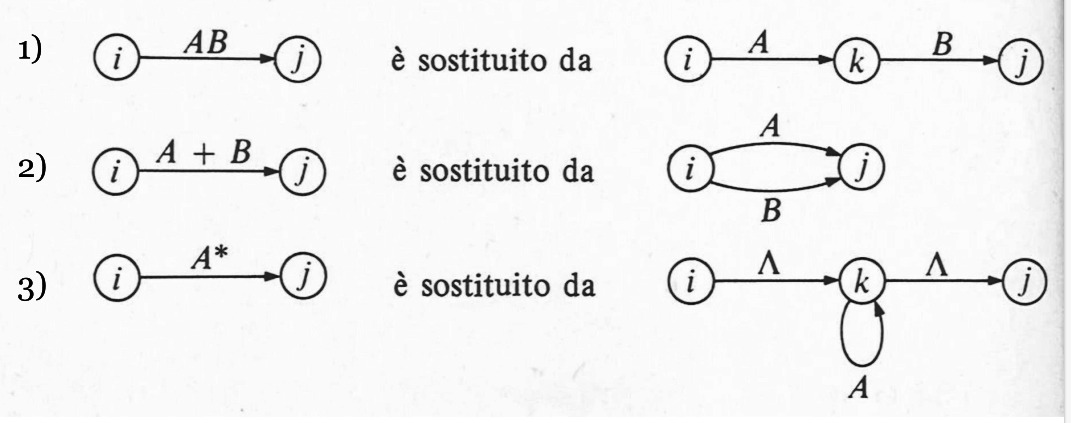
\includegraphics[ width=1.0\linewidth, height=\textheight, keepaspectratio]{./pics/kleene6.jpg}
    \caption{Regole di sostituzione per il passo due.}
    \label{fig:kleene6}
\end{figure}

\begin{figure}[ht]
    \centering
    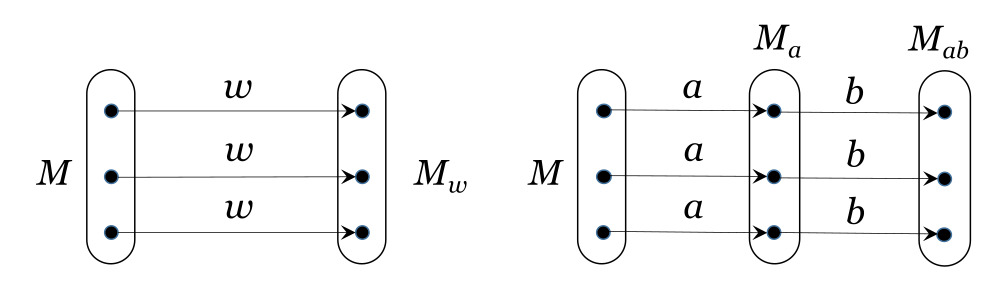
\includegraphics[ width=1.0\linewidth, height=\textheight, keepaspectratio]{./pics/kleene7.jpg}
    \caption{Illustrazione del $w$-cammino e del $ab$-cammino lungo i sottoinsiemi di vertici $M$, $M_a$ ed $M_{ab}$.}
    \label{fig:kleene7}
\end{figure}



Dunque, il teorema è dimostrato.

\begin{flushright}
$\blacksquare$
\end{flushright}


\clearpage

Dal momento che ogni automa finito è un grafo di transizione, dal teorema
seguono immediatamente i seguenti fatti:
\begin{itemize}
    \item un insieme è regolare su $\Sigma$ se e solo se è accettato da qualche automa finito su $\Sigma$;
    \item un insieme è regolare su $\Sigma$ se e solo se è accettato da qualche grafo di transizione su $\Sigma$.
\end{itemize}

Un ultimo esempio è quello fornito dalla Figura~\ref{fig:kleene8}.

\begin{figure}[ht]
    \centering
    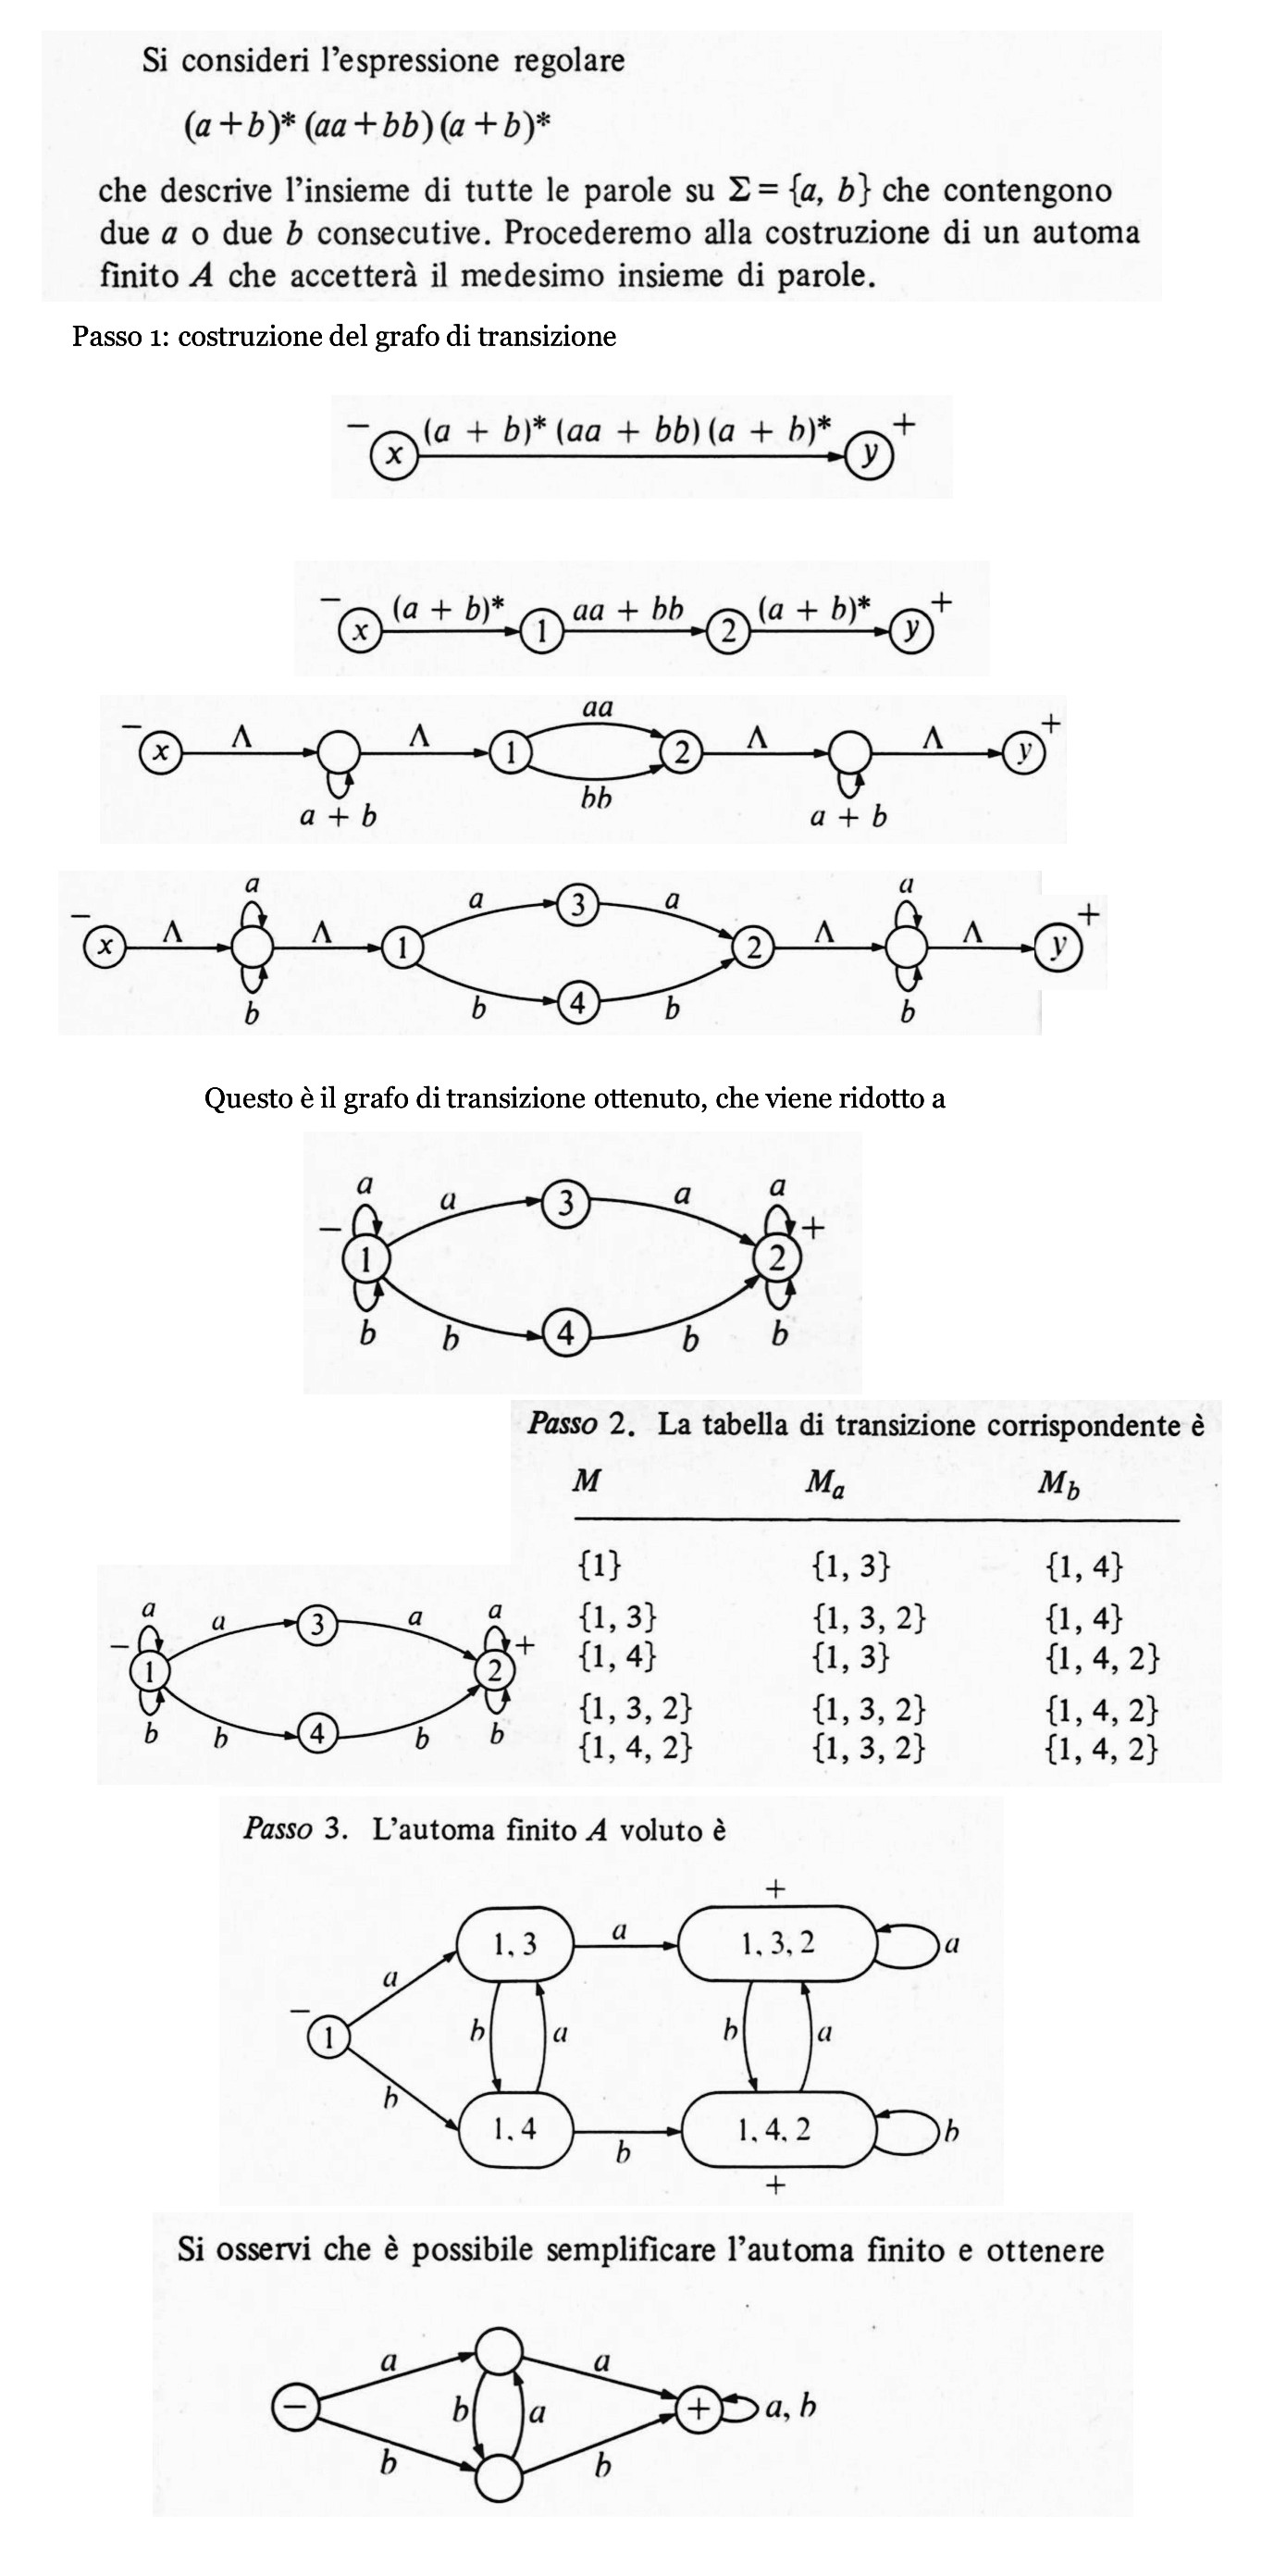
\includegraphics[ width=1.0\linewidth, height=\textheight, keepaspectratio]{./pics/kleene8.jpg}
    \label{fig:kleene8}
\end{figure}

\clearpage

\chapter{Le grammatiche}

Una \textbf{grammatica} è, intuitivamente, un insieme di regole che permettono
di generare un \emph{linguaggio}. Fra le possibili grammatiche, una categoria
in particolare riveste un ruolo importante, la categoria delle
\emph{grammatiche libere dal contesto}, dette anche \emph{Context-Free
Grammars} e abbreviate con CF. Tramite le grammatiche libere dal contesto viene
descritta la sintassi dei linguaggi di programmazione. In parole povere, le
grammatiche sono un modo ulteriore per generare insiemi di stringhe, appunto
dei linguaggi.

Una stringa appartiene ad un linguaggio quando essa è stata generata mediante
le \emph{production rules} a partire da una stringa già appartenente al
linguaggio. Si parte innanzitutto da una stringa. Adoperando le production
rules si ottiene una nuova stringa modificata: quest'ultima appartiene ancora
al linguaggio.

\subsubsection{Grammatiche di tipo 0}

Le prime tipologie di grammatiche sono dette \emph{grammatiche di tipo 0} o
\emph{grammatiche a struttura di frase}. Queste grammatiche sono definite a
partire da una quadrupla. 

\begin{definizione}[Grammatica di tipo 0 o a struttura di frase] Una \emph{grammatica di tipo 0} o \emph{a struttura di frase} è una quadrupla $$G = \langle V, \Sigma, P, S\rangle$$ dove 
\begin{itemize}
    \item $V$ è un insieme finito di variabili, dette anche \emph{simboli non terminali}; 
    \item $\Sigma$ è un insieme finito di \emph{simboli terminali} tale che $V \cap \Sigma =
\emptyset$; 
    \item $P$ è un insieme finito di \emph{produzioni} (le production rules),
        con ogni produzione della forma $$\alpha \rightarrow \beta,$$ (al posto
        di $\alpha$ si sostituisce $\beta$; sono dette anche \emph{regole di
        riscrittura}) e inoltre $\alpha \in (V \cup \Sigma)^+ = (V \cup
        \Sigma)^* - \{\Lambda\}$ e $\beta \in (V \cup \Sigma)^*$;
    \item $S \in V$ è il \emph{simbolo inziale}.
\end{itemize}
\end{definizione}

Le variabili non terminali saranno indicate dalla lettera maiuscola, mentre
tutti i simboli terminali saranno denotati con la lettera minuscola.

Data la definizione di grammatica di tipo 0, ci accingiamo a illustrare le
possibili maniere in cui una parola di una certa grammatica possa essere
generata da tale grammatica. L'insieme di tali parole generabili si dirà
linguaggio.

Una parola $w \in \Sigma^*$ si dice \emph{generata} da $G$ se esiste una
sequenza finita di parole su $V \cup \Sigma$ (produzione) tale che $$S = w_0
\Rightarrow w_1 \Rightarrow w_2 \Rightarrow \cdots \Rightarrow w_n, \mbox{ con
} n \geq 1$$ tali che $w_0$ sia la variabile d'inizio $S$, e $w_n = w$ e la
parola successiva $w_{i+1}$ sia ottenuta da $w_i, 0 \leq i < n$, sostituendo
qualche occorrenza di una sottostringa $\alpha$ che sia dal lato sinistro di
qualche produzione di $P$ in $w_i$ con il $\beta$ corrispondente che sia dal
lato destro della produzione stessa. L'insieme delle parole generate da $G$ si
dice \emph{linguaggio generato da $G$}.

Ad esempio, sia $\Sigma = \{a, b\}$, e si consideri la grammatica $G_1$ con $V
= \{S\}$ e $P = \{S \rightarrow aSb, S \rightarrow ab\}.$ Applicando la prima
produzione $n-1$ volte e facendo seguire un'applicazione della seconda
produzione alla fine, si ottiene la nuova parola

$$S \Rightarrow aSb \Rightarrow a^2Sb^2 \Rightarrow \cdots \Rightarrow
a^{n-1}Sb^{n-1} \Rightarrow a^{n}b^{n}.$$ È chiaro che queste sono le sole
parole generate dalla grammatica, cosìcché il linguaggio generato dalla
grammatica $G_1$ sarà proprio l'insieme di parole $$\mathcal L = \{a^n b^n | n\geq 1\}.$$

Un insieme di parole su $\Sigma$ è un \emph{linguaggio di tipo 0} se può essere
generato da qualche grammatica di tipo 0 su tale $\Sigma$. Il seguente teorema
consolida tale affermazione.

\begin{thm}[Chomsky]
    Un insieme di parole su $\Sigma$ è \emph{ricorsivamente numerabile} se e
    solo se è un linguaggio di tipo 0.
\end{thm}

A tal proposito, ricordiamo che un insieme è detto ricorsivamente numerabile se
$C_A$ è parzialmente computabile, cioè se il predicato $x \in A$ è
semidecidibile. Dal teorema segue il seguente predicato:

\begin{center}
\begin{quote}
    \emph{Esiste una macchina di Turing che accetta ogni parola in $S$ e rifiuta o
    cicla per ogni parola in $\Sigma^* - S$.}
\end{quote}
\end{center}

Restrizioni sulla natura delle produzioni di una grammatica di tipo 0 possono
essere fatte, dando così origine ad altri tre tipi di grammatiche costruite
sopra la numero zero. Una grammatica può essere, pertanto,
\begin{description}
    \item[Tipo 1 (sensibile al contesto)] se per ogni produzione $\alpha
        \rightarrow \beta$ in $P$ si ha che $|\alpha| \leq |\beta|$. Essa ha
        vincoli sulla lunghezza della stringa;
    \item[Tipo 2 (libera dal contesto, Context-Free)] se per ogni produzione
        $\alpha \rightarrow \beta$ in $P$ si ha che $\alpha \in V$ e che $\beta
        \in (V \cup \Sigma)^+$. Essa equivale ad automi con 1 memoria
        push--down;
    \item[Tipo 3 (regolare)] se ogni produzione in $P$ è della forma $$A
        \rightarrow \sigma B$$ oppure $$A \rightarrow \sigma,$$ cioè sono
        grammatiche in cui i simboli terminali stanno solo a destra. Le
        grammatiche di tipo 3 esprimono gli insiemi ed i linguaggi regolari,
        pertanto sono equivalenti ad automi a stati finiti.
\end{description}

È opportuno soffermarsi ora sulle grammatiche di Tipo 2, quelle libere dal
contesto. Storicamente, esse furono adoperate per studiare la struttura delle
lingue naturali, e rappresentano facilmente delle stringhe con struttura
ottenibile mediante ricorsione. Fra le applicazioni rientrano i \emph{parser}
per compilatori ed interpreti, i quali fanno ampio uso delle grammatiche di
tipo 2.

La differenza principale fra una grammatica di tipo 2 ed una di tipo 0 risiede
nella definizione dell'$\alpha$ nella produzione $\alpha \rightarrow \beta$:
nel caso delle grammatiche di tipo 0, $\alpha \in (V \cup \Sigma)^+$, mentre
nel caso di quelle di tipo 2 si ha soltanto $\alpha \in V$. In altre parole,
\emph{a sinistra ci sono soltanto variabili}. Un'altra piccola differenza sta
nella definizione della variabile $\beta$: non più $\beta \in (V \cup
\Sigma)^*$, bensì $\beta \in (V \cup \Sigma)^+$. Un linguaggio generato da una
grammatica libera dal contesto prende il nome di \emph{Context-Free Language
(CFL)}.

Alcuni esempi di Context-Free language sono dati dalla
Figura~\ref{fig:context-free}.

\begin{figure}[ht]
    \centering
    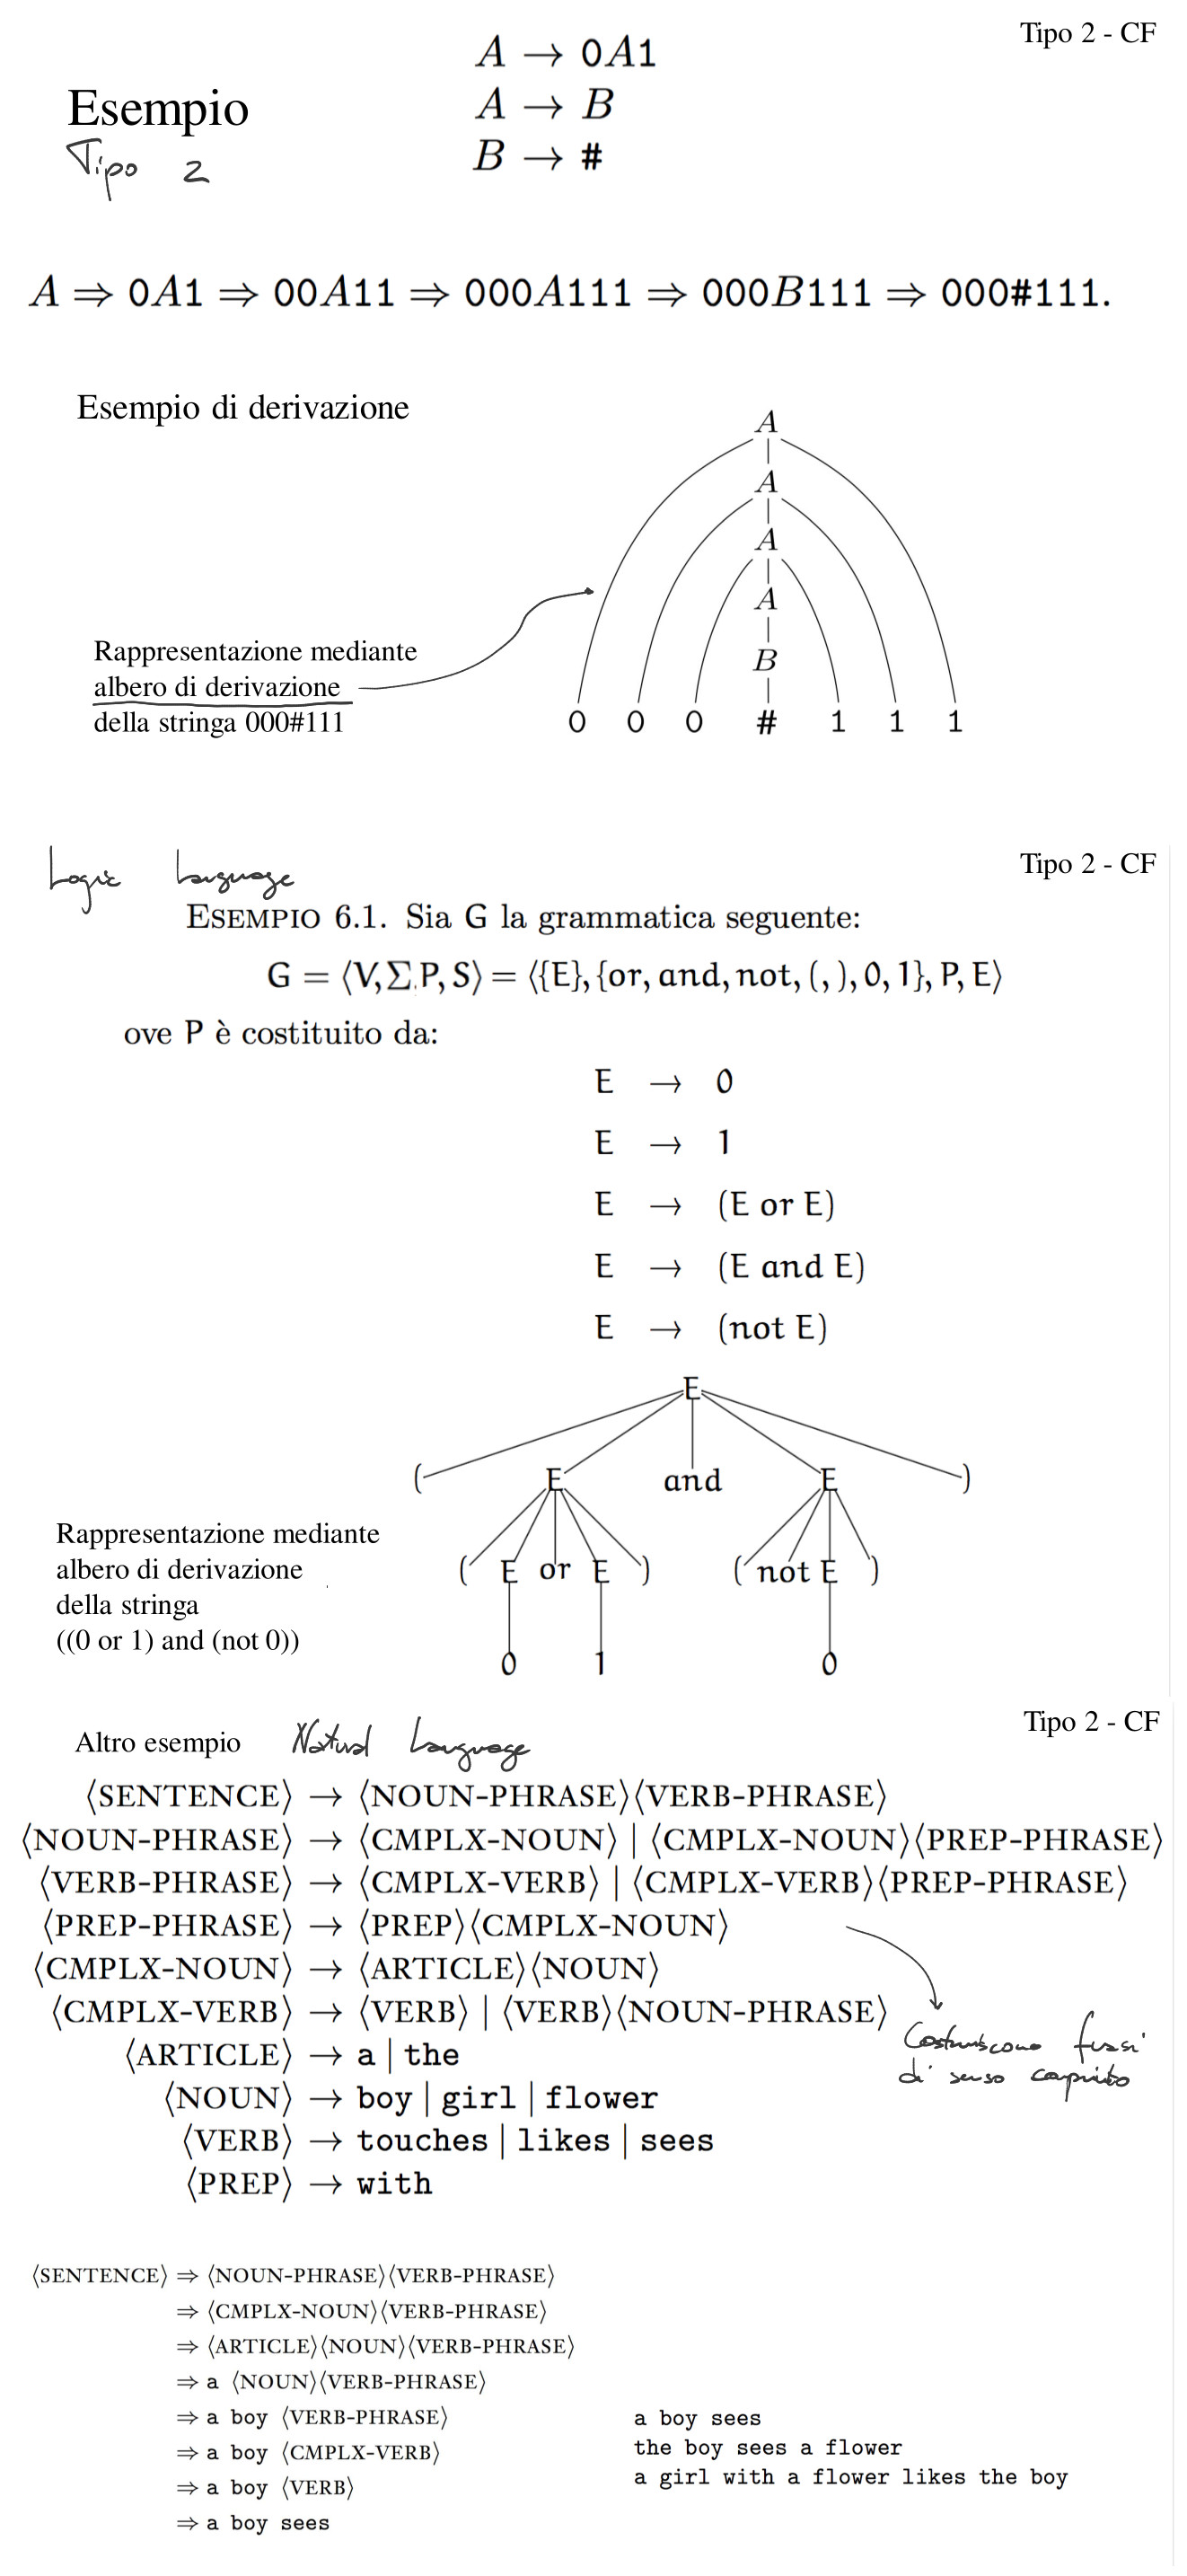
\includegraphics[ width=0.7\linewidth, height=\textheight, keepaspectratio]{./pics/context-free.jpg}
    \caption{Esempi di derivazioni di frasi e di stringhe mediante l'uso di
    grammatiche di tipo 2.}
    \label{fig:context-free}
\end{figure}

Una grammatica libera dal contesto viene solitamente specificata in una forma
più consona alla trattazione. Sia una grammatica di tipo 2 con $\alpha \in V$ e
$\beta \in (V \cup \Sigma)^+$; si dice che tale grammatica è in \emph{forma
normale di Chomsky} se ogni produzione è della forma

\begin{align}
    A & \rightarrow BC & A, B, C \in V \\
    A & \rightarrow \sigma & \sigma \mbox{ simbolo terminale }
\end{align}

con $B$ e $C$ che non possono essere variabili iniziali, e la produzione $S
\rightarrow \Lambda$ con $S$ variabile iniziale viene accettata. Si può
dimostrare che ogni grammatica libera dal contesto può essere resa in forma
normale.

Le grammatiche libere dal contesto sono equivalenti a degli automi a pila.
Infatti, il teorema seguente (senza dimostrazione) ne evidenzia l'affinità.

\begin{thm}
    Un linguaggio è \emph{libero dal contesto} se e solo se può essere generato
    da una macchina non deterministica con 1 memoria push--down, detto automa a
    pila.
\end{thm}

Il seguente teorema non è certamente l'unico relativo alle equivalenze fra
livelli di computazione e linguaggi. Difatti è possibile tracciare delle
equivalenze dirette fra tipi di macchine e linguaggi, come vedremo ora.

I \emph{linguaggi di tipo 0} sono equivalenti agli insiemi ricorsivamente
enumerabili, che sono anche gli insiemi accettati da qualche macchina finita
con due memorie pushdown. Questi linguaggi, detti a struttura di frase, sono
equivalenti alla macchina di Turing. Le loro regole di produzione sono
completamente libere: $\alpha$ e $\beta$ possono avere qualsiasi natura, fatta
eccezione per $\beta$, che non può essere $\Lambda$.

Immediatamente sotto alla gerarchia incontriamo gli insiemi ricorsivi. A
seguire, si incontrano i \emph{linguaggi di tipo 1} e successivamente i
\emph{linguaggi di tipo 2}. Questi ultimi sono equivalenti a tutti gli insiemi
accettati da qualche macchina finita non deterministica con una singola memoria
pushdown. I linguaggi di tipo 2 sono legati a grammatiche libere dal contesto,
e sono dunque equivalenti agli automi a pila.

Infine, i \emph{linguaggi di tipo 3} fanno da fanalino di coda, con
l'equivalenza fra insiemi regolari, insiemi che sono accettati da qualche
macchina finita senza memorie pushdown. Perciò, un linguaggio regolare sarà
equivalente ad un automa a stati finiti senza memoria.



\end{document}
% --------------------------------------------------------------------------------
%                        _____ _          ___         _
%                       |_   _| |_  ___  | __|_ _  __| |
%                         | | | ' \/ -_) | _|| ' \/ _` |
%                         |_| |_||_\___| |___|_||_\__,_|
%
% --------------------------------------------------------------------------------
